\chapter{Concepts}
\label{chap:Concepts}

Boot stages
\begin{verbatim}
1. BIOS code or UEFI code
2. MBR code
3. VBR code
4. (second-stage bootloader): NTLDR
combined(2.3.4) = GRUB or LILO
5. Kernel stage: Linux kernel or Windows kernel
\end{verbatim}

\section{Evolution of operating system}

First is the evolution of how a machine is booted, switching from using BIOS to
UEFI (Sect.\ref{sec:BIOS_UEFI}). Once the O/S kernel is loaded, where is
multiple stages, depending on the O/S.

Second is the evolution of O/S from single task to time-sharing CPU scheduling.
CPU cycles were no longer wasted when one process blocked on I/O.

Third is the evolution of physical memory addressing to virtual memory space.
This is managed by the O/S. (Physical) memory could be more efficiently
allocated to processes and each process could operate under the illusion that it
had an isolated address space. 

Fourth is the evolution of {\bf hypervisor} (Sect.\ref{sec:hypervisor}). The
hypervisor has a scheduler, as does the kernel.  The hypervisor has to manage
memory, as does the kernel, and so on; everything that a hypervisor does is also
part of the kernel's duties. So the guest O/S kernel has to do everything like
the host O/S kernel.

Fifth is the evolution from hypervisor to {\bf container}
(Sect.\ref{sec:containers_Linux}). This allows the host O/S kernel to support
all of the resource-isolation use cases, without the overhead and complexity of
running multiple kernel instances.
 
\url{http://lwn.net/Articles/524952/}

\section{Booting the system}
\label{sec:BIOS_UEFI}

This session describes the order of execution of different codes from the time
you power on your machine, until a login screen is displayed,
Fig.\ref{fig:boot-process}.

\begin{figure}[hbt]
  \centerline{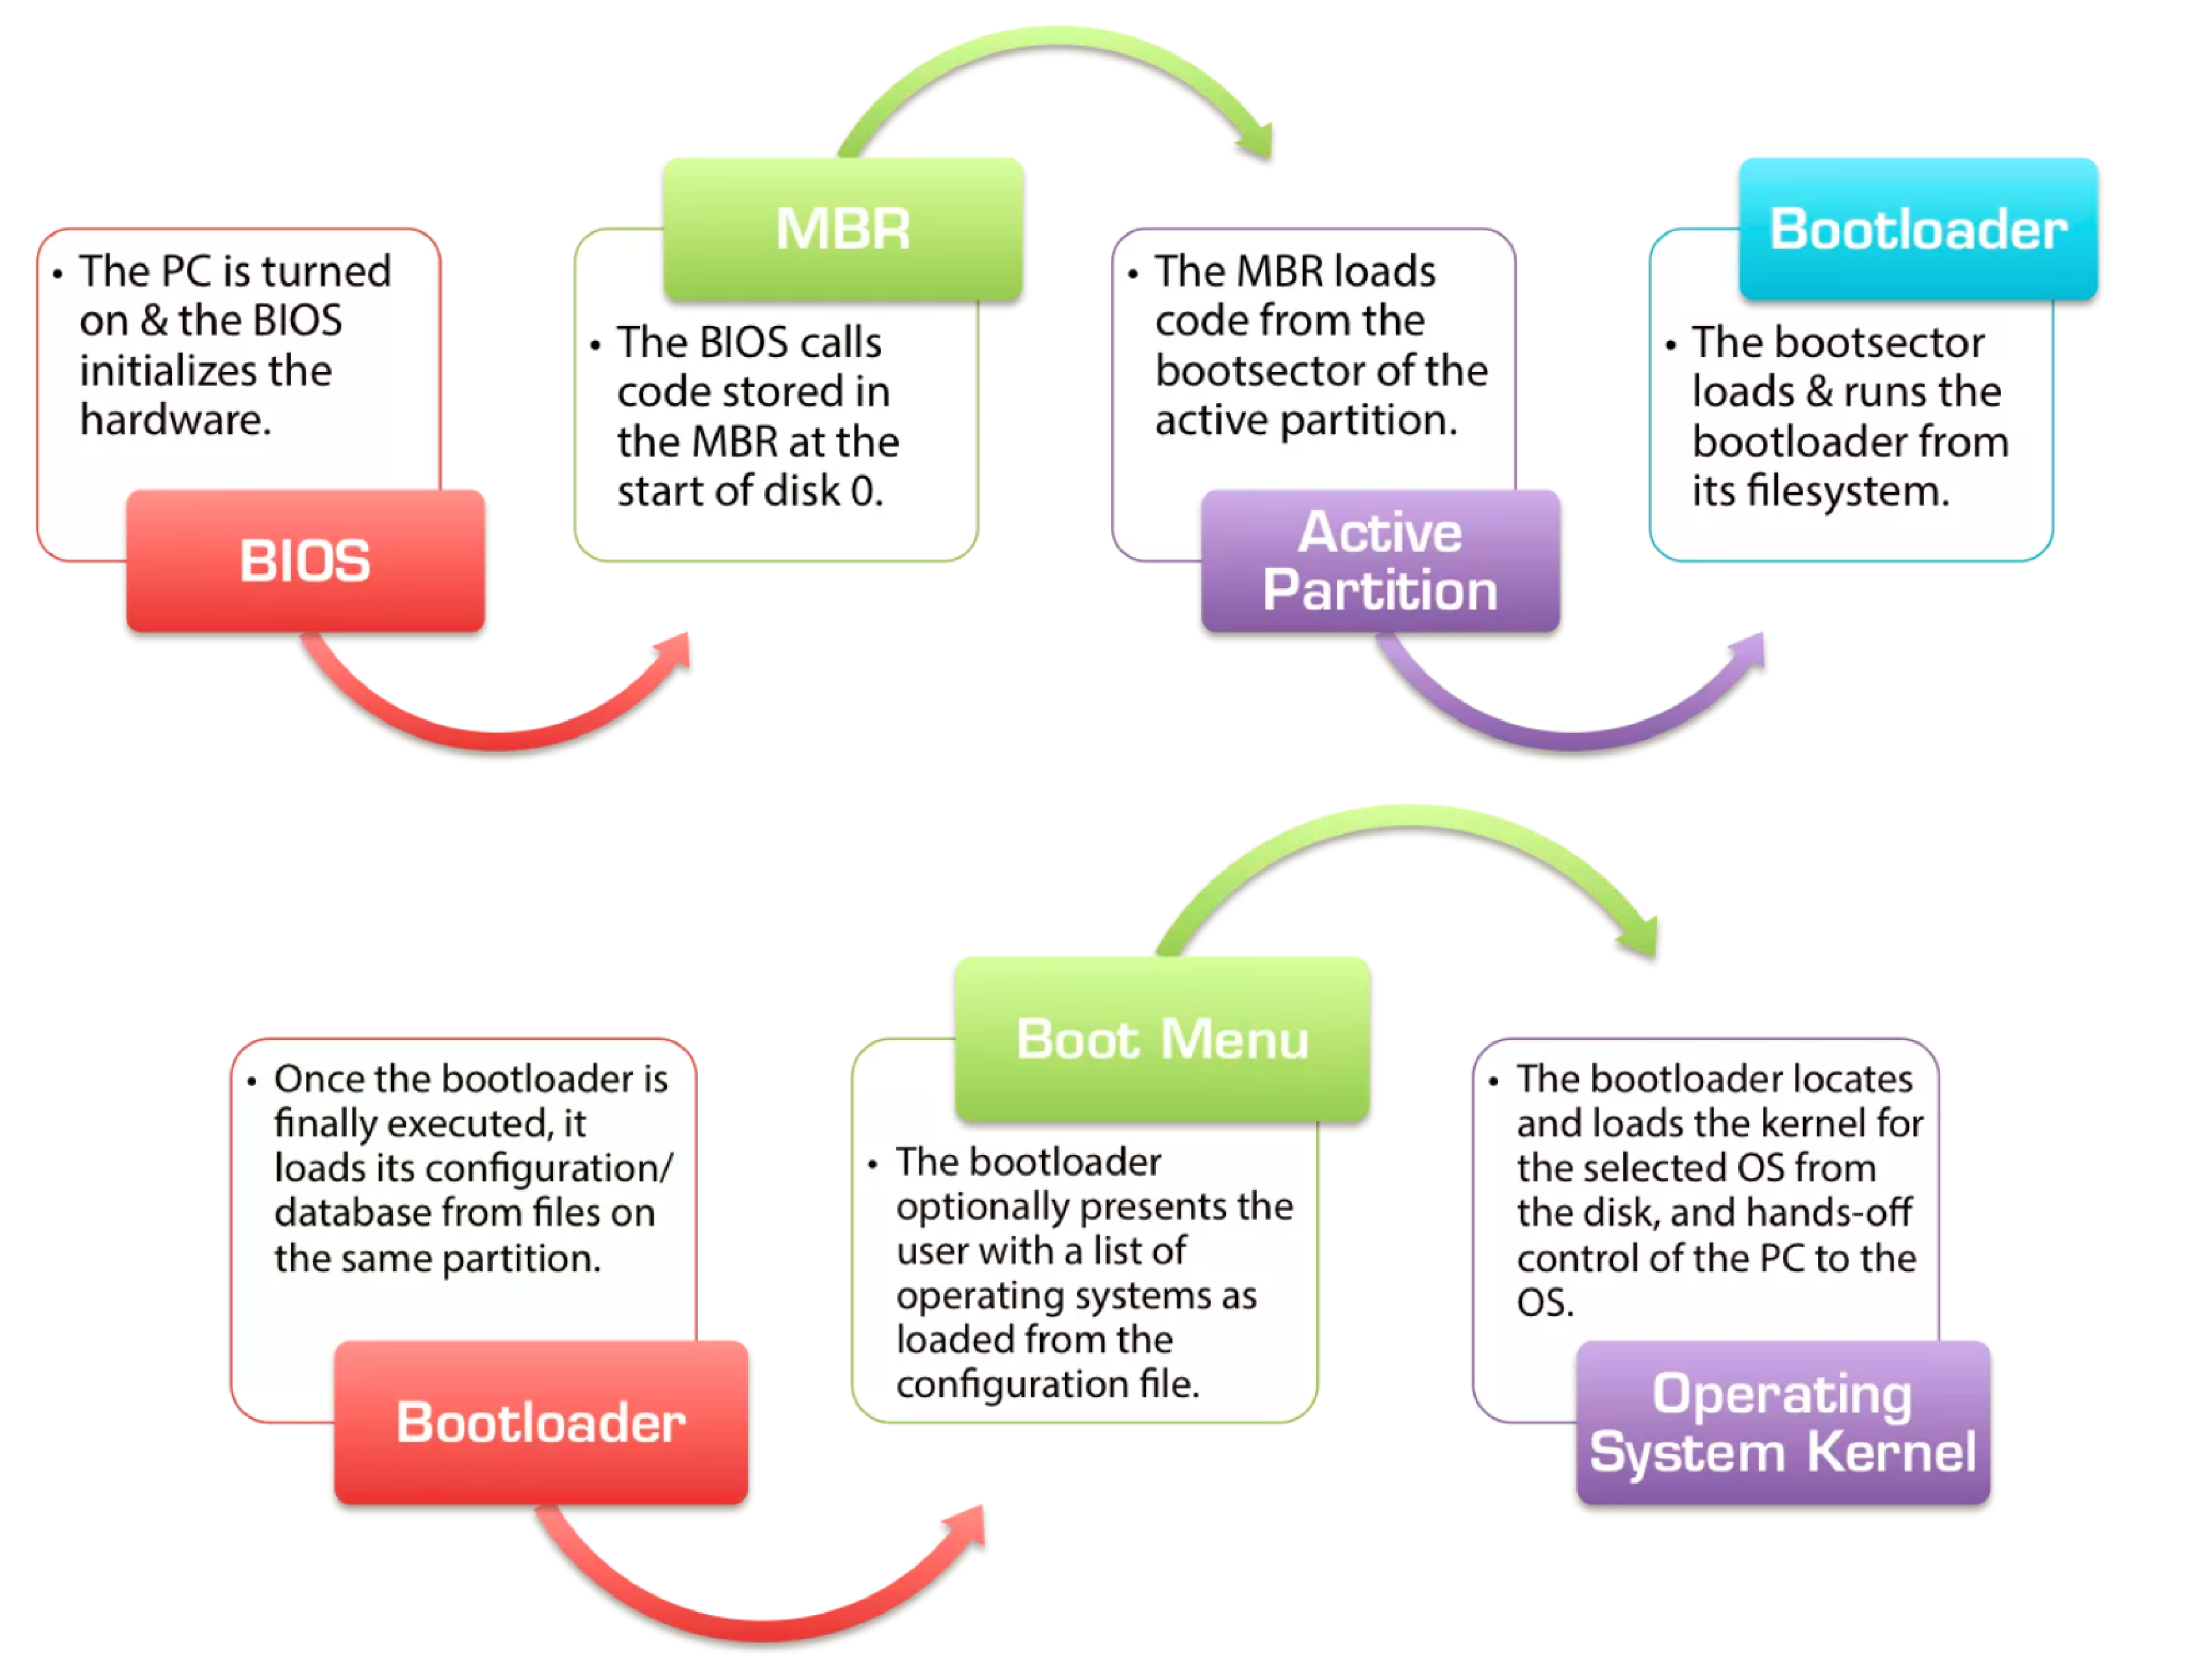
\includegraphics[height=3cm,
  angle=0]{./images/boot-process.eps}}
  \caption{Boot process}
  \label{fig:boot-process}
\end{figure}


\subsection{How a PC boot with BIOS code?}

Fig.\ref{fig:boot-process} shows a boot process is broken down into several
major components, each of which is a completely-separate subsystem with many
different options and variations.

When the power is on, the internal power takes a few moments to generate the
reliable power for the whole computer (motherboard's chipset,
processors). If it is good, the motherboard receives ``Power Good'' signal, and
the central processing unit (i.e. CPU) starts to run.

When you first turn on the machine, there is nothing in the (RAM) memory. Thus,
the processor doesn't really know what to do and where to read.
So, all CPUs are pre-programmed to read and execute a small bit of startup code
(considered as a small simple O/S) called {\bf BIOS code}
(Sect.\ref{sec:BIOS-code}) stored in ROM chip (aka BIOS chip as the BIOS code
resides on the chip associated with the motherboard). This code persistent in
the ROM regardless of power supply or not. This is where hardware meets software
for the first time.


To ensure the computer, regardless of the CPUs, always run. All CPUs are
designed to read at a fixed address in the BIOS - called {\bf reset vector}
right at the end of the system memory (see in frame); and the BIOS code, written
by different motherboard manufacture, needs to be programmed so that at that
address, it contains just a 'JMP' (jump instruction) and the next address
(which is now can be anything depending on the BIOS manufacturer) is the
starting addressof the real BIOS code startup program. At this point, the BIOS
code take over the control, which does a number of tests and device what
operating system to load next (Sect.\ref{sec:BIOS-code}).
\textcolor{red}{Nowadays, BIOS is replaced by a newer system called UEFI}
(Sect.\ref{sec:UEFI_BIOS}).

\begin{mdframed}
As part of the CPU specification (or design), the default location that a CPU
will go to find the first instruction to execute (after a reset) is called a
{\bf reset vector}, and its value is 
\begin{itemize}
  \item \verb!FFFF0h! (for 8086 CPU) is the real-mode saddress in hardware by
  design which is 16 bytes below 1MB.
  
  In segmented address (CS:IP registers): FFFFh:0000h
  
  \item \verb!00FFFF0h! (for 80286 CPU)
  
  In segmented address (CS:IP registers): F0000h:FFF0h
  
  \item \verb!FFFFFFF0h! (for 80386 and later x86 CPU)
  
  In segmented address (CS:IP registers): FFFF0000h:FFF0h
  
\end{itemize}
This address contains the JMP instruction to the next address that the CPU
needs to execute. \textcolor{red}{Both of these addresses (e.g. 0xFFFF0 and
wherever it points to) are typically in ROM}.

\end{mdframed}


\subsection{* BIOS code (Basic Input/Output System)}
\label{sec:BIOS-code}

BIOS code is the code stored in the BIOS chip or ROM chip, originally to be
used as a bootstrap on x86 CPUs. The company which makes the motherboard needs
to write the BIOS code
\begin{itemize}
  \item AMI BIOS
  \item PHOENIX BIOS
  \item AWARD BIOS
\end{itemize}

\begin{mdframed}

Unlike 80486-era machines, the machines run code directly from BIOS, many modern
processors are not designed to run code from BIOS directly. Instead, the BIOS
code is loaded into RAM, and then the processors execute it.
\end{mdframed}

\textcolor{red}{BIOS code is written in?}:
The real BIOS code is called the machine's firmware which was programmed in
assembly. It is a low-level software with a typical UI for user's setting,
Fig.\ref{fig:BIOS_interface}.
Nowadays, the majority of the code in some higher level language that can be
compiled into machine code (mainly in C since 1990s), and leave written in
assembly as few portions of it as possible, preferably only the bootstrapper,
(the very first few hundreds of instructions that the CPU jumps to after a start
/ reset,) and whatever routines deal with specific quirks of the underlying
architecture. The vast majority of the code that makes up a BIOS is specific to
the underlying hardware, so it does not really need to be portable:
it is guaranteed that it will always run on the same type of CPU, mainly x86
architecture.
\url{https://softwareengineering.stackexchange.com/questions/298628/which-language-is-a-bios-written-in}

Most BIOS chip has a region of memory called {\bf boot block} which is not
updatable and run first. What it does it to detect the integrity of the whole
BIOS code (via checksum, hash, \ldots) before jumping to the BIOS code.

{\bf What BIOS code does?}:  The BIOS is made up of two parts: the POST code
(Power-on Self Test - Sect.\ref{sec:POST}) and runtime services
(Sect.\ref{sec:BIOS-runtime-services}).

\subsection{---- POST}
\label{sec:POST}

The job of the POST is to perform a check of the hardware. 
It performs identifying (and possibly testing) available memory, determining
clock speeds, and so on.  If the tests succeed, the machine beeps once. 

Common diagnostics include beep codes (which vary from vendor to vendor) or
diagnostic codes that can be written out to a specific raw address. Some plug-in
cards allow easy access to these codes; the standard solution is that diagnostic
codes are written to port 80. Some manufacturers sell plug-in cards that
display, in hex, whatever byte was last written to port 80.

\url{https://www.ibm.com/developerworks/library/l-bios/}


\subsection{---- BIOS runtime services}
\label{sec:BIOS-runtime-services}

BIOS runtime services does local device enumeration and initialization, proceeds
to look for devices attached to the motherboard (e.g. video card BIOS, search
for other devices that may have their own ROMs)). For \textcolor{red}{warm
boot}, it does POST which if successful, then it does runtime services.

\begin{itemize}
  \item video card BIOS is the BIOS built-in code (normally found at location
  \verb!C000h! in memory), that initialize the video card, e.g. display
  information on the screen about the video card
  
  \item if the device's ROM has its own BIOS code (e.g. floppy device has its
  BIOS code at \verb!0000:7C00!, IDE/ATA hard disk BIOS found at C8000h,
  \ldots), then run it.
  
  \item other tests: memory count, test hardware's normal functioning \item
  display on the screen summary
\end{itemize}

What happens after the BIOS is done with all of this? It finds a chunk of code
somewhere (typically on a disk and must be {\bf bootable}) and runs it,
generally loading an operating system. If the operating system is DOS, or
something similar to it, all of this setup work means that you can pretty much
have your command prompt instantly.

Depending on the setting of what disk containing the bootable O/S to use, the
final part of the BIOS code is to transfer the control to the code on that
device.  Again, to avoid the confusing, the BIOS code read and load the code on
the first sector of that bootable device, and put into the memory location
0000:7C00 addresss. The BIOS's role is over as it transfers control to
0000:7C00.

The code on that first sector of the bootable device can be MBR code or VBR code
(Sect.\ref{sec:VBR-code}). The BIOS does not care whether it is loading a MBR or
a VBR code.
\begin{itemize}
  \item  When booting from a floppy drive, which has no partitioning information
  and therefore no MBR, only the VBR code is effectively loaded into 0000:7C00.

  \item When booting from hard disks, which may have multiple partitions
  (Sect.\ref{sec:partitions-harddisk}) and thus it needs to have MBR region
  and in that region MBR code reside which is the code to tell on what partition
  there is the operating system to load (Sect.\ref{sec:bootable-device-and-MBR}).
    
  If the MBR code is found, it is loaded into memory at locations in the address
  range \verb!0000:7C00! through \verb!0000:7DFF!, then the BIOS calls
  \verb!INT19! (Sect.\ref{sec:INT19}) to jump to the memory location 0000:7C00.
 
In the MBR code, if it detects the VBR code, then the MBR
moves itself to 0000:0600, and then overwrites it's original location
(0000:7C00) with the VBR code.
\url{http://stackoverflow.com/questions/2058690/what-is-significance-of-memory-at-00007c00-to-booting-sequence}
\end{itemize}

\subsection{---- INT19}
\label{sec:INT19}

INT19 is the assembly language statement that the BIOS use to jump to the 
address at which the MBR code is loaded, i.e. so that the operating system can
be loaded. Interrupt 19 reboots the system without clearing memory or restoring
interrupt vector.

\url{http://www.delorie.com/djgpp/doc/rbinter/id/79/22.html} 


\subsection{---- memory-chip to store BIOS code}

The BIOS code is stored on a {\bf {\it non-volatile} read-only-memory (ROM)
chip} of the motherboard (which cannot be modified easily), or, in modern
computers, in the {\bf flash memory chip} (which enable the BIOS chip to be
updatable without removing the chip from the motherboard). However, the second
design allows the modern computer vulnerable to BIOS rootkits.

The flash memory chip is developed from  Electrically Erasable and Programmable ROM
(EEPROM); while the old ROM is called UV-EPROM (which requires erasing with
UV-light exposure before they can be reprogrammed). IMPORTANT:
EEPROM can also be configured so that it cannot be reprogrammed.
\footnote{\url{http://superuser.com/questions/707254/where-is-the-bios-stored}}

\begin{mdframed}

There are two types of flash memory chip which are both non-volatile (i.e. data
retains even when the power is off):
NAND and NOR logic gates.
Unlike UV-EPROM which need to be completely erased before it can be written,
flash memory chip doesn't need so. In NAND flash memory, a block of memory (or
pages which is much smaller than the entire memory) can be deleted and
rewritten. In NOR flash memory, a single machine word (byte) is required to be
deleted and rewritten.

In NAND, there are two types:  Single-Level Cell (SLC) and Multi-Level Cell
(MLC). Each cell can store data, using 1 bit per cell for SLC and 2 bits per
cell for MLC. SLC provides higher performance and more costly. Neverthless, NAND
cells are not designed to last forever, i.e. the cells wear out after each
write (not a problem with reading).

\footnote{\url{http://www.kingston.com/us/community/articledetail/articleid/12?Article-Title=NAND-Flash-Technology-and-Solid-State-Drives-SSDs}}
\end{mdframed}
\vspace{0.2cm}


\textcolor{red}{A motherboard typically has only one or two BIOS chips}. If
there are two, then one is the main one, and the second is the back-up one, just
in case we mess up the main one, e.g. updating the BIOS is not successful. The
location of the BIOS chip is given in Fig.\ref{fig:BIOS_location}. The different
motherboards can use different BIOS chips. The popular BIOS chips are AWARD
BIOS.


% When the machine boots up, the BIOS is the first (and tiny) OS
% to do necessary things; at the end of the code it transfers control to
% the first boot device (hard-disk, CD-ROM, USB, \ldots) which can be configured
% by user in the BIOS or can be selected by user via a menu option.


\begin{figure}[hbt]
  \centerline{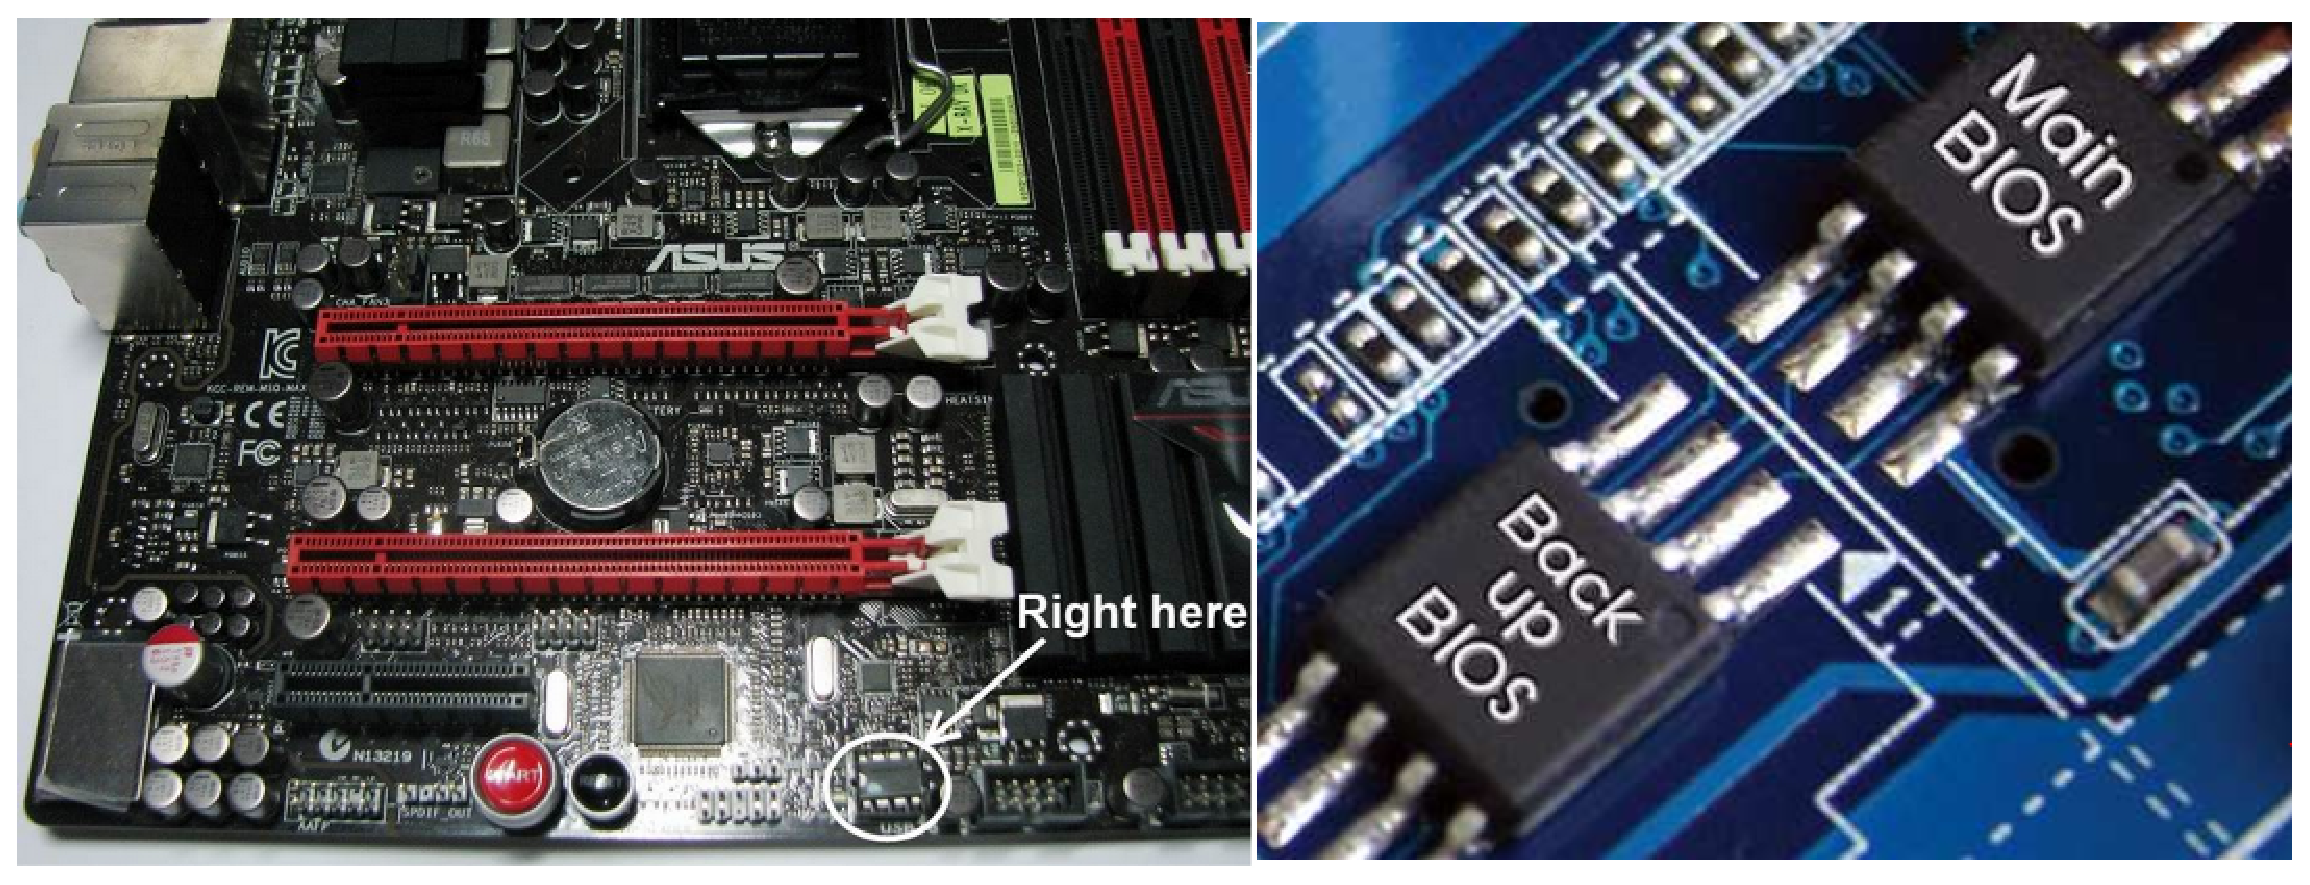
\includegraphics[height=5cm,
    angle=0]{./images/BIOS_location.eps}}
  \caption{(A) BIOS location on the motherboard; (B) two BIOS chips}
  \label{fig:BIOS_location}
\end{figure}



\begin{figure}[hbt]
  \centerline{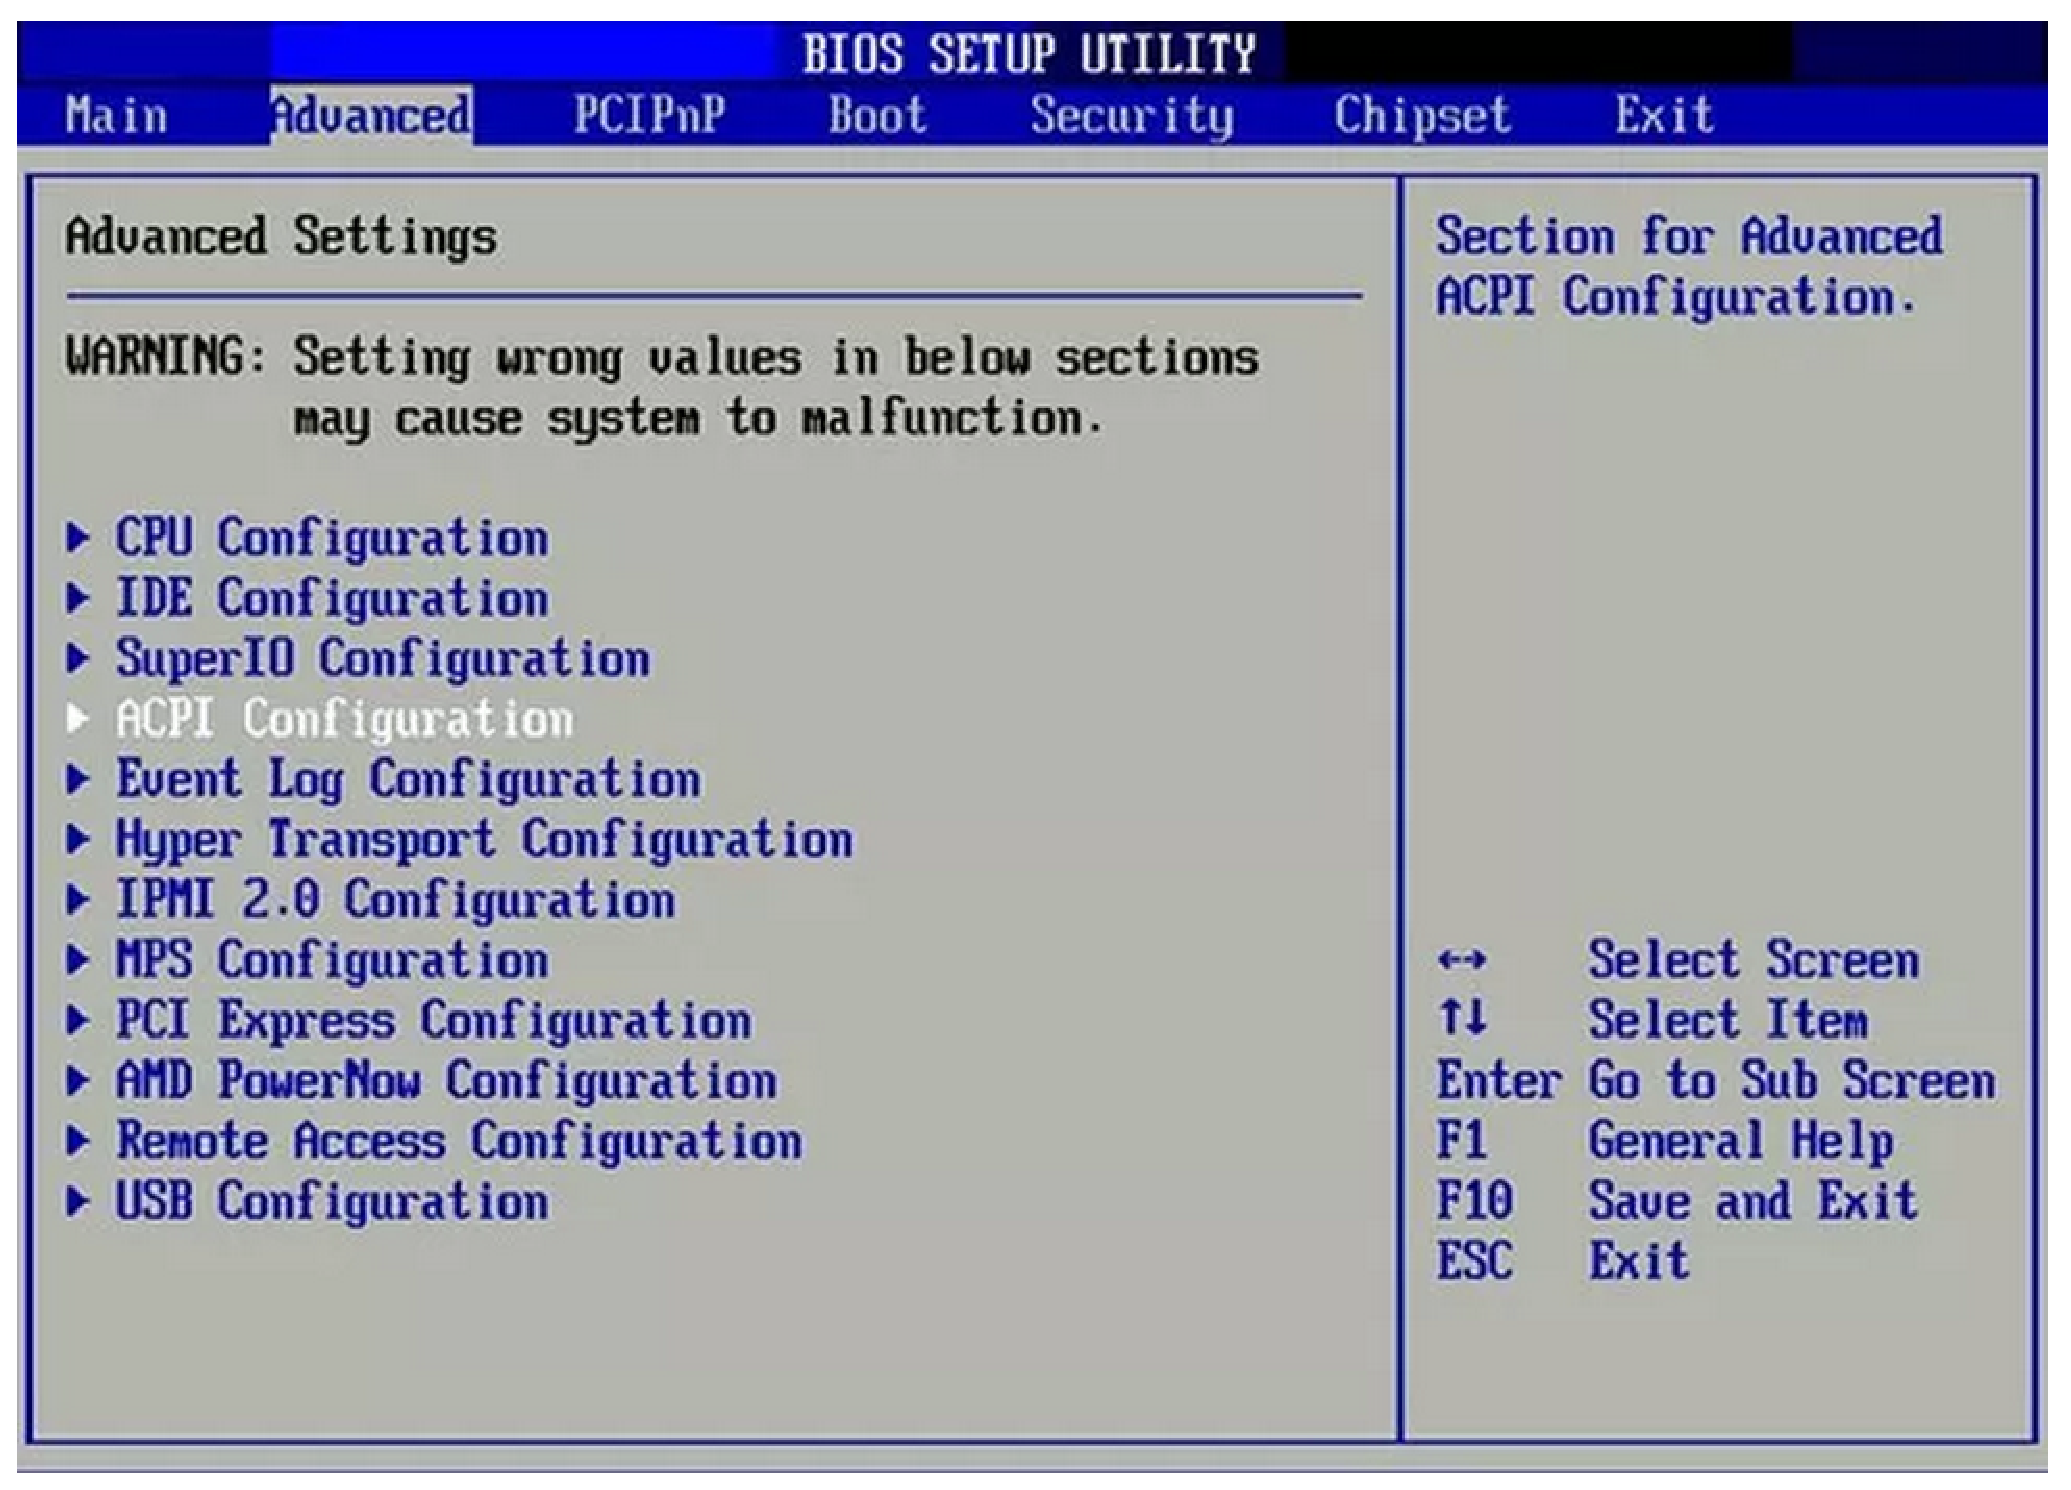
\includegraphics[height=5cm,
    angle=0]{./images/BIOS_interface.eps}}
  \caption{A typical user interface of a BIOS}
  \label{fig:BIOS_interface}
\end{figure}

\subsection{---- from BIOS to UEFI}
\label{sec:UEFI_BIOS}

% As discussed above, BIOS's code or the machine's firmware boots by jumping to
% the exact location (first sector) on the bootable device and execute the code
% from there.
BIOS code was designed to work since Intel 8088 processor which is 16-bit.
Because of that, the early design now comes with several limitations.
\begin{enumerate}
  \item  So, even nowadays, BIOS code is still 16-bit and is limited to 1MB
  addressable space, which means the BIOS code need to be small. 

  \item  In order to load the operating system code, BIOS reads a fixed location
  on the bootable device - the MBR. Inside this MBR contains a small piece of code known
as primary boot loader of 446 bytes, and a region of 64 bytes containing the
information about partitions. This poses several limitations:
\begin{itemize}
  \item maximum 4 primary partitions per disk
  \item limited code size for BIOS
  \item limited code size for primary boot loader
  \item limited size of the bootable disk to 2.2TB.
\end{itemize}
\end{enumerate}

There is the need to extend more code to handle more hardware features.
Extensions was added like ACPI (Advanced Configuration and Power Interface).
However, a better approach is to replace BIOS with a brand new system.

The early specification to overcome BIOS limitation is called EFI specification
(Extensible Firmware Interface) which was first developed by Intel, and the last
version is EFI 1.10 (July 2005).  After EFI 1.10, the Unified EFI forum was formed, and EFI was
renamed to
UEFI.\url{http://www.intel.com/content/www/us/en/architecture-and-technology/unified-extensible-firmware-interface/efi-homepage-general-technology.html}

UEFI replaced EFI; and UEFI specification is managed by Unified EFI Forum. UEFI
2.1 (Jan 2007) supports cryptography, network authentication and user interface
architecture. A typical UI of UEFI has more features and better graphics,
Fig.\ref{fig:UEFI_interface}.

\begin{figure}[hbt]
  \centerline{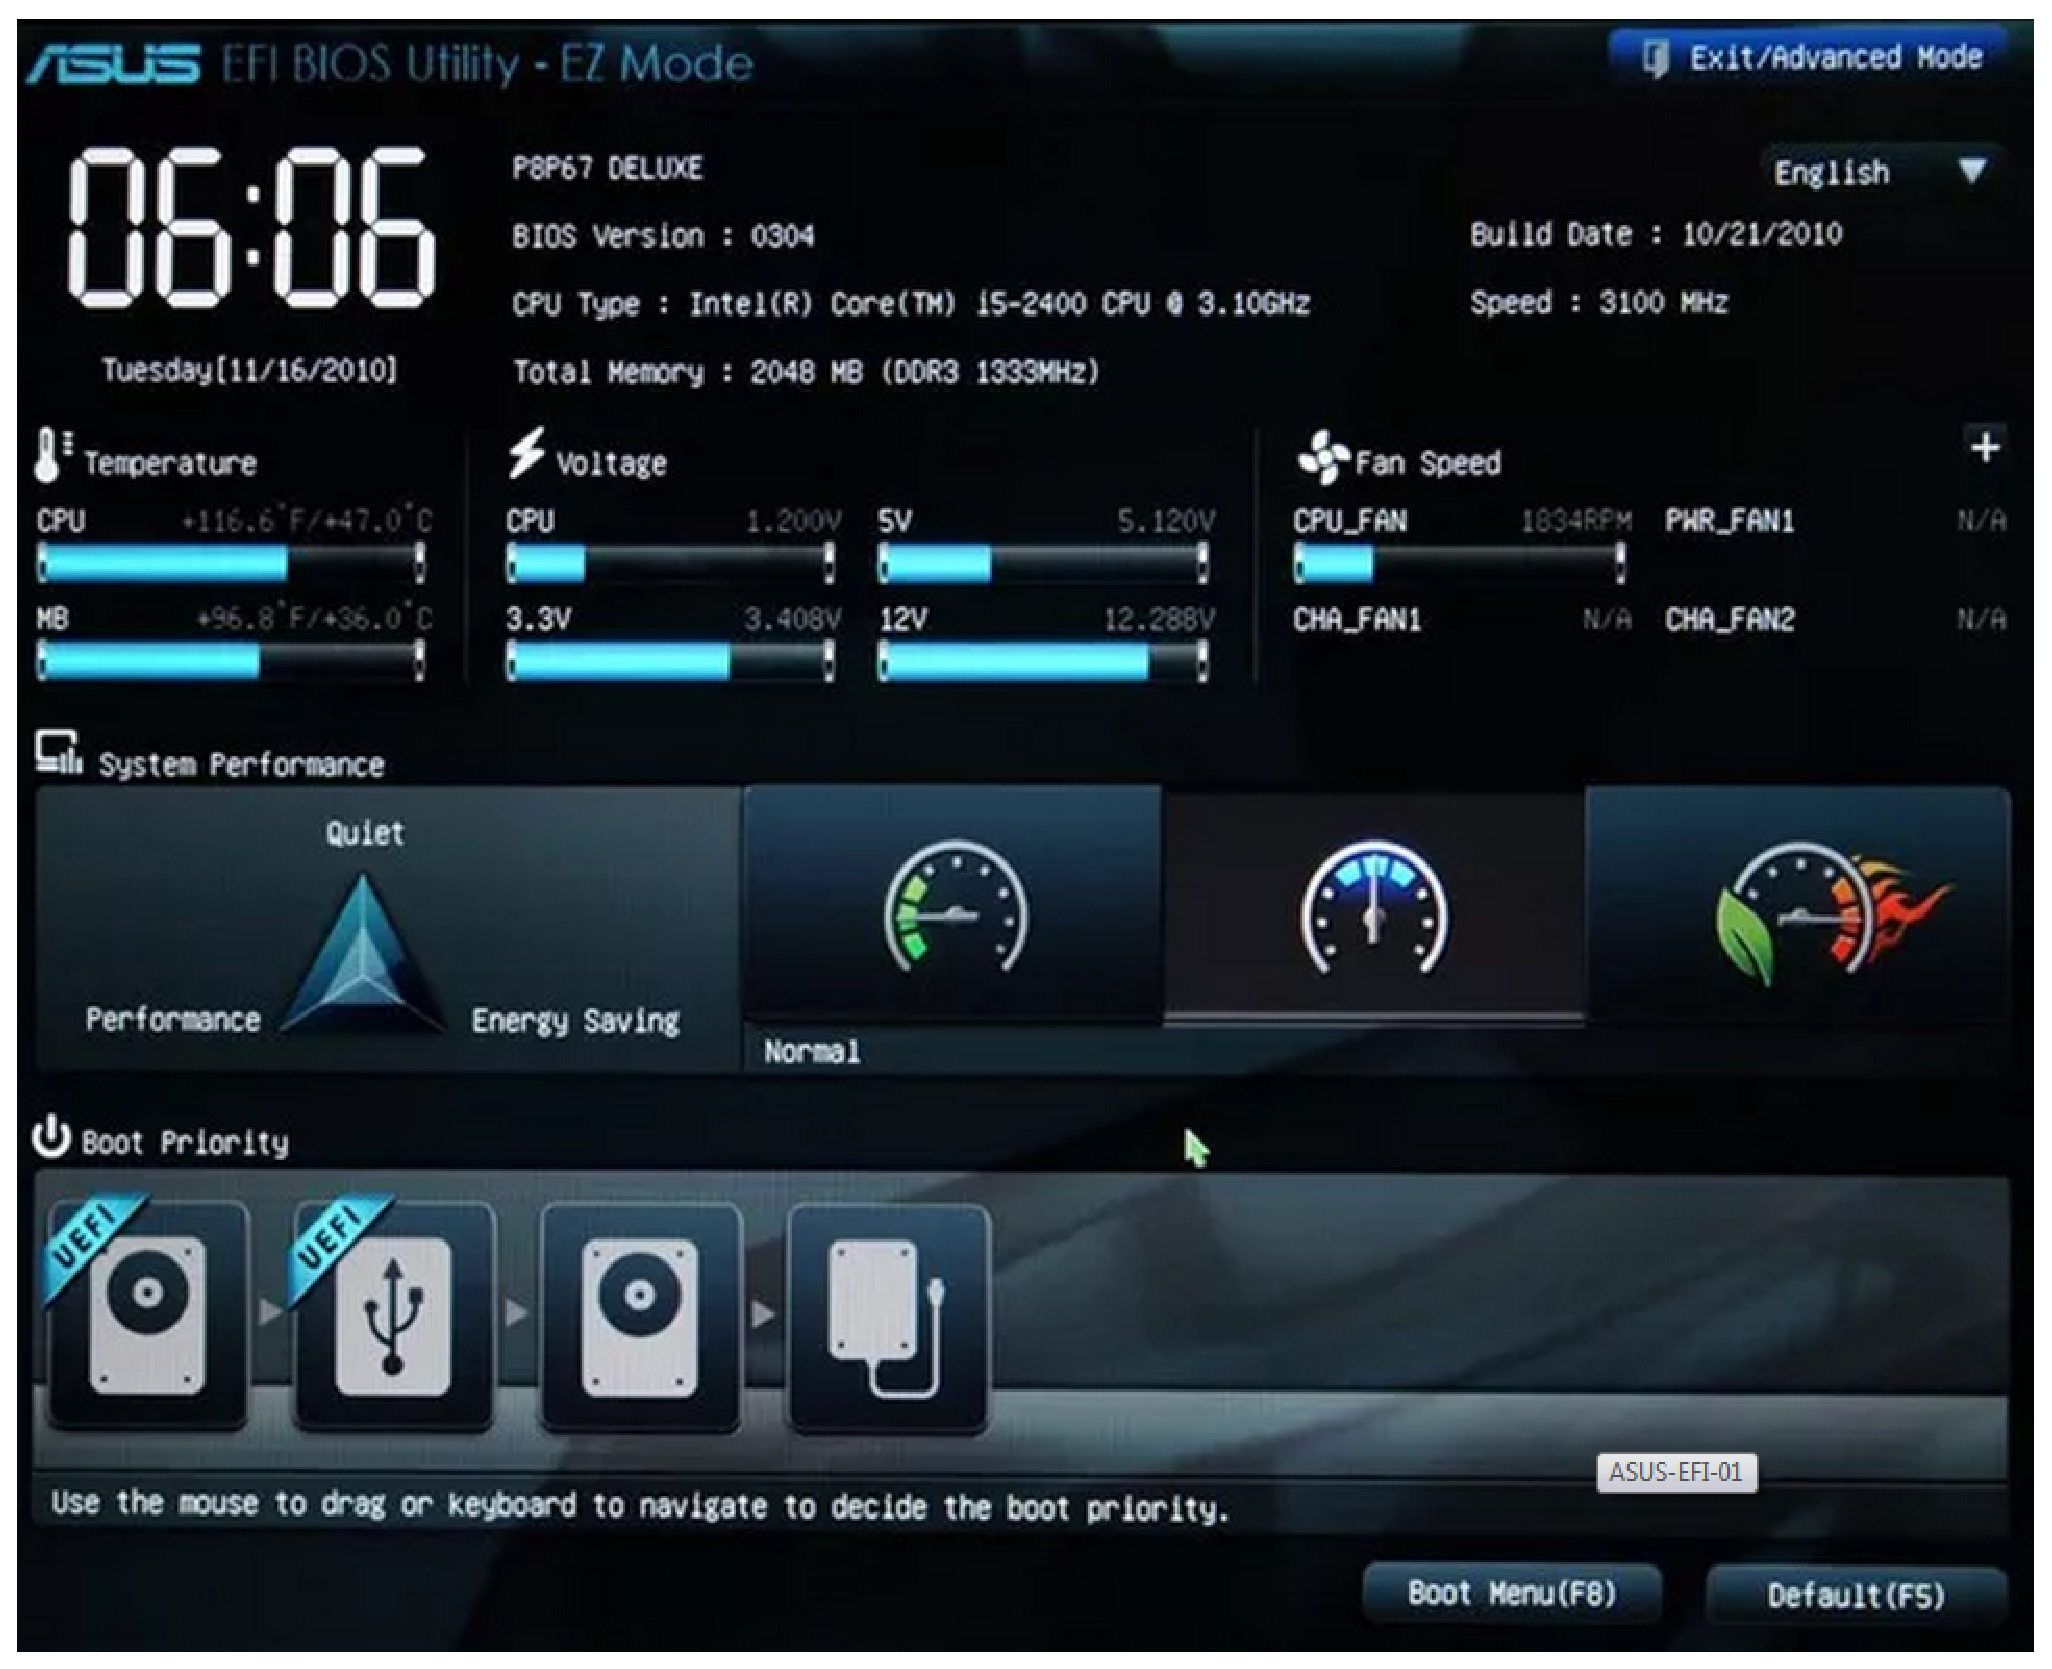
\includegraphics[height=5cm,
    angle=0]{./images/UEFI_interface.eps}}
  \caption{A typical user interface of a UEFI}
  \label{fig:UEFI_interface}
\end{figure}

Why UEFI is better?
\begin{enumerate}
  \item UEFI supports both MBR and GPT. GPT is a new partition scheme, and is
  free from many limitation of MBR (Sect.\ref{sec:GPT}).

UEFI supports booting from disk as large as 9.4 ZB by using GUID Partition Table
(GPT); while BIOS use MBR and less than 2.2 TB disks. 

  \item  UEFI has its own bootloader which can take advantage of EFI boot
  services.

UEFI boots by loading EFI program files (\verb!.efi! extension)
from a partition on a bootable device. This partition is known as ESP (EFI
System Partition). 

O/S boot loaders can also serve as extensions to the UEFI, which itself can
function as a proper boot loader. So, EFI can run Linux kernel directly or use
third-party boot manager like rEFInd, GRUb2 (Sect.\ref{sec:GRUB}) or
\verb!gummiboot! to allow you to select which O/S to boot. From Linux kernel
3.3.0, support for EFI boot loader has been added. UEFI allows more boot
options, doesn't prescribe particular file systems, and has excellent network
booting abilities.

One advantage of using EFI-boot mode is the short initialization time in
hardware, e.g. UEFI on Gigabyte GA-EP45-DS3 initializes in 11 seconds versus
BIOS in 19 seconds. 

  \item  UEFI is CPU-independent architecture and drivers, while BIOS
is specific to x86 processor architecture. 

UEFI uses an architecture-independent byte code format that can be run on
different architectures.

  \item UEFI can use 32-bit or 64-bit; while BIOS relies on 16-bit. 

With 64-bit, it allows the pre-boot program to have direct access to all of the
memory. However, UEFI requires the boot loader to be size-matched, i.e. 64-bit
boot loader if UEFI is 64-bit. Until recently, then
\begin{itemize}
  \item Linux kernel 3.15 (Ubuntu 12.04 LTS use Linux kernel 3.13) support
  booting 64-bit kernel from 32-bit  UEFI firmware running on x86-64 CPUs. This
  requires the UEFI boot loader to support UEFI handover.
\end{itemize}
\url{http://www.howtogeek.com/56958/}

  \item However, the main advantage of UEFI is \verb!Secure Boot! feature (to
  improve security).
  
The problem with BIOS-boot mode is making the system vulnerable to rootkit. To
prevent this, EFI-boot mode require a digital signature of boot loaders. The
current problem is that dual boot is difficult, as it required boot loaders like
GRUB and Linux kernel to be signed.
\end{enumerate}

To check if you have an UEFI-compatible motherboard, open BIOS setting
\begin{verbatim}
UEFI: HL-DT-STDVDRAM GT34N
\end{verbatim}

To check if the system was boot in EFI mode, you can check if the file 
\begin{verbatim}
/sys/firmware/efi
\end{verbatim}  
exists.

\subsection{Volume boot record (VBR) and VBR code}
\label{sec:volume-boot-code}
\label{sec:VBR-code}

The first sector of a data storage device that has not been partitioned, or the
first sector of an individual partition on a data storage device that has been
partitioned (Sect.\ref{sec:partitions-harddisk}) is called {\bf volume boot
record} (VBR). 

Remember that a partition can be formatted in a given filesystem
(Sect.\ref{sec:file-system}). So, the exact layout of the partition will
certainly differ. However, it typically has these 4 parts
\begin{enumerate}
  \item JMP statement (to jump to the exact address on the first instruction of
  the bootstrap code)
  
  \item filesystem header:  contain information specific to and important for
  the filesystem itself.
  
  \item bootstrap code: the next stage of the bootloader process. This code can
  then load the second-stage bootloader (Sect.\ref{sec:secondary-bootloader}).
  
  \item end-of-sector magic value: 0x55 0xAA
  
This is similar to the boot sector in MBR code.
\end{enumerate}

The size of the sector is 512 byte, and the {\it bootstrap code} is the code to
load an operating system (or other standalone program) installed on that device
or within that partition. The code is called the volume boot record code (called
\verb!loader!) and should consume no more than 32KB of memory. If it needs more
memory it should query INT 12h for it, since other pre-boot code (e.g. BIOS
code, MBR code) may still be present elsewhere in memory as well.

The VBR code is either loaded by MBR code (Sect.\ref{sec:MBR-code} - in a
multiple partition disk) or directly by BIOS (in a non-partitioned disk), as
discussed in BIOS section - Sect.\ref{sec:BIOS-runtime-services}). The RAM
memory located where this code is loaded is recommended in the range 0000h:7C00h
to 0000h:FFFFh.

This is the code that can recognize what O/S is available on the given
partition to boot.
To do so, the volume boot code then loads a second-stage bootloader from another location
on the disk (Sect.\ref{sec:secondary-bootloader}). In some boot loaders, VBR
code is part of the multi-stage bootloader, i.e. VBR code will transfer the
control to the secondary bootloader such as LILO and GRUB.

\url{https://en.wikipedia.org/wiki/Volume_boot_record}



\subsection{MBR (primary bootloader)}
\label{sec:MBR}
%\subsection{* MBR of bootable device: primary bootloader + partition table}
\label{sec:bootable-device-and-MBR}
\label{sec:primary-bootloader-MBR}
\label{sec:MBR-code}

Once the BIOS POST and AddOn ROM procedures have completed, the BIOS load the
MBR code and transfer the control to it, Fig.\ref{fig:boot-process}.
The MBR code is aka {\bf primary bootloader}. 

As the device can be divided into different physical and/or logical partitions
(Sect.\ref{sec:partitions-harddisk}), the job of the {\it primary bootloader} is
to find the bootable (or active) partition by looking through the partition
table, once the bootable partition is detected, it scans the remaining
partitions in the table to ensure that they're all inactive. When this is
verified, the active partition's  volume boot code
(Sect.\ref{sec:volume-boot-code}) is read from the device into RAM and executed.
To help BIOS works with different boot loader, i.e. always know the location to
read, it uses the very beginning region of the harddisk, i.e. the first sector.
If the device is a harddrive with multiple partitions
(Sect.\ref{sec:partitions-harddisk}), the first sector is called the Master Boot
Record (MBR).

The first sector (aka {\bf boot sector}), i.e. cylinder 0, head 0, and sector 1
(i.e. offset 0000),  of a data storage device that has been partitioned is
called {\bf Master Boot Record} (MBR). The MBR sector may contain code to locate
the active partition (i.e. the partition that contains the operating system) and
invoke the partition's Volume Boot Record (Sect.\ref{sec:VBR-code}). This MBR
code is usually referred to as a {\it primary boot loader} (and is refer to the
bootstrap code).

% {\bf Master Boot Record} (MBR, master boot sector, boot sector, or partition's
% boot record) occupy the first 512 bytes of the device, starting always at the
% first sector.
% The MBR resides at the first sector of the harddisk; and at the beginning of
% each partition is the {\bf volume boot sector}.

NOTE: If the disk uses a sector size other than 512 bytes, there can be
compatibility issue. A sector size of 4096 results in an eight-fold increase in
the size of a partition that can be defined using MBR, allowing partitions up to
16 TiB (2$^{32} \times 4096$ bytes) in size

The sector is recorgnized as MBR if the last 2 bytes match the magic number (as
given below). If the MBR code (Sect.\ref{sec:MBR-code}) is found and the last
two   bytes (the magic number) is \verb!0xAA55! (i.e. 0x55 followed by 0xAA), or
else the BIOS will treat the drive as unbootable.

SUMMARY: MBR is divided into 2 parts:
\begin{enumerate}
  
  \item first 440-446 bytes: bootstrap code
  
This tiny piece of code is very important. It is called {\bf stage-one
bootloader} or  {\bf primary boot loader} or  {\bf Master Boot Code} (MBC or
primary boot loader). This small  chunk of assembly code that is read by the
BIOS (at the end of the BIOS code) to start the boot process at the given
harddrive. 

What it does is to look-up the partition table, and find the bootable partition,
ask user to select one (if there are multiple bootable partitions), and load the
code from the first sector in that partition - the VBR
(Sect.\ref{sec:VBR-code}).
    
  \item next 64 bytes: {\bf partition table} - Sect.\ref{sec:MPT} which is used
  by the bootstrap code to look for bootable partition.
  
  \item the last 2 bytes: magic number (called the boot sector signature) 
  
    The magic number serves as a validation check of the MBR.
    A bootable partition must have the boot record signature of 
    0xAA55, i.e. 0x55, 0xAA in its last two bytes.
    
\end{enumerate}


The MBR region is where the code called {\bf MBR code} resides. To load VBR
code, the MBR code simply relocate itself to 0000:0600; and then load the VBR
code into 0000:7C00 address.
\begin{verbatim}
0000:7C16 F2            REPNZ                   move MBR from 0000:7c00
0000:7C17 A5            MOVSW                      to 0000:0600
0000:7C18 EA1D060000    JMP     0000:061D       jmp to NEW_LOCATION

        NEW_LOCATION:                        NOW AT 0000:0600
\end{verbatim}
\url{http://www.dewassoc.com/kbase/hard_drives/master_boot_record.htm}

The MBR code then transfers the control to the {\it volume boot code} (boot
program stored in volume boot sector (the first sector) of the active partition) -
Sect.\ref{sec:volume-boot-code}.


\begin{figure}[hbt]
 \centerline{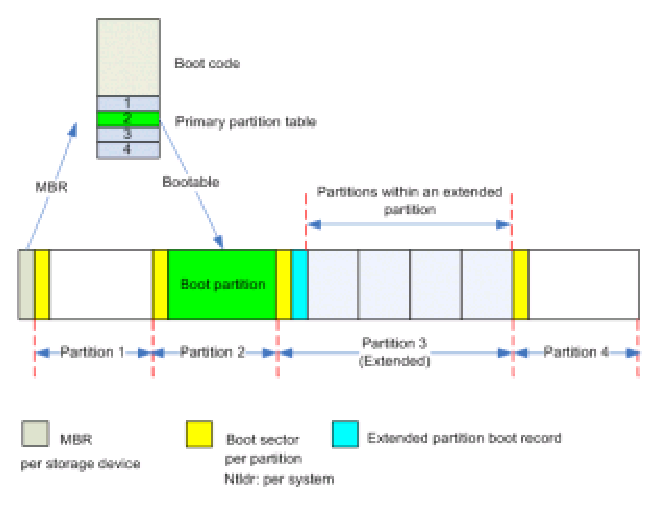
\includegraphics[height=7cm]{./images/harddisk-MBR.eps}}
 \caption{A physical harddrive is divided into 4 partitions}
\label{fig:harddisk-MBR}
\end{figure}

\subsection{* MPT (master partition table)}
\label{sec:MPT}
\label{sec:master-partition-table}

Master Partition Table (MPT): a small bit of code (representing a table) inside
the MBR (Sect.\ref{sec:MBR}).


SUMMARY: MBR messages start at offset 008b; MPT code starts at offset 01be;
and the signature starts at offset 01fe.
\footnote{\url{http://www.ibm.com/developerworks/library/l-linuxboot/fig2.gif}}
\footnote{\url{http://www.dewassoc.com/kbase/hard_drives/master_boot_record.htm}}


MPT contain a complete description of the partitions in the current harddisk.

\subsection{---- classical MPT}

The design of the classical MPT leave enough space to describe maximum four
primary partitions (16 bytes for each partition). If we devide the harddisk into
more than 4, then the other ones must be logical partitions, and is linked to
(or part of) one of the primary partitions.
% In Windows, it supports upto 4 primary partitions (MBR for Windows can only
% recognized maximum 4 - Sect.\ref{sec:MBR-code}), . The
The partition is divided into 3 types, Fig.\ref{fig:harddisk-MBR}
\begin{itemize}
  \item primary partition: maximum 4
  
  To create 6 partitions, to over come this, you need to set one to extended
  partition.
  
  \item extended partition: which functions as a container that allows you to
  create as many logical patitions as you want.
  
  In the extended partitioin: next to the boot sector is the {\bf extended
  partition boot record}, which keeps tract of the many logical partitions you
  create.
  
  \item logical partition: part of the extended partition 
\end{itemize}

There is a flag for each entry that signals if the partition is bootable.

MBR (Master-Boot Record) partitioning scheme allows upto 4 partitions in a disk,
maximum 3 as {\bf primary partitions} and the last one must be {\bf
extended partition} which can then have as many logical partitions. It makes no
difference to install Ubuntu on a primary or logical partition. The default is /
on primary partition and \verb!swap! on as logical partition. Nowadays, most
laptop has a {\bf Recovery Partition} in front of the primary partition.
Recovery Partition is a primary partition but is often hidden to stop people
from modifying it. A partition where you put data is often chosen as a logical
partition.

\subsection{---- advanced active partition (AAP)}

Advanced Active Partitions (AAP) with PTS-DOS 6.60[10] and DR-DOS 7.07) allows 5
partitions.

\subsection{---- AST/NEC MS-DOC and SpeedStor}

AST and NEC MS-DOS 3.x supports 8 partitions.




\subsection{* bootable partition}

A bootable device can be floppy disk, USB, harddrive, CD-ROM; and must contains
MBR code (Sect.\ref{sec:MBR}).

Inside a multiple-partitioned drive, there must be at least one bootable
partition. \textcolor{red}{A bootable partition ({\bf boot partition}) where an
O/S is installed has to be the primary partition}. The first sector in a boot
partition is called {\bf VBR} (Sect.\ref{sec:VBR-code}), and the volume defined
for that boot partition is called {\bf system volume}.

Traditional disk managements in Linux look for which physical disk (/dev/sda,
/dev/sdb) and which partitions are available on these disks (/dev/sda1,
/dev/sda2, etc.).




\subsection{GPT (GUID Partition Table)}
\label{sec:GPT}

GPT (GUID Partition Table) is a standard for a new layout of partition table
(Sect.\ref{sec:MPT}), and is part of UEFI standard to replace BIOS. 
GPT is also used on some BIOS systems because of the limitations of the
partition table in master boot record (MBR). 

GPT is better than MBR (Sect.\ref{sec:MBR}) as GPT supports up to 128 partitions
(by default, and can be increased by running \verb!gdisk!) (while MBR supports
maximum 4) and uses 64-bit pointers. It means GPT can supports disk upto 8 ZiB
(while MBR supports upto 2 TB).

Most GPT data are written twice (at the beginning and at the end of the disk).
This provides a backup in case of data corruption in one place. The damaged data
structures can be detected using checksums which are stored for all important
GPT data structures.

Currently, not all Operating Systems (O/S) are GPT-aware. 
\begin{itemize}
  \item Windows Vista and later support GPT. Yet they can only boot from GPT
  disks with EFI firmware (not BIOS)
\end{itemize}


To partition a disk into GPT, we can use one of the tools
\begin{enumerate}
  \item \verb!fdisk! (version 2.23 and later). Ubuntu 13.10 only have fdisk 2.20
  \item GPT fdisk: it has 3 programs (gdisk, cgdisk, sgdisk)
  \item \verb!libparted!: it supports GPT, MBR, etc. 
\end{enumerate}



\subsection{LUKS partition}
\label{sec:partition-LUKS}

You can get udisks2 to do it for you with udisksctl (available in 14.04 LTS and later):
\begin{verbatim}
// sudo apt-get install udisk
// sudo apt-get install udisk2

udisksctl lock -b /dev/sdXY
\end{verbatim}
where /dev/sdXY is the block device you want to lock (not the LUKS mapper i.e. /dev/mapper/ubuntu)

You can also unlock (open) it with
\begin{verbatim}
udisksctl unlock -b /dev/sdXY
\end{verbatim}

\subsection{Unlock LUKX partition remotely}

\url{https://www.pbworks.net/ubuntu-guide-dropbear-ssh-server-to-unlock-luks-encrypted-pc/}

\subsection{Devices in Unix}

\begin{enumerate}
  \item Floppy disk: /dev/fd[0..9] 
  \item SCSI disk (address-wise): /dev/sd[a\ldots f]
  \item SCSI CD-ROM: /dev/scd0, /dev/sr0
  \item IDE master harddrive: /dev/hda
  \item IDE slave harddrive: /dev/hdb, /dev/hdc
  \item SCSI generic device: /dev/sg0 (used by burning software to access
  writing capability of CD burner drive using ide-scsi layer driver)
  \item SCSI device used for CD-ROM accessing: /dev/scd0
  \item RAMDISK (a portion of RAM being used as a disk drive): /dev/ram0,
  /dev/ram1
  
  We can map this RAMDISK to a folder by first formatting it
  \begin{verbatim}
  ;; as ext2 (default ramdisk size is given in grub.conf)
  ;; ramdisk_size = 16000
  make2fs -m 0 /dev/ram1
  
  ;; or use only 2MB
  make2fs -m 0 -b 2048 /dev/ram1
  \end{verbatim}
  data in this RAMDISK can be accessed faster than from the regular harddrive
  \begin{verbatim}
  mkdir /mnt/rd
  
  mount /dev/ram1 /mnt/rd
  \end{verbatim}
\end{enumerate} 
Partitions on each disk are represented by appending a decimal number to the
disk, e.g. /dev/hda1, /dev/hda2 are the first and second partitions of the
master IDE harddrive. 

The primary partitions are numbered from 1 to 4. From number 5, the partitions
are logical. The extended partition is the primary partition holding the logical
partitions is not usable by itself (apply to both SCSI and IDE). 


In a RAID configuration, the partitions are numbered as /dev/md0, /dev/md1

\section{Secondary Boot Loaders (Bootloader)}
\label{sec:bootloader}
\label{sec:secondary-bootloader}

The secondary boot loader (second-stage bootloader) is known as the bootstrap to
load the real O/S kernel (Windows, Linux, \ldots). It is loaded by the bootstrap
code in the VBR (Sect.\ref{sec:VBR-code}). When people talk about bootloaders
and boot files, they are often referring to this final, critical step of the
boot process.

Once control of the PC has been handed-off from the BIOS to the bootstrap code
in the MBR and from the MBR to the bootstrap code in the partition bootsector,
and from there there to the executable boot files on the active partition, the
actual logic involved in determining which operating system to load by this
secondary bootloader. 

The secondary bootload is a normal file stored amongst other normal files in the
filesystem on the disk; and is not stored at a dedicated offset within the
partition. This significantly more-complicated bootstrap code must actually read
the table-of-contents for the filesystem on the partition.


While the executable bootloader files could theoretically contain hard-coded
information pertaining to the operating systems to be loaded from the disk, that
wouldn't be very useful at all. As such, almost all bootloaders separate the
actual, executable bootloader from the configuration file or database that
contains information about the operating system(s) to load.

There are many different (secondary) bootloaders out there. Also, each operating
system has its own preferred bootloader, specifically designed to read its
filesystem and locate the kernel that needs to be loaded for the OS to run.

When you install an operating system, the default secondary bootloader is also
installed.
\begin{enumerate}
  \item bootloaders for Windows O/S: NTLDR (Sect.\ref{sec:NTLDR}), BOOTMGR
  
  \item bootloaders for Linux O/S
\end{enumerate}

\subsection{Windows bootloaders}
\label{sec:bootloader-Windows}

\begin{itemize}
  \item NTLDR is loaded by VBR code (Sect.\ref{sec:volume-boot-code})
  
  The booting order of NTLDR is given in
  \url{http://dralu.com/wp-content/uploads/2010/08/Boot_Ntldr.png}
  \url{http://dralu.com/?p=275}
  
\end{itemize}

\subsection{* NTLDR}
\label{sec:NTLDR}



\textcolor{red}{\bf Legacy boot system}:
{\bf NTLDR} (NT loader) is the name of the default bootloader used by all
Windows NT O/S, including Windows XP, Windows 2000 and Windows Server 2003.  It
requires, minimum, two files
\begin{verbatim}
ntldr           the main boot loader itself
NTDETECT.COM    a helper program that runs to detect
                hardware and identify services 
                (required for booting NT-based OS)
\end{verbatim}
\url{https://en.wikipedia.org/wiki/NTLDR}


Additional files
\begin{verbatim}
boot.ini      reside on the active partition, e.g. C:\boot.ini
              contains boot configuration (e.g. list of O/S and 
              their locations) 
              (if missing, NTLDR will default to
              <partition>:\Windows on the first partition of the first hard
              drive, e.g. C:\Windows)
\end{verbatim}

The Windows NT kernel image is \verb!ntoskrnl.exe! file
\url{https://en.wikipedia.org/wiki/Ntoskrnl.exe}

Example \verb!boot.ini!
\begin{verbatim}
[boot loader] 
timeout=10 
default=multi(0)disk(0)rdisk(0)partition(4)\WINNT35 

[operating systems] 
multi(0)disk(0)rdisk(0)partition(4)\WINNT35="Windows NT..." 

C:\BOOTSECT.W40 = "Windows 95" /WIN95 
C:\BOOTSECT.DOS = "MS-DOS 6.20" /WIN95DOS 
C:\MBR.LIN = "Linux 1.1.59"
\end{verbatim}
\url{http://www.tburke.net/info/ntldr/ntldr_hacking_guide.htm}

\subsection{* BOOTMGR + winload.exe}
\label{sec:BOOTMGR}


\textcolor{red}{\bf New boot system}: used by Windows Vista, 7, 8 and 19 and
Windows Server 2008. \verb!BOOTMGR! : Windows Boot Manager is for loading the
Windows kernel (Chap.\ref{chap:Windows-kernel}) into RAM.
  
BOOTMGR is self-contained, i.e. no helper program is needed.
The list of O/S(es) is now read from a BCD file in 
\begin{verbatim}
  \boot\BCD             if the legacy BIOS 
                        (of the active partition)

  EFI system partition  if UEFI 
\end{verbatim}

Boot Configuration Data (BCD) file is a firmware-independent database for
boot-time configuration data to replace the previous \verb!boot.ini! file. Boot
Configuration Data may be altered using a command-line tool (bcdedit.exe), using
Registry Editor (regedit.exe), using Windows Management
Instrumentation, or with third-party tools such as EasyBCD, BOOTICE, or Visual
BCD Editor.
  
Once loaded, \verb!BOOTMGR! invoke either 
\begin{itemize}
    \item \verb!winload.exe! (BIOS) or \verb!winload.efi! (UEFI) for fresh
    boot. The file is located in \verb!\windows\system32\!
  
    \item \verb!winresume.exe! (BIOS) or \verb!winresume.efi! (UEFI) for
    resuming from hibernate. The file is located in \verb!\windows\system32!
  
\end{itemize}
  
{\bf In the new system}, there are more choice for boot options
\url{https://en.wikipedia.org/wiki/Windows_Vista_startup_process}


\subsection{Linux bootloaders}
\label{sec:bootloader-Linux}

The list of open source bootloaders that can recognize Linux-kernel is given in
Fig.\ref{fig:Linux-bootloaders}.

Unlike NTLDR second-stage bootloader in Windows, many bootloaders in Linux are 
first- and second-stage boot loaders combined, such as LILO
(Sect.\ref{sec:LILO}), and GRUB (Sect.\ref{sec:GRUB}).

For embedded platforms, read Sect.\ref{sec:bootstrap-loader-os}

\begin{figure}[hbt]
  \centerline{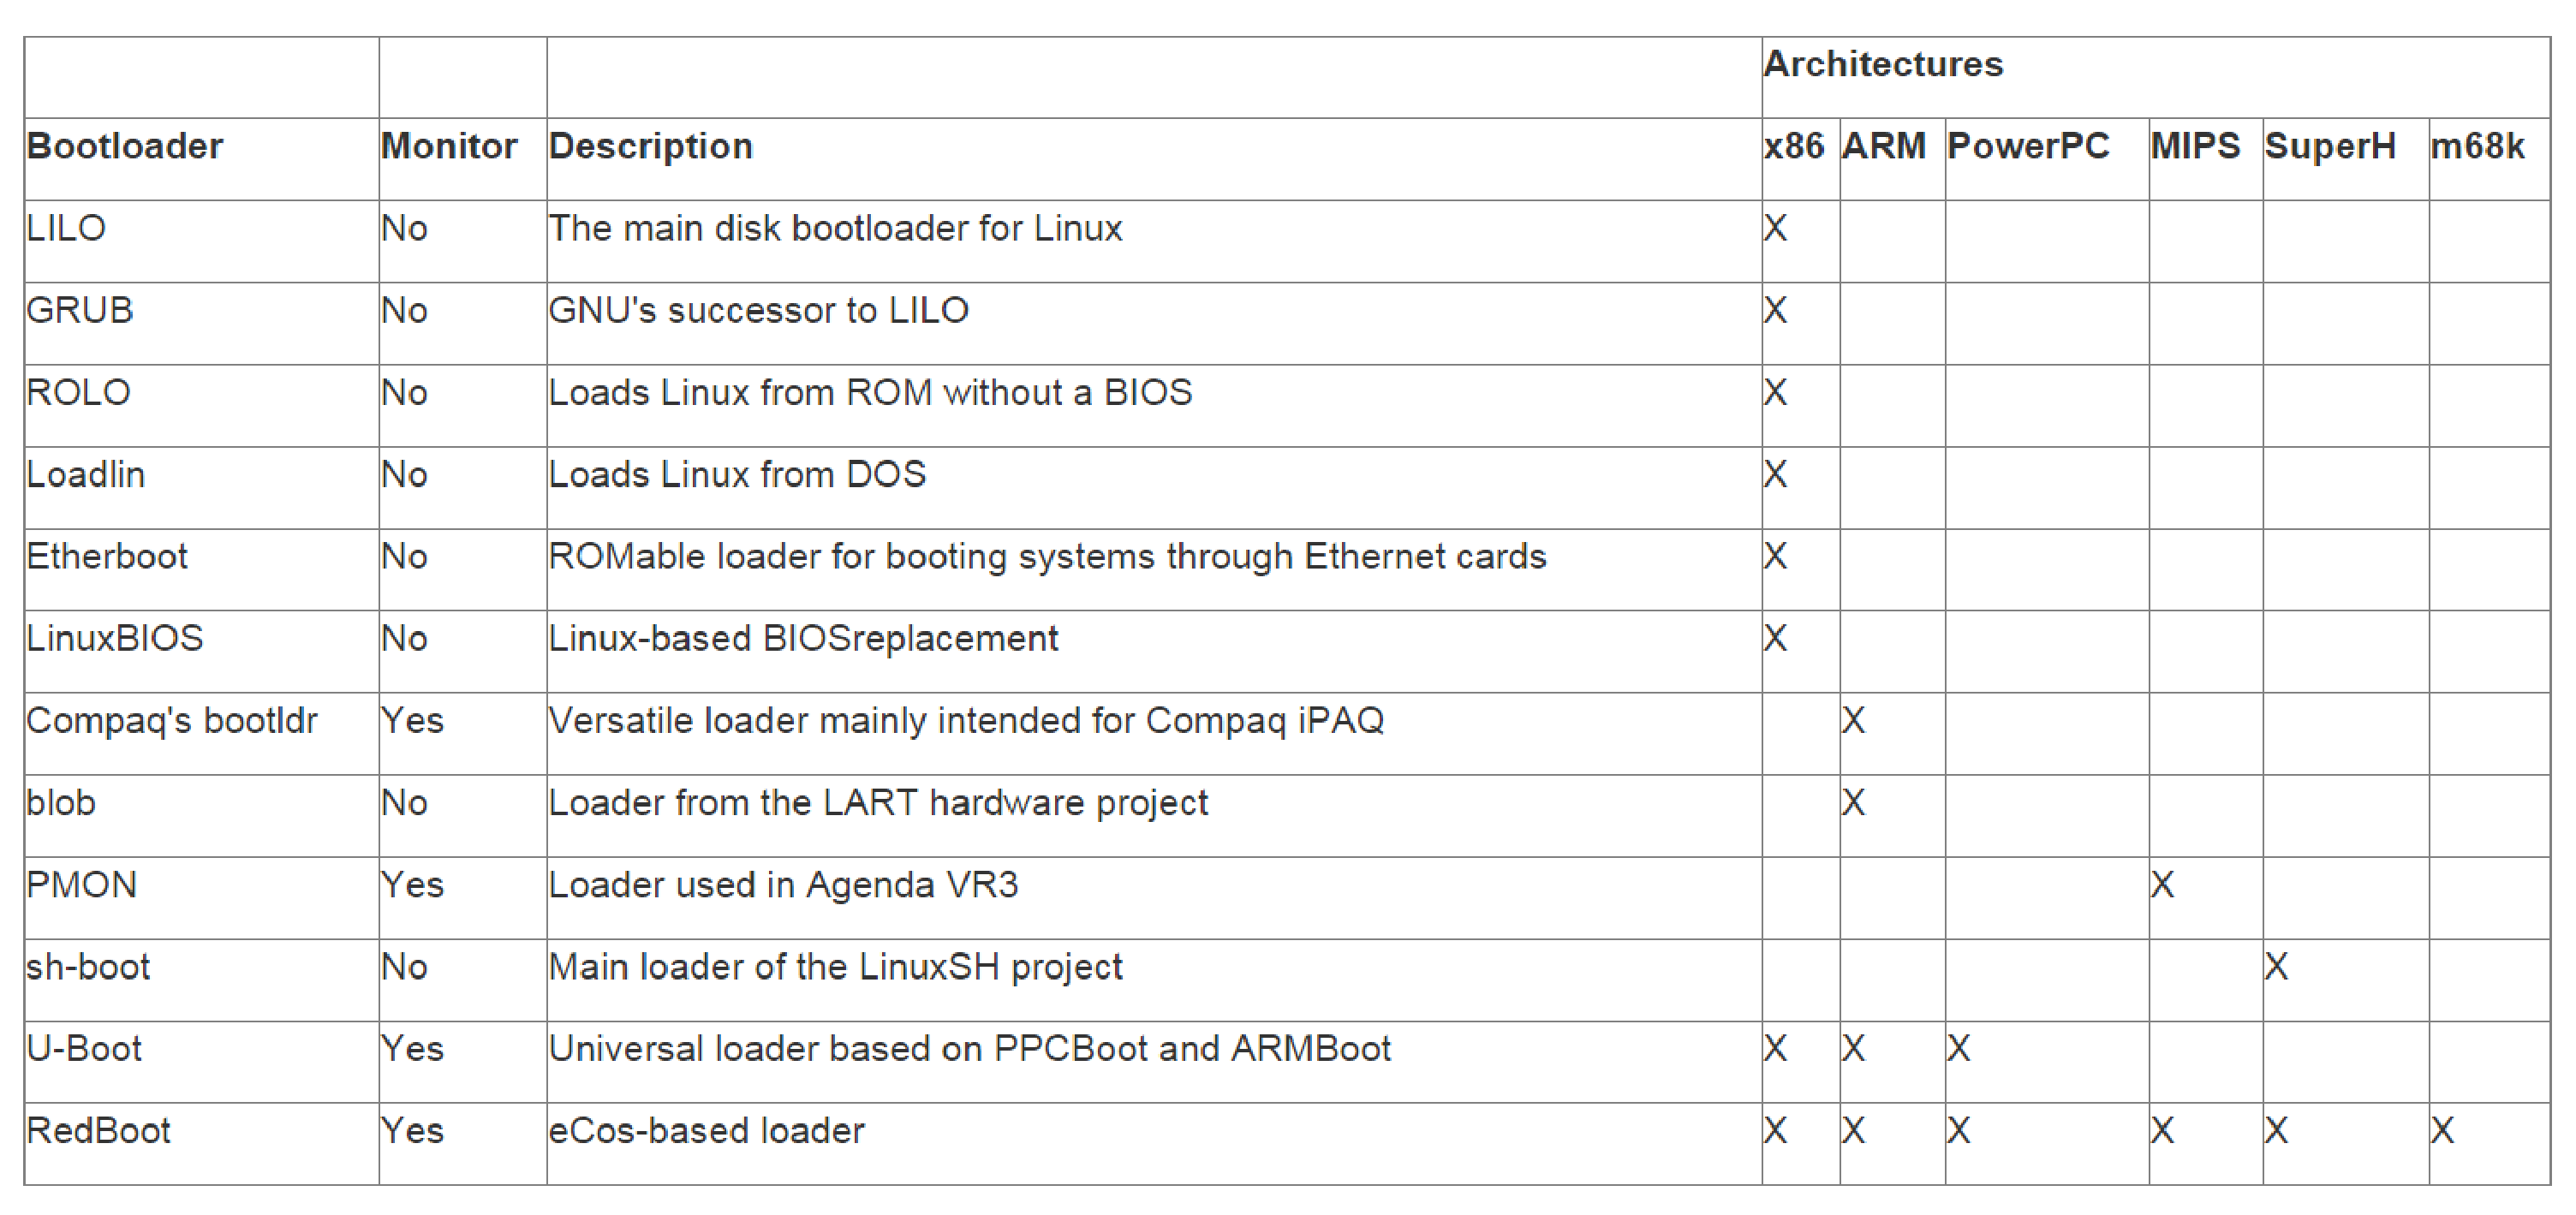
\includegraphics[height=5cm,
    angle=0]{./images/Linux-bootloaders.eps}}
\caption{Linux-capable open-source bootloaders}
%http://etutorials.org/Linux+systems/embedded+linux+systems/Chapter+9.+Setting+Up+the+Bootloader/9.1+Bootloaders+Galore/
\label{fig:Linux-bootloaders}
\end{figure}

\url{http://etutorials.org/Linux+systems/embedded+linux+systems/Chapter+9.+Setting+Up+the+Bootloader/9.1+Bootloaders+Galore/}

\subsection{* LILO}
\label{sec:LILO}

The information for booting is saved in \verb!/etc/lilo.conf! file
\begin{verbatim}
image = /boot/vmlinuz-custom-2.6.37.6
  root = /dev/sda1
  initrd = /boot/initrd.gz
  label = newkernel
  read-only # Non-UMSDOS filesystems should be mounted read-only for checking
  append = "hdc=ide-scsi"
  
\end{verbatim}

If you have multiple images, then you can use
\begin{verbatim}
  prompt
  timeout=50 
  compact
  vga=extended
  linear
image = /boot/vmlinuz-custom-2.6.37.6
  root = /dev/sda1
  initrd = /boot/initrd.gz
  label = newkernel
  read-only # Non-UMSDOS filesystems should be mounted read-only for checking
  append = "hdc=ide-scsi"

image = /boot/vmlinuz2
  root = /dev/sda2
  initrd = /boot/initrd.gz
  label = newkernel

\end{verbatim}

Finally, run \verb!lilo! to do the actual update of the boot loader

NOTE:
\begin{itemize}
  \item \verb!image=! path to Linux kernel image
  \item \verb!root=! path to real RFS (can be omitted if we have root=current
  in the global section)
  \item \verb!initrd=! path to initrd image (optional, can be omitted if we
  don't use initrd)
  \item \verb!label=! text to name the kernel
  \item \verb!append=! a string containg kernel parameters
  \item \verb!read-only! : a flag indicating the RFS is mounted as read-only

  \item \verb!Linear!: a BIOS trick, often necessary but can make SCSI disk
  non-portable to a different machine, i.e. you need to rerun \verb!lilo!
  command when you move your SCSI disk to a different computer.
\end{itemize}

\subsection{* eLILO}
\label{sec:eLILO}


\subsection{* GRUB}
% \section{Grub boots}
\label{sec:GRUB}


REMEMBER: While GRUB eventually won out over Lilo and eLilo, it was replaced
with GRUB 2 around 2002, and the old GRUB was officially renamed 'Legacy GRUB.'
Confusingly, GRUB 2 is now officially called GRUB, while the old GRUB has
officially been relegated to the name of 'Legacy GRUB,'.

Unlike Windows-based second-stage bootloaders
(Sect.\ref{sec:bootloader-Windows}), Linux-based bootloader is a multi-stage and
can be used from stage-1, i.e. right after BIOS code,
Fig.\ref{fig:GRUB-process}.


GRUB (Grand Unified Bootloader) is specifically designed for Linux O/S so
it has knowledge of Linux file systems. GRUB is a multi-stage bootloader.

\begin{itemize}
  \item stage 1 = code resides in MBR (limit 512 bytes), with the primary goal
  is to locate the code to run stage 1.5 (if present; otherwise it loads
  stage 2), and load it into RAM. The location: \verb!/boot/grub/stage1!
  
  \item stage 1.5 bootloader (optional) = code that understands the particular
  file system containing the Linux kernel image. The location, for example
  \verb!/boot/grub/e2fs_stage1_5!
  
  \verb!reiserfs_stage1_5! code (to load from a Reiser journaling file system)
  or \verb!e2fs_stage1_5! code (to load from an ext2 or ext3 file system).
  
  GRUB optionally installs stage1.5 when there is room for it. It installs it by
  embedding it in a usually unused area of the hard drive known as the DOS
  compatibility region. It's an area about 30K in size immediately after the
  MBR
  
  \item stage 2 = this is the code that helps in booting of O/S.
  
  In this second stage, a  splash screen is commonly displayed with a list of
  available kernels (defined in \verb!/etc/grub.conf! file, and soft-links from
  \verb!/etc/grub/menu.lst! and \verb!/etc/grub.conf!), and Linux and an
  optional initial RAM disk (temporary root file system) are loaded into memory.
  
  Once the selected kernel image and \verb!initrd! image are loaded into
  memory, the stage 2 boot loader invokes the kernel image
  (Sect.\ref{sec:boot-process-Linux-kernel}).
\end{itemize}

So, GRUB can hold more data (20-30 KB), rather than only 512byte with MBR. GRUB
legacy (version 0.97) is known as GRUB; and since v1.98 it is called GRUB2
(Sect.\ref{sec:GRUB2}). To check version
\begin{verbatim}
grub-install -v
\end{verbatim}


If the first partition of the first harddrive will be the Grub partition
(hd0,0), then you boot with the Live-CD, get to the Grub prompt, and type
\begin{verbatim}
sudo grub

root (hd0,0)     // change to whatever you want the grub partition to locate
                 // hd0 = the first harddisk, 0 = the first partition
setup (hd0)      // where to setup the MBR, match with above
quit
\end{verbatim}

To show GRUB2 menu during boot, we hold SHIFT key during boot (or ESC key in
some cases).

\subsection{---- GRUB legacy (version 0.97)}
\label{sec:GRUB1}

The \verb!/boot/grub! directory contains the stage1, stage1.5, and stage2 boot
loaders, as well as a number of alternate loaders (for example, CR-ROMs use the
\verb!iso9660_stage_1_5!).

\textcolor{red}{Single kernel}: The config file is \verb!/boot/grub/grub.conf! 
\begin{verbatim}
title Red Hat Linux (2.4.20-8)
        root (hd0,0)
        kernel /boot/vmlinuz-2.4.20-8 ro root=/dev/hda1 hdc=ide-scsi
        initrd /boot/initrd-2.4.20-8.img
\end{verbatim}
Explain:
\begin{itemize}
  \item \verb!title <the kernel-string>!
  
  \item \verb!root (disk,partition)! where the RFS is stored
  
  The disks and partitions are numbered by bus numbers, rather then by letters:
  (hd0,0) means /dev/hda1.
  This should points to the partition that contains \verb!/boot/..!
  
  NOTE: \verb!root=LABEL=/! : RedHat/Fedora prefers 'labeling' the partition
  and refers to them thisway.  You can label your partitions any way you like,
  or not at all, with the command \verb!e2label!. But make sure you edit Grub
  accordingly.
\begin{verbatim}
e2label /dev/hdx newlabel

  # print the current label
$ e2label /dev/hda7
$ /

e2label /dev/hda2 FC1-top
\end{verbatim}  
then you can use \verb!root=/dev/hda2! or \verb!root=LABEL=FC-top!.

\url{http://www.linuxforums.org/forum/red-hat-fedora-linux/23010-root-label-grub-conf.html}

  \item \verb!kernel </path/to/kernel-image> [kernel-parameters]!
  
  \verb!ro! = read-only,
  \verb!root=/path/to/real-RFS!,
  \verb!hdc=ide-scsi! (other kernel parameters)
  
  \item \verb!initrd </path/to/initrd-image>!
\end{itemize}
\url{http://www.haifux.org/lectures/88-sil/kernel-compilation.html}

\textcolor{red}{Multiple kernel versions}: A good case is to make an entry for
the backup \verb!initrd/initramfs! (Sect.\ref{sec:initramfs}) in case of kernel's
initrd/initramfs error.
The config file is \verb!/boot/grub/grub.conf!

\begin{verbatim}
title Red Hat Linux (2.4.20-8)
        root (hd0,0)
        kernel /boot/vmlinuz-2.4.20-8 ro root=/dev/hda1 hdc=ide-scsi
        initrd /boot/initrd-2.4.20-8.img

title Red Hat Linux (2.4.20-8) - old initrd
        root (hd0,0)
        kernel /boot/vmlinuz-2.4.20-8 ro root=/dev/hda1 hdc=ide-scsi
        initrd /boot/initrd-2.4.20-8.img.bak

\end{verbatim}


\textcolor{red}{Install GRUB natively}: At the GRUB command-line interface

\begin{verbatim}
root (hd0,0)
   set the GRUB's root device to the first partition (0) of the harddrive (hd0)
   containing the boot directory
find /boot/grub/stage1
   return the information you need for 'root' command
   
setup (hd0)
   install the GRUB bootloader on MBR of the drive (hd0)
   or
setup (hd0,0)
   install the GRUB bootloader into the boot sector of the first partition (0)
   of the drive (hd0)      
\end{verbatim}
If you install GRUB not on the first partition of the first drive, it means
that GRUB cannot be called directly, and then you need to chain-load GRUB from
another boot loader.

\textcolor{red}{Install GRUB using grub-install}:
\url{http://www.gnu.org/software/grub/manual/legacy/grub.html}

With GRUB legacy (Ubuntu 9.04 and earlier): you can easily modify the file
\verb!/boot/grub/menu.lst!. 

  \begin{verbatim}
  ## default 0
  default saved
  
  ## savedefault=false
  savedefault=true
  \end{verbatim}
  save the file and then run 
  \begin{verbatim}
  sudo updage-grub	
  \end{verbatim}
  then the entry we choose in the next time the machine started, it will become
  the default for future starts, until you explicitly choose another one.

Some informations GRUB needs:
\begin{enumerate}
  \item the device and partition, e.g. (hd0,1) : the bracket () is important. hd
  = hard-disk, fd=floppy-disk, cd=cd-rom. first number = device number (zero-based), second number =
  partition index (zero-based)
  
  GRUB make no difference between IDE and SCSI hard-drive, or between primary
  and extended (logical) partitions. Typically, primary partion is marked with
  second number from 0 to 3.
  
  \item the OS on that partition: look at /boot/grub/menu.lst
  \begin{verbatim}
  default 0 # first entry in boot loader list
  timeout 8 # timeout (in second) for boot loader to automatically choose one
  
  # string that help you recognize the OS
  title Windows XP
  # where to find the configuration (hd0,2)/boot/grub 
  root (hd0,2)
  
  # version of OS kernel to use
  kernel /boot/vmlinuz-...
    # if it's not the same device, then 
  #kernel (hd0,1)/boot/vmlinux-...
  
  # temporary files for boot up preperation
  initrd /boot/initrd.img-...
  #initrd (hd0,5)/boot/initrd.img-...
  \end{verbatim}
\end{enumerate}  

Example: NOTE: Windows cannot be boot directly, it use chainloaders, e.g.
\verb!chainloader (hd0,0)+1!. GRUB passes the control of boot sequence to
another bootloader.

\begin{verbatim}
title Windows 95/98/NT/2000
root (hd0,0)
makeactive
chainloader +1
# NOTE: 'makeactive' sets the active partion (hd0,0) as GRUB root device.
#     So, we don't need to specify it again in 'chainloader'

title Linux
root (hd0,1)
kernel /vmlinuz root=/dev/hda3 ro
\end{verbatim}

\url{http://www.dedoimedo.com/computers/grub.html}

\subsection{---- GRUB2 (or modern GRUB v1.98+)}
\label{sec:GRUB2}

GRUB2 is the complete rewritten of existing GRUB - GRUB legacy. GRUB2 (v1.98) is
the default in Ubuntu 9.10. GRUB2 (v1.99) is the default in Ubuntu 11.04 with
some major changes in the Grub file content.

The actual bootloader file for GRUB 2 is called {\bf core.img}.
The GRUB 2 configuration file is more of a (shell) script and less of
traditional configuration file, i.e. it now accepts functions.
The functionality of GRUB 2 is extensible, i.e. with modules,
normally found in a subdirectory of the \verb!/boot/grub/! directory.
Because the configuration file is a regular file on a given filesystem, the
bootloader needs to to be able to read the content of such filesystem.

This leads to a multiple stages, Fig.\ref{fig:GRUB-process}.
\begin{enumerate}
  \item {\bf Initiate filesystem access}: 
  
As GRUB needs to read contents from regular files, GRUb must first load and run
the primitive filesystem "drivers" that give it the ability to read, at the very
least, the filesystem it is located on.
The code that provides this functionality must be compiled into the core
bootloader file itself.

  \item 
\end{enumerate}

 bootloader must also obtain information about the underlying machine hardware
(either via the BIOS or on its own) in order to correctly load the desired
operating system from the correct partition and provide any additional files or
data that might be needed.  


\url{https://neosmart.net/wiki/mbr-boot-process/}

\begin{figure}[hbt]
  \centerline{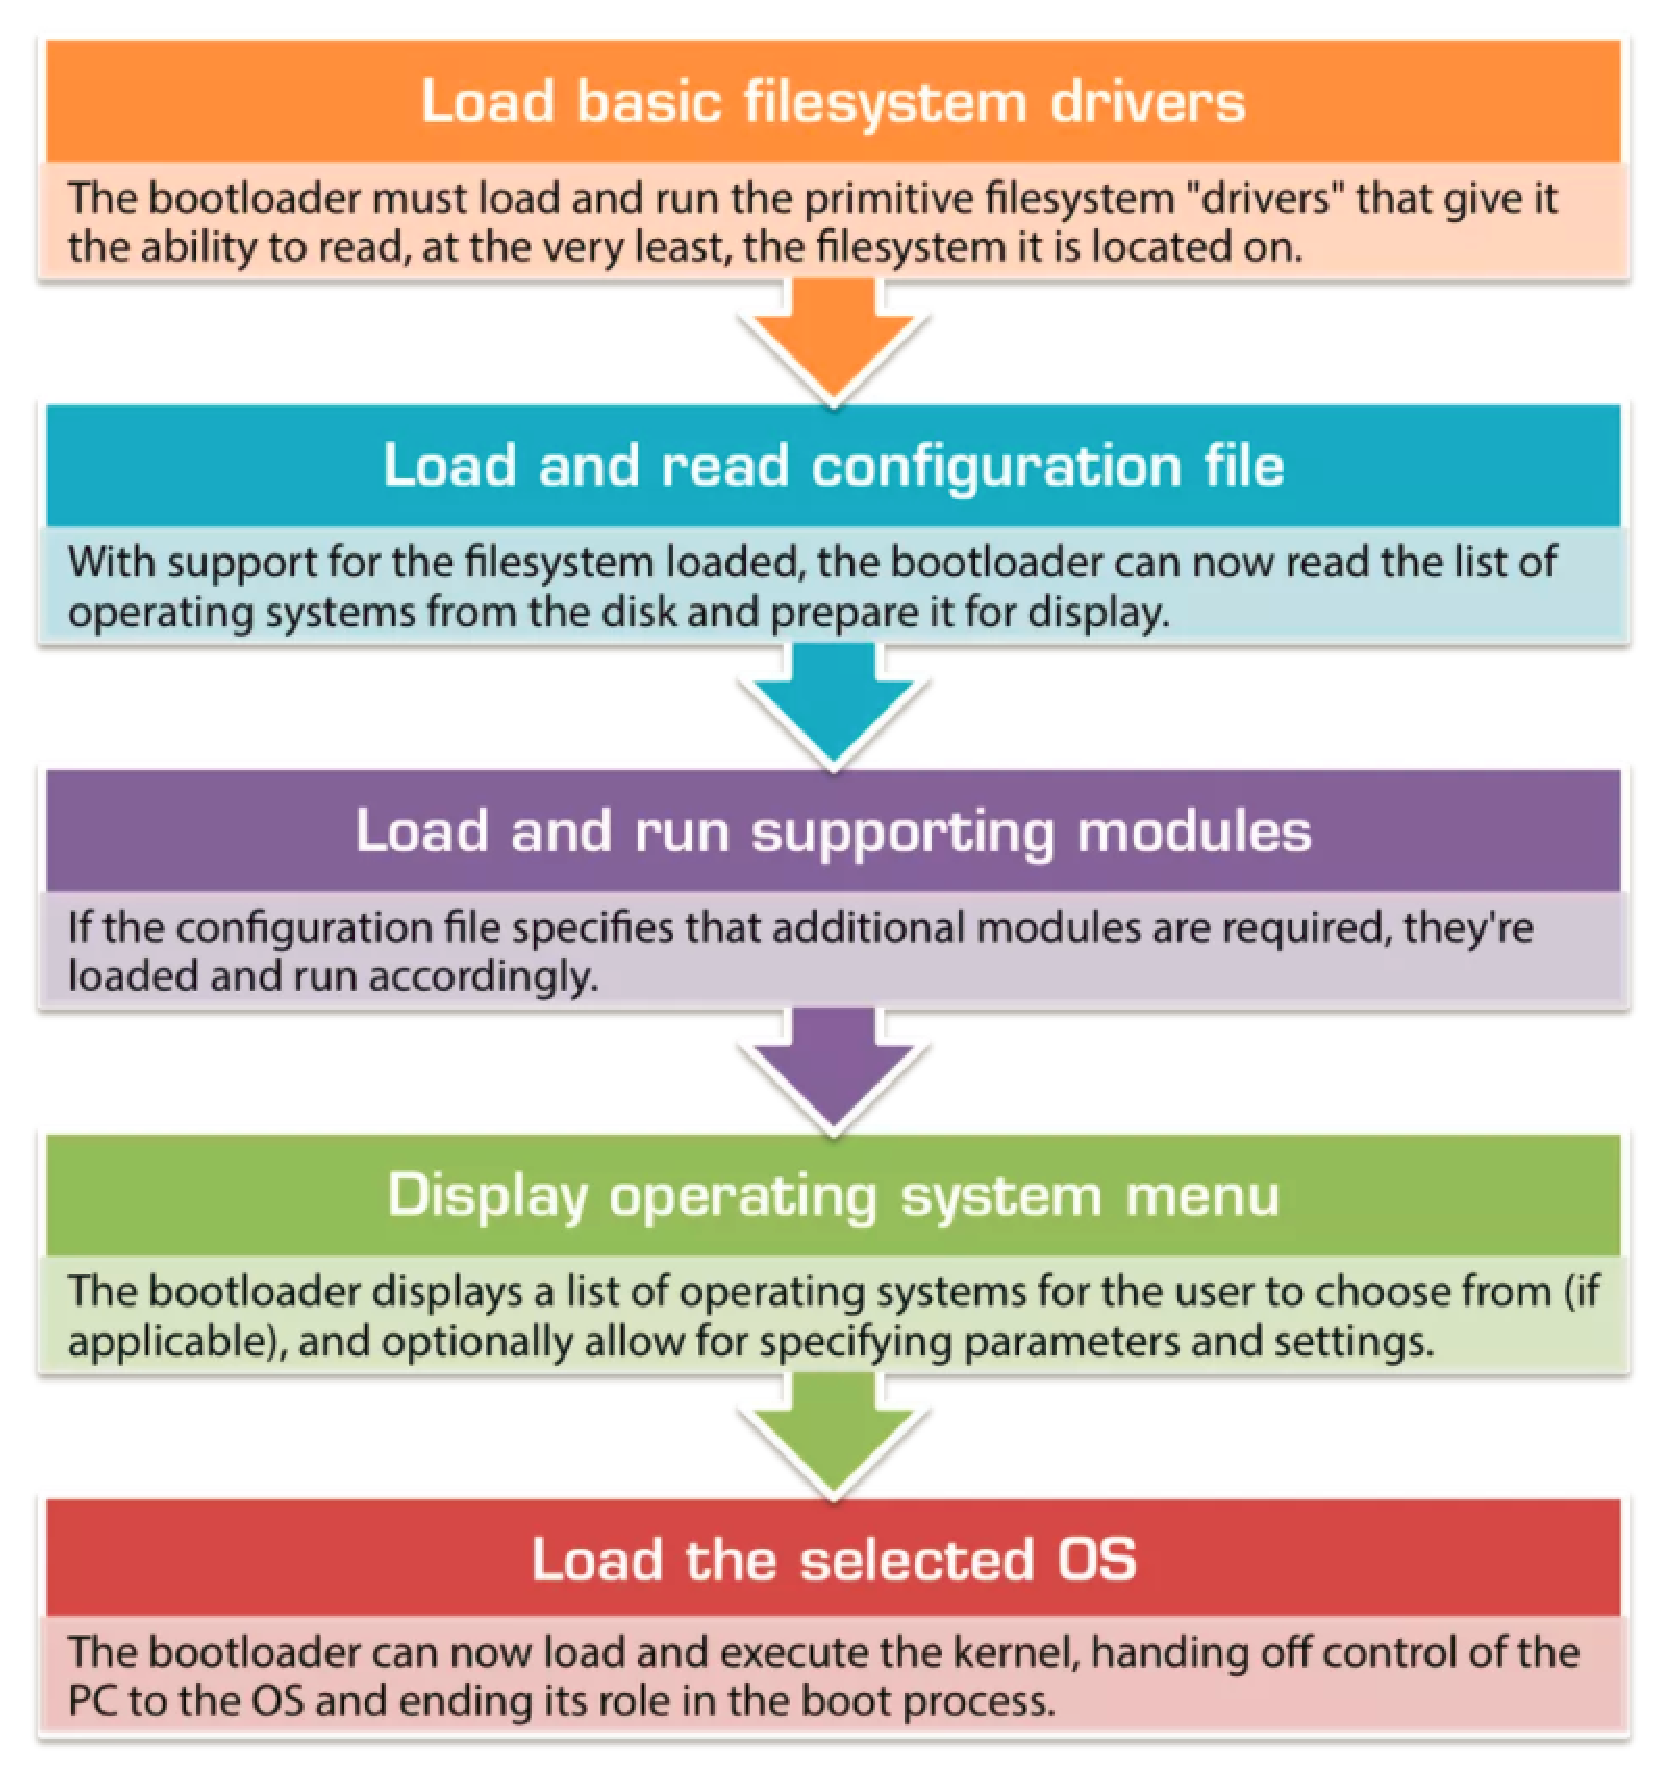
\includegraphics[height=5cm,
  angle=0]{./images/GRUB-process.eps}}
  \caption{Scheme of Component Interactions}
  \label{fig:GRUB-process}
\end{figure}

The main difference between GRUB legacy (GRUB) and GRUB (GRUB2):
\begin{enumerate}

  \item Showing the boot menu is skipped by default. To display it, during boot,
  press and hold (right) SHIFT key (or press ESCAPE key in certain cases)
  
  \item In GRUB, partition is numbered starting with zero, i.e. based on
  (PartionIndex - 1). In GRUB2, partition is numbered as itself.
  \begin{verbatim}
                GRUB         GRUB2
  /dev/hda1 - (hd0,0)        (hd0,1)
  /dev/hda4 - (hd0,3)        (hd0,4) 
  \end{verbatim}
  
  \item GRUB2 has replaced \verb!/boot/grub/menu.lst! by /boot/grub/grub.cfg.
  
  The content of the file is auto-generated, i.e. the list of available O/S
  should be detected automatically, not as given by user. Thus, the content of
  this file is genereted by the machines, and thus should not be modified
  manually.
  
  You can modify this file, but they will be overwritten once you run
  \verb!update-grub! command. This command generate a new file using the
  contents from the files in
  \begin{verbatim}
  /etc/grub.d/*
  /etc/default/grub
  \end{verbatim}
  
  NOTE: To change menu display settings, e.g. timeout, can be
  adjusted by updating file \verb!/etc/default/grub!.
  If you want to change GRUB2 boot entries, we need to modify the templates
  (different shell scripts) in \verb!/etc/grub.d/!, e.g.

\begin{enumerate}
  \item \verb!00_header! : scripts that load GRUB setting from
  /etc/default/grub, i.e. timeout, default boot entry\ldots
  
  \item \verb!05_debian_theme! : define background, color, and themes.
  
  \item \verb!10_linux! : load the menu entries	(where we can modify to
  add/remove boot entries), you can
  add/remove or adjust the number to change the order.
  
  \item \verb!20_memtest86+!: memtest utility
  \item \verb!30_os-prober!: script that scan the hard-disk for OS and add them.
  
  To disable it
  \begin{verbatim}
run this: sudo chmod -x /etc/grub.d/30_os-prober
change GRUB_DISABLE_OS_PROBER='true' in /etc/default/grub
  \end{verbatim}
  
  \item \verb!40_custom!: you can modify to add new entries
\end{enumerate}

  \item  When a kernel is added or remove, we run \verb!update-grub2! command as
  sudo.
   
\end{enumerate}

Users can add customed entries to /etc/grub/grub.conf by creating a custome
file in /etc/grub.d, e.g. \verb!40_custom! file. Once you make some change
(e.g. new UUID of the partitions), you must run

\begin{itemize}
  \item \verb!update-grub2! (for old GRUB2) or
  \item \verb!grub-mkconfig! or \verb!update-grub! (new GRUB2) 
\end{itemize}
to update grub.cfg.



\subsubsection{New/Delete entry}
\label{sec:GRUB2_newentry}

An unused entry can be easily removed by running update \verb!update-grub!.
User-entries (added to \verb!40_custom!) will not be overriden by call to
update-grub. 

ADD NEW ENTRY: To add a new entry to GRUB2 boot menu, we can
use\footnote{\url{http://linux.koolsolutions.com/2009/10/01/info-grub2-101-class/}}
\begin{enumerate}
  \item use \verb!os-prober! and update-grub: add new entry (automatically
  detected) to the end, and the respective entries into the file
  /etc/grub.d/30\_os-prober
  \begin{verbatim}
  apt-get install os-prober
  os-prober
  update-grub
  \end{verbatim}
NOTE: os-prober doesn't detect OS not installed into /boot directory (e.g. puppy
Linux), as it looks for OS information in /boot directory.  
  
  \item edit the file /etc/grub.d/40\_custom
  \begin{verbatim}
#! /bin/sh -e
echo "Adding Windows" >&2
cat << EOF
menuentry "
Windows XP" {
set root=(hd0,1)
chainloader +1
}
EOF
  \end{verbatim}
  and run update-grub.
\end{enumerate}


CHANGE DEFAULT KERNEL: With GRUB2 (Ubuntu 9.10 and
  later)\footnote{\url{http://ubuntuforums.org/showthread.php?t=1195275}}: we
  can modify the file /etc/default/grub, and change \verb!GRUB_DEFAULT=0! to an
  index of the entry in the GRUB boot menu we want to use (NOTE: 0 is the first
  entry). 
  \begin{verbatim}
GRUB_DEFAULT=0
GRUB_HIDDEN_TIMEOUT=0
GRUB_HIDDEN_TIMEOUT_QUIET=true
GRUB_TIMEOUT=10
GRUB_DISTRIBUTOR=`lsb_release -i -s 2> /dev/null || echo Debian`
GRUB_CMDLINE_LINUX_DEFAULT="quiet"
###GRUB_CMDLINE_LINUX=" vga=792"
GRUB_CMDLINE_LINUX=""
  \end{verbatim}
After that, we need to run
\verb!update-grub!\footnote{\url{http://machine-cycle.blogspot.com/2010/01/selecting-default-kernel-to-boot-grub2.html}}
Typically, the boot menu is hidden, if we want it to display (for user to
choose the entry to book), we comment out \verb!GRUB_HIDDEN_TIMEOUT! and set
\verb!GRUB_TIMEOUT! to a value in second. 
\begin{verbatim}
#GRUB_HIDDEN_TIMEOUT=0
GRUB_HIDDEN_TIMEOUT_QUIET=true
GRUB_TIMEOUT=10
\end{verbatim}
  
  
  
  Reference:
  \begin{enumerate}
    \item \url{http://www.dedoimedo.com/computers/grub-2.html}
    \item \url{http://ubuntuforums.org/showthread.php?t=1195275}
  \end{enumerate}

\subsection{change default kernel boot}

The default kernel is specified using \verb!set default! statement in the 
\verb!/boot/grup/grub.cfg! file 
\begin{verbatim}
set default=0

// or 
set default="gnulinux-4.4.0-116-generic-advanced-0ac561eb-8bcc-4265-8bb5-404763e094cf"
\end{verbatim}
which is generated based on the value of \verb!GRUB_DEFAULT! in the below file.

The content of the above file is automatically generated when you
run
\begin{verbatim}
sudo update-grub
\end{verbatim}
which reads the information in \verb!/etc/default/grub!.

By default, entry \verb!0! is the default, based on the choice in
\begin{verbatim}
GRUB_DEFAULT=0
\end{verbatim}
which refers to the latest kernel version installed (0 = first, top-most entry).  

To use an older version, we can change the index above. 
In some distributions you can also set this number by editing the
/etc/default/grub file and \verb!setting GRUB_DEFAULT=X!, and then running
\verb!sudo update-grub!. To check for the index
\begin{verbatim}
grep menuentry /boot/grub/grub.cfg
\end{verbatim}
  
Another option, i.e. not using index, is to use the exact name which is a
possible value of \verb!menuentry_id_option!.
\url{https://unix.stackexchange.com/questions/198003/set-default-kernel-in-grub}
% The menues are organized in 2 levels
% \begin{itemize}
%   \item \verb!menuentry_id_option!
%   
%   \item \verb!submenu!
% \end{itemize}

\begin{verbatim}
grep menuentry_id_option /etc/default/grub
\end{verbatim}
Choose one of the value on the right side of \verb!menyentry_id_option! and
assign to \verb!GRUB_DEFAULT!.
  
  
\subsection{GRUB commands}

\url{https://www.gnu.org/software/grub/manual/html_node/Command_002dline-and-menu-entry-commands.html}

\subsection{BURG}
\label{sec:BURG}

burg is a brand-new boot loader based on GRUB. It uses a new object format which
allows it to be built in a wider range of OS, including
Linux/Windows/OSX/FreeBSD, etc. It also has a highly configurable menu system
which works in both text and graphic mode. Additional features like stream
support and multiple input/output device are also planned.


\url{http://askubuntu.com/questions/19605/differences-between-grub-grub2-and-burg}

  
\section{Bootstrap (U-boot, RedBoot) on an embedded platform}
\label{sec:bootstrap-embedded-platform}

There is no BIOS code on an embedded platform.
On an embedded platform, a bootstrap environment is used when the system is
powered on, or reset. Examples include U-Boot, RedBoot, and MicroMonitor from Lucent. 
Such bootstrap environment is often pre-installed;
and reside in special region of flash memory on the target hardware and provide
the means to download a Linux kernel image into flash memory and subsequently execute it.

It perform some level of system test and hardware initialization.
In an embedded target, these boot monitors commonly cover both the first- and
second-stage boot loaders.

For an embedded system, "Das U-Boot" (Sect.\ref{sec:U-boot_loader}),  the
universal bootloader, is arguably the richest, most flexible, and most actively
developed open source bootloader available. It is currently maintained by
Wolfgang Denk of DENX Software Engineering, and is contributed to by a wide
range of developers.


\subsection{U-boot loader}
\label{sec:U-boot_loader}

U-boot is a boot loader (Sect.\ref{sec:bootloader-Linux}).
U-Boot was first created for a 8xx PowerPC. It was moved to sourceforge.net with
the name of PPCBoot. Two years later it merged with ARMBoot, a bootloader for
ARM cpu. Then, it evolved to support various other chips and platforms.
%BIOS was created for IBM PCs. So I think it is closed source.

Das U-Boot (Universal Bootloader) is an open source, primary boot loader used in
embedded devices. It is the successor of the former PPCBoot.

\url{http://en.wikipedia.org/wiki/Das_U-Boot}

Download: \url{ftp://ftp.denx.de/pub/u-boot/}
\url{http://www.denx.de/wiki/U-Boot/ReleaseCycle}
ADI's processor: \url{http://sourceforge.net/projects/adi-u-boot/files/?source=navbar}

Once booted, it has a set of commands that allows you to make necessary changes
to the environments so that it can know where to find the Linux kernel for
loading (Sect.\ref{sec:Uboot-commands}). For example:
Sect.\ref{sec:Uboot_MIP405/MIP405T} shows how to use these commands.

\subsection{-- mkimage}
\label{sec:mkimage}

The utility \verb!mkimage! is used to create a U-bootable image.

To get \verb!mkimage! file, we download the source file, uncompress, and apply
the necessary patch 
\begin{verbatim}
cd u-boot-2011.03
bunzip2 -c ../u-boot-2011.03.mpl-patches.bz2 | patch -Ep1
\end{verbatim}
Then compile and make \verb!mkimage! available
\begin{verbatim}
make tools
ln -s `pwd`/tools/mkimage /usr/bin
\end{verbatim}

TROUBLESHOOT: You may get the error during compiling
\begin{verbatim}
imximage.h:27:20: error: config.h: No such file or directory
\end{verbatim}
solution is to edit the file and change the include config.h statement
\begin{verbatim}
/* #include <config.h> */
#include <linux/config.h>
\end{verbatim}
the reason is that the location of the file is in
\begin{verbatim}
./include/linux/config.h
\end{verbatim}

There are 2 supported formats: {\it legacy format} and {\it FIT format}
(Flattened Image Tree). 
\begin{enumerate}
  \item  Here is the list of command-line options for legacy
format. The last argument is the name of the output image file.
Here is the list of options in between.
\begin{verbatim}
-n [image name]  (set the name of the image to [image name])
-d [image data-file] (set the name of the input data-file)

-A [arch]  (architecture = ppc)
-O [os]    (os = linux)
-T [imagetype] (imagetype = ramdisk, multi)
-C [compression-method]   (gzip)

\end{verbatim}
  
  \item Here is the list of command-line options for FIT format.
\begin{verbatim}
-D dtcoption"
   special options to the device tree compiler that is used to create the image.
-f fit-image.its"
   Image tree source fine that descbres the structure and contents of the FIT
image.
\end{verbatim}
\end{enumerate}
\url{http://linux.die.net/man/1/mkimage}

\subsection{-- U-boot commands}
\label{sec:Uboot-commands}

\begin{verbatim}
printenv
      Print the environment variables (can accept arguments)
 e.g. printenv ipaddr hostname      
      
saveenv
     Any changes to be persistent (even after reboot)
     
setenv  [name] [value]
     Set a new value for an environment variable
setenv [name]
     Delete that environment variable
     
\end{verbatim}

U-boot uses environment variables to store commands, and to run the commands
stored in an environment variable, we use \verb!run [env-name]!
\begin{verbatim}
run [name]
      Interpret the value of the environment variable [name] as the command
\end{verbatim}

Uboot by default execute \verb!bootd! (or \verb!boot!),
what happens when you don't interrupt the initial countdown. This is a synonym
for the \verb!run bootcmd! command which will run the
\verb!bootcmd! environment variable.
\begin{verbatim}
net_nfs=tftp ${kernel_addr_r} ${bootfile}; tftp ${fdt_addr_r} ${fdt_file}; \
    run nfsargs addip addtty addmisc;bootm ${kernel_addr_r} - ${fdt_addr_r}
srlinux=setenv bootfile canyonlands/uImage-sr;setenv fdt_file canyonlands/canyonlands.dtb-sr;run net_nfs
bootcmd=run srlinux
\end{verbatim}




  
\section{Kernel loader: Linux kernel boot process}
\label{sec:boot-process-Linux-kernel}
\label{sec:kernel-loader}

REMEMBER: after kernel load is loading the first user-space process
(Sect.\ref{sec:daemons}).

% \begin{verbatim}
% 1. system startup:              BIOS code/UEFI
% 2. stage-1 bootloader:          MBR
% 3. stage-2 bootloader:          LILO, GRUB, GRUB2
% 4. Linux kernel boot
% 5. Init (user space) took control
% \end{verbatim}
Boot stages
\begin{verbatim}
1. BIOS code or UEFI code
2. MBR code
3. VBR code
4. (second-stage bootloader): NTLDR
combined(2.3.4) = GRUB or LILO
5. Kernel stage: Linux kernel or Windows kernel
  5.1. kernel is loaded into memory, e.g. loaded by LILO
(OPTIONAL) - depend how the kernel is compiled
     The kernel is an image file (*.img) 
     in /boot/initramfs-linux.img  
  5.2  initial root filesystem via -initrd is loaded, e.g. loaded by LILO
     which can be 
        initrd (initial RAM disk) image 
        initramfs     
  5.3. kernel is initialized, include parsing the
     command-line option (-kernel option) and
     setting the initial root filesystem as root device
     (in the case of initrd, the program /linuxrc on the ramdisk is run)
     /linuxrc    - mount the real RFS 
                 - place the real RFS at the root directory (/) using pivot_root
                   system call  
  5.4  the root device is changed to that specified in the kernel parameter
     (the real root filesystem via -root= option)
     root=/dev/sda1
(END OPTIONAL)     
  5.5  the init program (the first one found is used)
      /etc/init
      /init
      /bin/init
      is loaded as the first user-space program
      to perform the user configurable boot sequence
  
  5.6 initrd is removed, if being used
\end{verbatim}

NOTE: initramfs (e.g. initramfs-linux.img) is designed, from Linux kernel 2.6,
to replace initrd (Sect.\ref{sec:initrd}) and the kernel's built-in \verb!root=!
mechanism for finding the root filesystem (Sect.\ref{sec:initramfs}).

The bootloader like LILO or GRUB in charges of loading the root kernel image and
its associated root filesystem. The GRUB commands that does this
\begin{itemize}
  \item GRUB legacy
  
\begin{verbatim}
root (hd0,0)
kernel /vmlinuz-2.6.31 ro root=/dev/mapper/f11-root nomodeset rhgb quiet
initrd /initrd-2.6.31.img
boot 
\end{verbatim}
  
  \item GRUB2

\begin{verbatim}
linux /vmlinuz-2.6.31 ro root=/dev/mapper/f11-root nomodeset rhgb quiet
initrd /initrd-2.6.31.img
boot 
\end{verbatim}  
\end{itemize}

The \verb!boot! command load the kernel image into RAM, and the
kernel is invoked via the following sequence, suppose the kernel image
is for i386 machine.
\begin{verbatim}
start()                   ./arch/i386/boot/head.S
startup_32()              ./arch/i386/boot/compress/head.S
   decompress_kernel()    ./arch/i386/boot/compress/misc.c
startup_32()              ./arch/i386/kernel/head.S
start_kernel()            ./init/main.c

  cpu_idle()              ./init/main.c   
\end{verbatim}
\url{http://www.ibm.com/developerworks/linux/library/l-linuxboot/}
\begin{enumerate}
  \item {\it the initial root filesystem}: either initrd (Sect.\ref{sec:initrd})
  or initramfs (Sect.\ref{sec:initramfs}).
  \footnote{\url{http://www.ibm.com/developerworks/library/l-initrd/}}
  
  It is used to mount and run the real root filesystem.  The Linux kernel
  needs to be compiled with proper setting to enable the using of 
  \begin{itemize}
    \item initrd: Sect.\ref{sec:build_Linux-kernel-with-initrd}
    \item initramfs: Sect.\ref{sec:build_Linux-kernel-with-initramfs}
  \end{itemize}
     
  \item {\it the real root filesystem} (rootfs), represented by \verb!/! symbol
  - Sect.\ref{sec:rootfs}
  
Whatever \verb!/! pointing to is the real root filesystem. Example:
\verb!-root=/dev/sda1! makes \verb!/! - the rootfs - pointing to
\verb!/dev/hda1!.
\end{enumerate}

\begin{mdframed}

\textcolor{red}{\bf EXPLAIN}: To avoid the growing and recompilation of the
Linux kernel each time a new hardware system is supported, the code for device
drivers are moved out of the Linux kernel in the form of Linux kernel module
(Sect.\ref{sec:build-Linux-kernel-modules}).

Root filesystem is the filesystem upon which the root directory can be mounted
and which contains the files necessary to bring the system to a state where
other filesystems can be mounted and user space daemons and applications
started (Sect.\ref{sec:daemons}). Without the root file system, your Linux
system cannot run.

The location where the RFS to be mountable to \verb!/! mount
point can be on some device (e.g. SCSI) that needs a proper driver to read it. 
To prevents a potential chicken-or-egg situation where the root file system
cannot be loaded until the device on which it is located can be accessed, but
that device can't be accessed until the root file system has been loaded, the
booting of a Linux kernel can be optionally splitted into two stages, using two
kinds of RFS:


As soon as the Linux kernel has been booted and the root file system (/) mounted,
programs can be run and further kernel modules can be integrated to provide
additional functions (Sect.\ref{sec:daemons}).

\begin{itemize}

  \item The kernel needs the corresponding drivers to access the device on which
  the root file system is located
  
  \item The kernel must also contain the code needed to read the file system
  
  \item  It is also conceivable that the root file system is already encrypted.
  In this case, a password is needed to mount the file system.

\end{itemize}

% for loading a temporary root file system RFS (stored
% inside an image file) into the memory during the Linux boot process. Inside this RFS image file,
% it has the Linux kernel and necessary modules



Sect.\ref{sec:build_Linux-kernel} discusses how to build a Linux kernel image,
which is simply in one of the different file format
(Sect.\ref{sec:compressed-kernel-file-format}).

Ordinarily, available filesystems are listed in the file /etc/fstab
(Sect.\ref{sec:etc/fstab}) so the mount program can find them. But /etc/fstab is
itself a file, stored in a filesystem called root filesystem.
Kernel developers created the kernel command line option "root=", to specify
which device the root filesystem lives on.
\begin{itemize}
  \item In the early days of Linux kernel:  "root=" was easy to interpret. It
  was either a floppy drive or a partition on a hard drive. 

  \item Then: the root filesystem could be on dozens of different types of
  hardware (SCSI, SATA, flash MTD), or even spread across several of them in a
  RAID.
  
Once the kernel is loaded, you must make sure that the kernel is able to mount
the root filesystem. To do so, it must have drivers for the filesystem type and
for all the layers involved in the block device (disk controller
(SCSI/SATA/IDE/USB/... adapter), partition type, etc.).

Linux offers an additional possibility, which is to load an initial filesystem
in RAM that's used during the boot process in order to locate and mount the root
filesystem. This initial filesystem can contain modules that handle the device
and filesystem type of the root filesystem.

The first RAM-based initial root filesystem is called: initrd
(Sect.\ref{sec:initrd}).
  
  \item Nowadays: 
  The root filesystem might be compressed (how?), encrypted (with what keys?),
  or loopback mounted (where?). It could even live out on a network server,
  requiring the kernel to acquire a DHCP address, perform a DNS lookup, and log
  in to a remote server (with username and password), all before the kernel can
  find and run the first userspace program.
  
  Linux kernel 2.6 resolve this problem by mounting a RAM-based initial root
  filesystem, in this filesystem it has a program called \verb!/init! that the kernels can
  run as the first program which does the job of loading the real root
  filesystem. 
  
  A new RAM-based initial root filesystem was developed:  initramfs
  (Sect.\ref{sec:initramfs}).
\end{itemize}

% There are two slightly different
% mechanisms: initrd and initramfs.

So, you need a real root filesystem (Sect.\ref{sec:rootfs}) and an
(optional) initial root filesystem
\begin{itemize}
  \item initial RAM disk (RAMDISK) (temporary root filesystem -
  Sect.\ref{sec:initrd})

  \item INITial RAM FileSystem (temporary root filesystem -
  Sect.\ref{sec:initramfs})

\end{itemize}

\end{mdframed}

When the images are loaded, the second-stage boot loader passes control to the
kernel image and the kernel is decompressed and initialized.

Once the Linux kernel is loaded, the kernel boot process conclude with either: 

\begin{enumerate}
  \item  System-V like \verb!init! process has widely been used. This first
  user-space process ("init") is always given process ID 1
  (Sect.\ref{sec:init-main.c}). 

It is then replaced by Upstart (Sect.\ref{sec:Upstart}), and then recently by
\verb!Systemd!.

  \item Many distros now switch to using \verb!systemd!
  (Sect.\ref{sec:systemd}).
  
\end{enumerate}

\section{PID = 1 process}
\label{sec:daemons}
\label{sec:PID=1}

After kernel load (Sect.\ref{sec:boot-process-Linux-kernel}), the very
first user-space process is launched. 

Traditionally, System-V like \verb!init! is used (Sect.\ref{sec:init}).

Recently, Upstart (Sect.\ref{sec:Upstart}), and then \verb!systemd! is used
(Sect.\ref{sec:systemd}).

% During booting the operating system, there
% is an important daemon that oversees the operating system's start-up and shutdown processes.
% 
% To show what init processes
% \begin{verbatim}
% # readlink /sbin/init
% 
% #man init
% #man upstart
% \end{verbatim}


\subsection{init (Unix-based O/S): service}
\label{sec:init}

After the Linux kernel is booted and initialized
(Sect.\ref{sec:boot-process-Linux-kernel}), the kernel starts the first
user-space application, i.e. with PID = 1. Its name is usually \verb!init!
(whose location is described below). This is the first program invoked that is
compiled with the standard C library. Prior to this point in the process, no
standard C applications have been executed.

\begin{mdframed}

One of the major drawbacks of SysVinit is that it starts tasks serially, waiting
for each to finish loading before moving on to the next. This can result in long
delays during boot. A better choice is systemd (Sect.\ref{sec:systemd}).

\end{mdframed}

This binary file for the first process can be specified via the
\verb!init=/path/to/file! option as part of the kernel parameter.  If this
parameter is not set, the kernel tries a series of locations to find a file
named "init".
\begin{verbatim}
/init
/sbin/init
/etc/init
/bin/init
\end{verbatim}
If all these fail, the kernel tries to run any shell it finds at \verb!/bin/sh/!.
If this last fallback is not found, the kernel will print an error saying that
no \verb!init! could be found.
The location that the Linux kernel searches is specified in the source
\verb!<Linux-kernel-source/init/main.c:init()! file.
If you want to change, change the content of this file, and recompile the Linux
kernel.

% In a desktop Linux system, the first application started is commonly /sbin/init.
% 
% By default, the process name is \verb!init! and Linux kernel try to find
% \verb!init! in
 

% This is the first process started during booting. It is started by the kernel
% using a hard-coded filename. 
% The process oversees implementing file systems configuring
% the network, and all the other background services and programs. Once that's
% done, init -- and its successors -- continues to run and watch for special
% commands such as 'shutdown," which causes the system to close up shop gracefully
% before turning off the power.

Inside \verb!init!, it often call other user-space processes to run at
boot-time. There are different implementations of \verb!init!.
\begin{enumerate}
  \item BSD (prior to BSD 3.4)-style (Research-Unix-style) \verb!init!: 
  
run the user-space processes in \verb!etc/rc!, then launch \verb!getty! on terminals under
the control of \verb!/dev/ttys!. Here, there is no run levels.
   
To avoid editing \verb!/etc/rc! folder, it uses a site-specific
\verb!/etc/rc.local! file that runs in a subshell near the end of the boot
sequence.


  \item BSD (from BSD 3.4)-style:
  
 support running a windowing system, e.g. X, on graphical terminals under the
 control of \verb!/dev/ttys!
 
 \item NetBSD 1.5 (then FreeBSD 5.0+): 

run user-space processes in the \verb!/etc/rc.d! folder. To determine the order which scripts
run first, there is a dependency tag placed within each script.
  
  \item System V-style (SysV-style, first introduced in UNIX System III, then to
  UNIX Sytem V):

Here, it divides the state of the machine into different runlevels, and 
once the machine is at a certain state, only user-space processes of runlevel
number below or the same are allowed to run (Sect.\ref{sec:running-level}).
  
   
These user-space processes (known as {\it sysvinit processes}) are organized
into different runlevels (Sect.\ref{sec:running-level}); and 
depends on what running level of the system, the appropriate processes will
be launched. 
  
\end{enumerate}

\subsection{* init subsystem: service}
\label{sec:init-subsystem}

\begin{enumerate}
  \item The user-space processes are put into the \verb!/etc/rc.d! folder.

  \item The information of the default running level at boot is stored  in the
  configuration file \verb!/etc/inittab! (Sect.\ref{sec:inittab}).

The arguments passed to \verb!init! allow you to change the system run level or
force init to examine the inittab file without changing the run level. When the
system changes run levels, init scans \verb!etc/inittab! for instructions that
apply to the new state.

\end{enumerate}


Subsystems are organized under the \verb!/etc/init.d! and \verb!/etc/rc.d/rcN.d!
directories (with $N$ is the runlevel indicator): they are a web-server, data
base server, OS network layer etc.  (we don't consider user-oriented
applications as subsystems)

Example: \verb!/etc/rc.d/rc3.d! folder
\begin{verbatim}

bash:/etc/rc3.d# ls -l
lrwxrwxrwx  1 root  root     18 Jan 14 11:59 K92firewall -> ../init.d/firewall
lrwxrwxrwx  1 root  root     17 Jan 14 11:59 S10network -> ../init.d/network
lrwxrwxrwx  1 root  root     16 Jan 14 11:59 S12syslog -> ../init.d/syslog
lrwxrwxrwx  1 root  root     18 Jan 14 11:59 S17keytable -> ../init.d/keytable
lrwxrwxrwx  1 root  root     20 Jan 14 11:59 S56rawdevices -> ../init.d/rawdevices
lrwxrwxrwx  1 root  root     16 Jan 14 11:59 S56xinetd -> ../init.d/xinetd
lrwxrwxrwx  1 root  root     18 Jan 14 11:59 S75httpd -> ../init.d/httpd
lrwxrwxrwx  1 root  root     11 Jan 13 21:45 S99local -> ../rc.local
\end{verbatim}

NOTE: The prefix
\begin{itemize}
  \item {\bf K} = (Kill, to deactivate), i.e. the linked process is deactivated
  at the given runlevel 
  
  \item {\bf S} = (Start, to activate)
\end{itemize}
then a two-digit number that defines the boot activation priority (the lower
the higher the priority).

To make a program as a subsytem, we need to write a script, following a given
standard, and put it in \verb!/etc/init.d! folder.
\begin{itemize}
  \item write the script following the sample here
  and put in \verb!/etc/init.d!
\url{http://www.tldp.org/HOWTO/HighQuality-Apps-HOWTO/boot.html}
  
 LSB (Linux-Standard Base)-compliant format: 
 \url{https://wiki.debian.org/LSBInitScripts}

Example: \verb!/etc/init.d/mysystem! script
\begin{verbatim}
#!/bin/bash
# chkconfig: 345 99 10
# description: auto start apex listener
#
case "$1" in
 'start')
   su - oracle -c "cd /opt/apex ; java -jar apex.war > logs/apex.log 2>logs/apex_error.log &";;
 'stop')
   echo "put something to shutdown or kill the process here";;
esac
\end{verbatim}
 
  Do not include any /etc/rc.d/rcN.d link, as the user will choose to auto-load
  or not (Sect.\ref{sec:auto-run-service})
  
  \item make it executables
\begin{verbatim}
chmod +x /etc/init.d/mysystem
\end{verbatim} 


  \item (as a user, if you want to auto-run the subsystem at boot-time, 
  run \verb!--add! 
\begin{verbatim}
chkconfig --list mysystem

  # to add to auto-boot
chkconfig --add mysystem

  # to remove
chkconfig --del mysystem
\end{verbatim}

or simply to auto-boot at all running levels
\begin{verbatim}
ln -s /etc/init.d/mysystem /etc/rc.d/
\end{verbatim}

\end{itemize}

\verb!service! utility will show processes managed using a more traditional init
script. \verb!systemctl! will show the one using systemd native format
(Sect.\ref{sec:systemctl}).
\begin{verbatim}
sudo service --status-all
\end{verbatim}

% Example: \verb!/etc/init.d/mysystem! script



\subsection{-- kernel init/main.c}
\label{sec:init-main.c}

The init code (see \verb!init/main.c!) whose primary purpose is to create and
populate an initial root filesystem with a set of directories and files. It then tries to
launch the first user-space process to run an executable file found on this
initial filesystem
% Various initialization is performed and, eventually, you find yourself in 
% the function (subdir/file:function)
\begin{verbatim}
  NOTE: subdir/file:function()
init/main.c:init()
\end{verbatim}

This function performs a large amount of subsystem initialization, following the
hierarchy
\begin{verbatim}
init/main.c:init
  init/do_mounts.c:prepare_namespace
    init/do_mounts_initrd.c:initrd_load
      init/do_mounts_rd.c:rd_load_image
        init/do_mounts_rd.c:identify_ramdisk_image
        init/do_mounts_rd.c:crd_load
          lib/inflate.c:gunzip
    init/do_mounts.c:mount_root
      init/do_mounts.c:mount_block_root
         init/do_mounts.c:do_mount_root
           fs/namespace.c:sys_mount
  init/main.c:run_init_process
    execve
\end{verbatim}

\textcolor{red}{Explain}:
\begin{itemize}
  \item call to \verb!init/do_mounts.c:prepare_namespace()!: prepare the
  namespace (mount the dev file system, RAID, or md, devices, and, finally, the initrd)

  It checks to see if an initrd image is available, if yes, then loads and
  mounts it as the root file system by calling the function below
  \begin{itemize}
  \item call to \verb!init/do_mounts_initrd.c:initrd_load()!: load the initrd
  
The \verb!initrd_load()! function calls
\verb!init/do_mounts_rd.c:rd_load_image()!, which determines the RAM disk image
to load through a call to \verb!init/do_mounts_rd.c:identify_ramdisk_image()!.
This function checks the magic number of the image to determine if it's a minux,
etc2, romfs, cramfs, or gzip format. 
\url{http://lxr.free-electrons.com/ident?i=rd_load_image}

Upon return to \verb!rd_load_image()!, a call is
made to \verb!init/do_mounts_rd:crd_load()!. This function allocates space for
the RAM disk, calculates the cyclic redundancy check (CRC), and then uncompresses and
loads the RAM disk image into memory. At this point, you have the initrd image
in a block device suitable for mounting.
   \end{itemize}

   \item \verb!init/do_mounts.c:mount_root()! is called to mount the block
   device as root.
   
   The root device is created, and then a call is made to
   \verb!init/do_mounts.c:mount_block_root()!. From here,
   \verb!init/do_mounts.c:do_mount_root()! is called, which calls
   \verb!fs/namespace.c:sys_mount()! to actually mount the root file system and
   then chdir to it. 
%    This is where you see the familiar message shown in Listing
%    6: VFS: Mounted root (ext2 file system).
   
   \item The control is returned back to \verb!init()! function, and a call to 
   \verb!init/main.c:run_init_process()!
   
   
   This results in a call to execve to start the init process
   (Sect.\ref{sec:init}) - \textcolor{red}{the first user-space process} which
   always has PID 1.
   
  
\end{itemize}


% 
%  At this stage, the second-stage boot loader checks the system hardware,
% enumerates the attached hardware devices, mounts the root device, and then loads
% the necessary kernel modules. When complete, the first user-space program (init)
% starts, and high-level system initialization is performed.


\subsection{* replacement for init}

The problem with \verb!init! is that it loads process sequentially, and does not
handle dependency. 

\textcolor{red}{Several replacement} for this \verb!init! has been developed to
address the design limitations. 
% First \verb!Upstart!, in 2006, and then
%\verb!systemd! in 2010 were proposed to replace it.
\begin{itemize}
  \item \verb!Upstart! (from 2006): start processes asynchronously (Ubuntu)
  
  \item \verb!BootScripts! : used in GoboLinux
  
  \item Busybox \verb!init!-like executable \verb!/bin/busybox!

\begin{verbatim}
ln -s /bin/busybox /init
\end{verbatim}  
NOTE: If you use Busybox \verb!init!-like executable file, then it still needs
to use \verb!/etc/inittab! file to indicate what other user-space processes to
run at boot-time.
  
  \item \verb!launchd! process: used in Mac OS X v.10.4
  
  \item \verb!systemd! process (from 2010): parallel starting of services -
  Sect.\ref{sec:systemd}
  
  \item \verb!runit!: cross-platform, parallel starting of services
  
\end{itemize}
Full list: \url{http://en.wikipedia.org/wiki/Init}

Both \verb!upstart! (Sect.\ref{sec:Upstart}) and \verb!systemd!
(Sect.\ref{sec:systemd}) are attempts to solve some of the problems with the
limitations of the traditional SysV \verb!init! system. For example, some
services need to start after other services (for example, you can't mount NFS
filesystems until the network is running), but the only way in SysV to handle
that is to set the links in the \verb!rc#.d! directory such that one is before
the other. Add to that, you might need to re-number everything later when
dependencies are added or changed. Upstart and Systemd have more intelligent
settings for defining requirements.

\url{http://www.zdnet.com/article/after-linux-civil-war-ubuntu-to-adopt-systemd/}


\subsection{Upstart (Ubuntu 6.10 to 14.04, Chrome OS): initctl}
\label{sec:Upstart}
\label{sec:update-rc.d}
\label{sec:initctl}

Upstart's event-driven model allows it to respond to events asynchronously as
they are generated, and is supposed to replace System-V init
(Sect.\ref{sec:init}).

Upstarts does not uses \verb!/etc/inittab! file; it reads the configurations
from \verb!/etc/init! folder. Upstarts still use service file in
\verb!/etc/init.d/! folder (Sect.\ref{sec:init-subsystem}).

Upstart uses \verb!update-rc.d! command to set different running levels
- Sect.\ref{sec:running-level}.

\begin{verbatim}
   // enable a service (at a default run-level)
sudo update-rc.d foo_service defaults

   // disable a service
sudo update-rc.d foo_service remove
sudo update-rc.d -f foo_service remove


update-rc.d <service> defaults

update-rc.d <service> start 20 3 4 5

update-rc.d -f <service>  remove
\end{verbatim}

\verb!initctl! list will show the process managed using upstart native file.
\begin{verbatim}
sudo initctl list

initctl restart ypbind
\end{verbatim}

Example: Ubuntu is migrating from older scripts to upstart jobs and in your
case, cron is managed by upstart and ssh is still a regular initscript. Upstart
do provides some feature that init script don't ( like automated restarting if
the service die, on demand starting, etc ), so packagers are encouraged to
migrate to upstart jobs.


\url{http://upstart.ubuntu.com/getting-started.html}


\subsection{systemd: systemctl}
\label{sec:systemd}

\verb!systemd! is  an init system and system manager. It is supposed to be a
better replacement for System-V \verb!init! (Sect.\ref{sec:init}).
\begin{itemize}
  \item it uses unit file (Sect.\ref{sec:systemd-unit-file})

\verb!systemctl! (Sect.\ref{sec:systemctl}) is used to load/unload unit files,
i.e. service.

  \item processes are tracked based on Linux kernel's \verb!cgroup! subsystem,
  rather than the process id (PID - Sect.\ref{sec:PID})
  
systemd-nspawn and machinectl, two utility programs that facilitate the creation
and management of Linux containers.

\end{itemize}

\verb!systemd! was designed to allow for better handling of dependencies and
have the ability to handle more work in parallel at system startup.
It supports snapshotting of your system and the restoring of your systems state,
keeps track of processes stored in what is known as a "cgroup"
(Sect.\ref{sec:cgroups}) as opposed to the conventional "PID" method.
Also, systemd uses \verb!target!s (Sect.\ref{sec:targets}), instead of runlevel
(Sect.\ref{sec:running-level}).

\subsection{adoption}
\label{sec:systemd-adoption}

\verb!systemd! is being adopted in many Linux and Unix-based distributions,
Fig.\ref{fig:systemd}.
\begin{itemize}
  \item Ubuntu 14.10+
  \url{http://askubuntu.com/questions/490946/is-ubuntu-14-04-using-systemd}

\verb!systemd! is fully supported since Ubuntu 15.04.  In Ubuntu 15.10,
\verb!systemd! is the default, but you can choose Upstart each boot-time in grub
menu (Sect.\ref{sec:Upstart}).
  
  \item Fedora 15+
  
  \item RHEL 7.0+ (Enterprise Linux)
  
  \item openSUSE 12.1+
  
  \item Oracle Linux 7.0+
\end{itemize}
Because of this, familiarizing yourself with systemd is well worth the trouble,
as it will make administering servers considerably easier. 

\verb!systemd! has many parts, Fig.\ref{fig:systemd}. Some of them have been
used in Ubuntu for a long time, e.g. systemd-as-init (PID = 1)
- Sec.\ref{sec:init}.
\begin{enumerate}
  
  \item Ubuntu 15.04+: PID 1 as \verb!/sbin/init! (systemd), or
  \verb!/sbin/upstart! (Upstart)
  
  \item Prior version Ubuntu 15.03- (when Upstart is default): PID 1 as
  \verb!/sbin/init! (upstart) or \verb!/lib/systemd/systemd! (systemd)

So, depending on the version of Ubuntu, 
\begin{verbatim}
man init
\end{verbatim}
may refers to Upstart or Systemd. To specify upstart, use
\begin{verbatim}
man upstart
\end{verbatim} 

\end{enumerate} 

 
\begin{figure}[hbt]
  \centerline{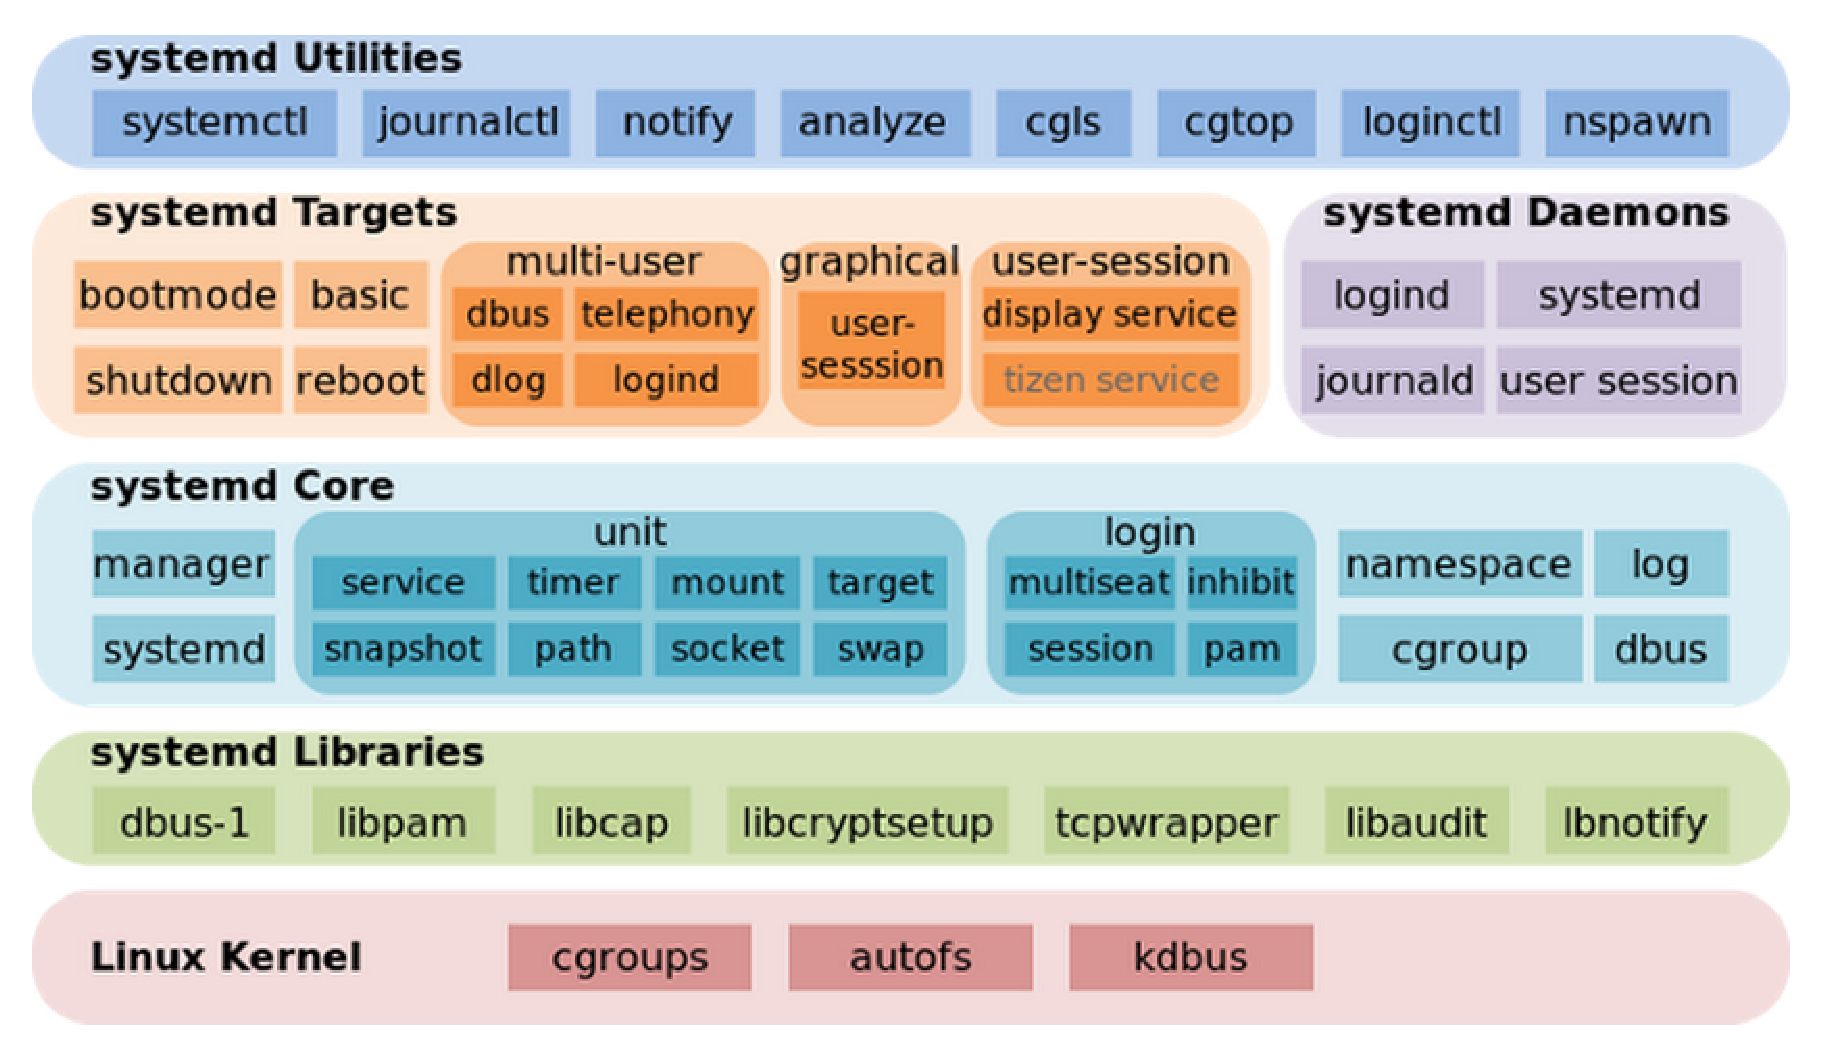
\includegraphics[height=5cm,
    angle=0]{./images/systemd.eps}}
  \caption{systemd architecture}
  \label{fig:systemd}
\end{figure}

\url{http://unix.stackexchange.com/questions/5877/what-are-the-pros-cons-of-upstart-and-systemd}

\subsection{-- concept: units}
\label{sec:systemd-unit-file}

In systemd, the target of most actions are "units", which are resources that
systemd knows how to manage. Units are categorized by the type of resource they
represent and they are defined with files known as unit files.  A unit file has
a suffix of \verb!.service!. 

NOTE: unit files are groupped together based on target (Sect.\ref{sec:targets}).

Start/stop a service (i.e. a unit file) using systemctl
(Sect.\ref{sec:systemctl}):
\begin{verbatim}
sudo systemctl start <application-name>.service
\end{verbatim}

List all units
\begin{verbatim}
   // all active units
sudo systemctl
sudo systemctl list-units

   //all of the units that systemd has loaded (or attempted to load), regardless
   // of whether they are currently active, 
sudo systemctl list-units --all
   // only 'active'-state units
sudo systemctl list-units --all --state=active

   // only 'service'-type units
sudo systemctl list-units --all --type=service


-------------------------------------------------------------------------------
UNIT                                      LOAD   ACTIVE SUB     DESCRIPTION
atd.service                               loaded active running ATD daemon
avahi-daemon.service                      loaded active running Avahi mDNS/DNS-SD Stack

LOAD = if the unit configuration file is parsed by systemd
ACTIVE = if the unit is loaded successfully?
SUB    =  lower-level state that indicates more detailed information about the
         unit  (running, exited)
DESCRIPTION = short textual description
\end{verbatim}



List unit files
\begin{verbatim}
systemctl list-unit-files

  // state will usually be "enabled", "disabled", "static", or "masked". I
  // static   = unit file has no 'install' section
  //             (as such, the unit can not be enabled)
  //            Usually, this means that the unit performs a one-off action or
  //            is used only as a dependency of another unit and should not be
  //            run by itself.
  
  
  
-----------------------------------------------------------------------
UNIT FILE                                  STATE   
proc-sys-fs-binfmt_misc.automount          static  
dev-hugepages.mount                        static  
\end{verbatim}

Display the file content of a unit file
\begin{verbatim}
  // old systemd support 'cat' 
systemctl cat atd.service
\end{verbatim}


Edit the file content of a unit file
\begin{verbatim}
  // /etc/systemd/system
sudo systemctl edit nginx.service
\end{verbatim}

\url{https://www.digitalocean.com/community/tutorials/how-to-use-systemctl-to-manage-systemd-services-and-units}

\subsection{-- concept: target}
\label{sec:systemd-target}

Targets are special unit files that describe a system state or synchronization
point (Sect.\ref{sec:systemd-unit-file}).
Like other units, the files that define targets can be identified by their
suffix, which in this case is .target.

Targets do not do much themselves, but are instead used to group other units
together.

\textcolor{red}{default target}:
\begin{verbatim}
>> systemctl get-default
  // /etc/systemd/system/default.target

graphical.target 
   // which is equivalent to runlevel 5 (i.e. full user access with 
   //       graphical display and networking

\end{verbatim}

\textcolor{red}{Display all targets}
\begin{verbatim}
ls -al /lib/systemd/system/runlevel*
\end{verbatim}

So, there are more \verb!target!s than the traditional runlevel.
\begin{verbatim}
  RedHat 6                          RedHat 7
Traditional runlevel      New target name     Symbolically linked to...
Runlevel 0           |    runlevel0.target -> poweroff.target
Runlevel 1           |    runlevel1.target -> rescue.target
Runlevel 2           |    runlevel2.target -> multi-user.target
Runlevel 3           |    runlevel3.target -> multi-user.target
Runlevel 4           |    runlevel4.target -> multi-user.target
Runlevel 5           |    runlevel5.target -> graphical.target
Runlevel 6           |    runlevel6.target -> reboot.target
\end{verbatim}  


\subsection{-- systemctl}
\label{sec:systemctl}

\verb!systemctl! command is the central management tool for controlling
the processed managed by \verb!systemd!, which is part of the the init system of
systemd (Sect.\ref{sec:systemd}). Before that, we use \verb!update-rc.d! command
(Sect.\ref{sec:update-rc.d}) or \verb!service! (Sect.\ref{sec:init-subsystem})
or \verb!initctl! (Sect.\ref{sec:Upstart}).

Not all distros has \verb!systemd! running as default
(Sect.\ref{sec:systemd-adoption}). Default package on Ubuntu 14.04 is
\verb!systemd-services! that doesn't provides the \verb!systemdctl! command. To
install on Ubuntu 14.04 (though some claims it does NOT work)
\begin{verbatim}
  // Step 1: backup 
sudo cp /etc/default/grub /etc/default/grub.bak

  // Step 2: edit the grub file /etc/default/grub
GRUB_CMDLINE_LINUX_DEFAULT = "init=/lib/systemd/systemd" 

// Step 3: install  
// https://launchpad.net/~pitti/+archive/ubuntu/systemd

sudo add-apt-repository ppa:pitti/systemd
sudo apt-get update
sudo apt-get dist-upgrade 

  // Step 4: 
sudo update-grub


// recover if needed
$ sudo mv /etc/default/grub.bak /etc/default/grub
$ sudo update-grub
\end{verbatim}
\url{http://linuxg.net/how-to-install-and-test-systemd-on-ubuntu-14-04-trusty-tahr-and-ubuntu-12-04-precise-pangolin/}

In Ubuntu 15.04 which has both, to switch from Upstart to
systemd, we can do (then reboot the machine)
\begin{verbatim}
apt-get install --reinstall systemd-sysv ubuntu-standard
\end{verbatim}
\url{https://wiki.ubuntu.com/SystemdForUpstartUsers}


Start/stop a service:
\begin{verbatim}
sudo systemctl start application.service

sudo systemctl start application

// [start | stop | restart | reload | reload-or-restart]
// [enable | disable]
// [status | is-active | is-enabled | is-failed]

 // reload = reload configuraiton file (without restarting)
\end{verbatim}

Example of a status of a service
{\tiny
\begin{verbatim}
 nginx.service - A high performance web server and a reverse proxy server
   Loaded: loaded (/usr/lib/systemd/system/nginx.service; enabled; vendor preset: disabled)
   Active: active (running) since Tue 2015-01-27 19:41:23 EST; 22h ago
 Main PID: 495 (nginx)
   CGroup: /system.slice/nginx.service
           |_495 nginx: master process /usr/bin/nginx -g pid /run/nginx.pid; error_log stderr;
           |_496 nginx: worker process
Jan 27 19:41:23 desktop systemd[1]: Starting A high performance web server and a reverse proxy server...
Jan 27 19:41:23 desktop systemd[1]: Started A high performance web server and a reverse proxy server.
\end{verbatim}
}





\section{File system}
\label{sec:file-system}

Linux supports at least 15 file systems; ext, ext2, xia, minix, umsdos, msdos,
vfat, proc, smb, ncp, iso9660, sysv, hpfs, affs and ufs.

When disks are initialized (using \verb!fdisk!, say) they have a partition
structure imposed on them that divides the physical disk into a number of
logical partitions. {\it Each partition may hold a single file system.}
A {\bf file system} is a way to organize data into files and directories.
A file system has to look, feel and operate in the same way no matter what
device is holding it. The file system might not even be on the local system, it
could just as well be a disk remotely mounted over a network link.

\begin{itemize}
  \item minix: filename cannot be longer than 14 characters, max file size 64MB
  
  This first file system that Linux had is rather restrictive and lacking in
  performance.
  
  \item ext (introduced 1992):
  

  
  \item ext2 (introduced 1993, by Rémy Card): no journaling feature (i.e. no
  overhead which is good on flash drives, usb drives), max file size 16GB to
  2TB, max filesystem size 2TB to 32TB.
  
  \item ext3 (introduced 2001, by Stephen Tweedie, since Linux 2.4.15):
  a directory can contain upto 32K subdirectories, 
  added journaling feature (to track all changes, i.e. less chance for
  corruption of filesystem) - 3 types of journaling
  \begin{itemize}
    \item Journal - Metadata and content are saved in the journal.

    \item Ordered - Only metadata is saved in the journal. Metadata are 
    journaled only after writing the content to disk. This is the default.
    
    \item Writeback - Only metadata is saved in the journal. Metadata might be 
    journaled either before or after the content is written to the disk.
  \end{itemize}
  
   \item ext4 (introduced 2008, sine Linux 2.6.19): max file size 16GB to 16 TB,
   max filesystem size 1 EB (exabyte) = $(10^{10})^{10}$TB, a directory can
   contain upto 64K subdirectories; journaling can be turned off; new features: 
   multiblock  allocation, delayed allocation, journal checksum. fast fsck, etc.
   
   \item btrfs (B-tree filesystem)
\end{itemize}


All file systems, of whatever type, are mounted onto a directory and the files
of the mounted file system cover up the existing contents of that directory.

Since ext, the real file systems were separated from the operating system and
system services by an interface layer known as the Virtual File system, or VFS
(Sect.\ref{sec:virtual-filesystem}). This separate the management of the
filesystem from the Linux kernel, i.e. all file systems appear identical to the
rest of the Linux kernel as the kernel talks to VFS; while VFS deals with
different underlying filesystems.

References:
\begin{itemize}
  \item \url{http://www.tldp.org/LDP/tlk/fs/filesystem.html}
\end{itemize}
  
% Regardless of which type, or how many, Linux treats single hierarchical tree
% structure that represents the file system as one whole single entity


\section{Virtual file-system (VFS)}
\label{sec:virtual-filesystem}


To help working with different filesystem (Sect.\ref{sec:file-system}), Linux
kernel move that management to the the virtual file-systems (VFS).
VFS describes the system's files in terms of superblocks and inodes in much the
same way as the EXT2 file system uses superblocks and inodes. 

As each file system is initialised, it registers itself with the VFS, and only
that time the real filesystem is loaded to manage the mounted disk. This enables
the Linux kernel to load the real filesystem only needed, rather than built into
the kernel code.
Example: VFAT file system is implemented as a kernel module, then it is only
loaded when a VFAT file system is mounted.


A Linux system has some virtual file-systems, each has its
specific purpose and daemons to perform the same functions.
\begin{enumerate}
  \item specfs (Sect.\ref{sec:specfs})
  \item devfs (which is replaced by \verb!udev! - Sect.\ref{sec:udev}) -
  Sect.\ref{sec:devfs}
  \item tmpfs - Sect.\ref{sec:tmpfs}
\end{enumerate}
   
\subsection{specfs}
\label{sec:specfs}

Special FileSystem (specfs) is a virtual filesystem used to access special
devices. This filesystem requires no mount-point, yet can be mounted by user
\begin{verbatim}
mount -t specfs none /dev/streams
\end{verbatim}
The device files for the character devices (Sect.\ref{sec:device_character}) use
specfs.

\subsection{devfs (Dev-FS)}
\label{sec:devfs}

\verb!devfs! is a device-manager (Dev-FS) in the form of a filesystem.
\verb!devfs! manages most other devices in /dev. 

To reduced the number of files in \verb!/dev! folder, Dev-FS was developed
\footnote{\url{http://sg.danny.cz/scsi/devfs_scsi.html}}. A replacement for
Dev-FS is \verb!udev! (Sect.\ref{sec:udev}).

Most Unix and Unix-like systems use \verb!devfs! (Mac OS X, *BSD, and Solaris)
on the kernel-space. Most Linux uses \verb!devfs! on a userspace - kernelspace
hybrid approach.

\verb!devfs! was added to Linux development source tree at kernel version
2.3.46, and was first introduced officialy into Linux kernel 2.4. It helps
reduced the number of files in \verb!/dev! folder to about

\begin{verbatim}
  // about 470
ls /dev | wc 

  // about 960  
du -a /dev | wc  
\end{verbatim}
\footnote{\url{http://sg.danny.cz/scsi/devfs_scsi.html}}

% In old Linux kernels (2.3.46pre5-2.6.17), the device
% folder is managed by Dev-FS (\verb!devfs!) and There is no way
% to identify hardware devices actually present in the system.



\subsection{devtmpfs}
\label{{sec:devtmpfs}}

\verb!devtmpfs! is designed to improve boot-time. 
It is where the devices information are stored, and the mount point is
\verb!/dev!.

\subsection{initrd  (INITial RamDisk): until Linux 2.5}
\label{sec:initrd}

\verb!initrd! refers to a file, e.g. initrd.img, that serves as an {\it initial
root filesystem} (RFS - Sect.\ref{sec:RFS}) (the filesystem is created by the
Linux kernel and only exist in RAM) that is loaded into memory prior to the real
root filesystem is available, i.e.
to bootstrap the O/S. This initial ramdisk is used to load drivers and
initialize an environment so that an external storage system (disk or network
attached storage) can be mounted.

initrd  acts as a block device (called \verb!ramdev!), so requires a filesystem
driver (e.g. ext2). It means the kernel must have at least one built-in module
for detecting filesystem. Also as it is a block device, it is cached, i.e. waste
memory and memory bus bandwidth.

\verb!initrd! (Initial RamDisk) is used until Linux kernel 2.5.
From Linux kernel 2.6, \verb!initrd! is deprecated, and is replaced by
\verb!initramfs! (Sect.\ref{sec:initramfs}). Limitation of initrd
\begin{enumerate}
  \item the image file has to be fixed size
  \item it requires at least one file system driver be compiled into the kernel,
  so that the image file (which is stored on a disk) can
  be read (from the disk with that file system)
  
  \item all of the reads/writes on Initrd are buffered redundantly
  (unnecessarily) into main memory
\end{enumerate}



\subsection{-- create initrd (*.img image file)}
\label{sec:initrd-create-it}

An initrd image file is a block device (Sect.\ref{sec:block-device}). This means
the contents of the file have to be formatted and prepared with special tools
(such as \verb!mke2fs! and \verb!losetup!), and like all block devices it
requires a filesystem driver to interpret the data at runtime (see below on how
to create such file).

% The reason to use this is that the kernel can use this filesystem to load the
% kernel module that can make the real root filesystem.

Depending on which version of Linux you're running, the method for creating the
initial RAM disk can vary.
\begin{itemize}
  \item OPTION 1: manually build a custom initial RAM disk using \verb!mke2fs!,
  and \verb!Losetup!i.e.   write the script as give below \verb!mkird! and run
  each time you want to create an initial RAM disk
  
  \item OPTION 2: create a complete RFS folder structure (Sect.\ref{sec:RFS}), 
  and then run \verb!genext2fs! utility
%   \item  When you compile a kernel, and build a kernel image, you'll get a
%   matching \verb!initrd! file automatically.

  \item OPTION 3: \verb!mkinitrd! tool, but only build the initrd for the
  current machine.
  
  This command is often used to rebuild the initrd of the current machine; not
  for a different machine.
  
  \item OPTION 4: \verb!YAIRD! (Yet Another Mkinitrd) utility, which permits
  customization of every aspect of the initrd construction.
  
\end{itemize}

\textcolor{red}{OPTION 1a: require root}: save the following code as
\verb!mkird! script, which can be used to create an initial RAM disk. You need to be at
'root', and performing all necessary folders, files, devices creation.

\textcolor{red}{This code create a file as a loopback device}: explains
\begin{itemize}
  \item  To create an initrd, begin by creating an empty file, using /dev/zero
  (a stream of zeroes) as input writing to the ramdisk.img file.
  
  The size is fixed and has to be  4MB in size (4000 1K blocks).
  \begin{verbatim}
  RDSIZE=4000
  BLKSIZE=1024
  \end{verbatim}
  
  \item Make the image file as ext2 filesystem
  \begin{verbatim}
  /sbin/mke2fs
  \end{verbatim}
  
  \item Mount the image to \verb!/mnt/initrd! using a loop device, so that we
  can create the directory structures and put utilities on it.
  
  We can use Busybox for the set of essential utilities
  (Sect.\ref{sec:busybox}) and
  make sure it is compiled for
  the right target machine where
  the kernel runs (Sect.\ref{sec:busybox-compile-target-machine})
  
  \item While mounting, also create a set of special devices inside \verb!/dev!
  folder.
  
  \item and create \verb!/initrd/linuxrc! file (the file to be run once the
  initrd is still being used as the initial root filesystem): whose goal is to
  mount the real root filesystem.
  
%   After the kernel mount the RAM disk, it searches for the first user-space
%   program to execute, which is an \verb!init! file to execute
%   (Sect.\ref{sec:init}). If an init file is not found, the kernel invokes the
%   linuxrc file as its startup script.
  
  \item Finally, unmount it, and then we compress into gzip (e.g.
  rmadisk.img.gz) for further use.
\end{itemize}

{\footnotesize 
\begin{verbatim}
#!/bin/bash

# Housekeeping...
rm -f /tmp/ramdisk.img
rm -f /tmp/ramdisk.img.gz

# Ramdisk Constants, i.e. we create 4MiB RAM disk
# 4000 blocks, each block 1024bytes
RDSIZE=4000
BLKSIZE=1024

# Create an empty ramdisk image
dd if=/dev/zero of=/tmp/ramdisk.img bs=$BLKSIZE count=$RDSIZE

## OPTION 1a:
# Make it an ext2 mountable file system
/sbin/mke2fs -F -m 0 -b $BLKSIZE /tmp/ramdisk.img $RDSIZE

# Mount it so that we can populate
mkdir /mnt/initrd -p
mount /tmp/ramdisk.img /mnt/initrd -t ext2 -o loop=/dev/loop0

## END OPTION 1a
## OPTION 1b
# NOTE:
#    We can also associate the image file with a loopback device 
#losetup /dev/loop0 /tmp/ramdisk.img
#mke2fs /dev/loop0
#mount /dev/loop0 /mnt/initrd
## END OPTION 1b

# Populate the filesystem (subdirectories)
# NOTE:
#   if we already have a RFS in my_rfs/
#   then we just 'cp -a my_rfs/ /mnt/initrd
#   and then do not need the following
mkdir /mnt/initrd/bin
mkdir /mnt/initrd/sys
mkdir /mnt/initrd/dev
mkdir /mnt/initrd/proc

# Grab busybox and create the symbolic links
pushd /mnt/initrd/bin
cp /usr/local/src/busybox-1.1.1/busybox .
ln -s busybox ash
ln -s busybox mount
ln -s busybox echo
ln -s busybox ls
ln -s busybox cat
ln -s busybox ps
ln -s busybox dmesg
ln -s busybox sysctl
popd

# Grab the necessary dev files
cp -a /dev/console /mnt/initrd/dev
cp -a /dev/ramdisk /mnt/initrd/dev
cp -a /dev/ram0 /mnt/initrd/dev
cp -a /dev/null /mnt/initrd/dev
cp -a /dev/tty1 /mnt/initrd/dev
cp -a /dev/tty2 /mnt/initrd/dev

# Equate sbin with bin
pushd /mnt/initrd
ln -s bin sbin
popd

# Create the init file
cat >> /mnt/initrd/linuxrc << EOF
#!/bin/ash
echo
echo "Simple initrd is active"
echo
mount -t proc /proc /proc
mount -t sysfs none /sys
/bin/ash --login
EOF

chmod +x /mnt/initrd/linuxrc

# Finish up...
umount /mnt/initrd

# Compress the image
# -9 = the slowest 
gzip -9 /tmp/ramdisk.img
# or if you want a custome file name
#  gzip -9 -c /tmp/ramdisk.img > /tmp/filename.gz 
cp /tmp/ramdisk.img.gz /boot/ramdisk.img.gz
\end{verbatim}}
\url{http://www.ibm.com/developerworks/library/l-initrd/}


\textcolor{red}{OPTION 2: without root}:
The method described in OPTION 1 requires root permission to mount an empty
image. To avoid this, we discuss a method that uses \verb!genext2fs! and
\verb!fakeroot!. However, we still needs root right to install the two utilities
first
\begin{verbatim}
sudo apt-get install genext2fs fakeroot
\end{verbatim}

Now, without root, suppose you want to create \verb!ext2! filesystem image using
\verb!genext2fs! tool
\begin{enumerate}
  \item first make sure you have the proper folder structure for a RFS
  (Sect.\ref{sec:RFS})

Example: in folder \verb!initrd/! to make an initrd.
\begin{verbatim}
drwxr-xr-x    7 root     root         1024 Sep 14 20:12 initrd/
drwxr-xr-x    2 root     root         1024 Sep 14 20:12 initrd/bin/
-rwxr-xr-x    1 root     root       436328 Sep 14 20:12 initrd/bin/insmod
-rwxr-xr-x    1 root     root       424680 Sep 14 20:12 initrd/bin/sash
drwxr-xr-x    2 root     root         1024 Sep 14 20:12 initrd/dev/
crw-r--r--    1 root     root       5,   1 Sep 14 20:12 initrd/dev/console
crw-r--r--    1 root     root       1,   3 Sep 14 20:12 initrd/dev/null
brw-r--r--    1 root     root       1,   1 Sep 14 20:12 initrd/dev/ram
crw-r--r--    1 root     root       4,   0 Sep 14 20:12 initrd/dev/systty
crw-r--r--    1 root     root       4,   1 Sep 14 20:12 initrd/dev/tty1
crw-r--r--    1 root     root       4,   1 Sep 14 20:12 initrd/dev/tty2
crw-r--r--    1 root     root       4,   1 Sep 14 20:12 initrd/dev/tty3
crw-r--r--    1 root     root       4,   1 Sep 14 20:12 initrd/dev/tty4
drwxr-xr-x    2 root     root         1024 Sep 14 20:12 initrd/etc/
drwxr-xr-x    2 root     root         1024 Sep 14 20:12 initrd/lib/
-rwxr-xr-x    1 root     root           76 Sep 14 20:12 initrd/linuxrc
drwxr-xr-x    2 root     root         1024 Sep 14 20:12 initrd/loopfs/
\end{verbatim}
and the content of \verb!initrd/linuxrc! file should load all the modules needed
for the kernel to access the SCSI partition, for example.
\begin{verbatim}
#!/bin/sash
 
aliasall
 
echo "Loading aic7xxx module"
insmod /lib/aic7xxx.o 
\end{verbatim}

\begin{verbatim}
chroot ~/initrd /bin/sash
/linuxrc
\end{verbatim}

  
  \item suppose the folder that contains the proper RFS structure is named
  \verb!rootfs!; then we issues these commands

Example: create 8MB sized ext2 image called initrd.img with the content of the
directory rootfs (8MB = 1024x8 = 8192)
\begin{verbatim}
genext2fs -d rootfs -b 8192 initrd.img

  # add '-U' for making all files owned by root 
  # (i.e. root squashing feature)
  # DO NOT use this if the content already have
  #    the correct ownership
genext2fs -d rootfs -b 8192 -U initrd.img
\end{verbatim}
and then compress
\begin{verbatim}
gzip -9 < initrd.img > initrd.bin
\end{verbatim}
we can use the final compressed image \verb!initrd.bin! to flash to the embedded
device.
  
Example: 
\begin{verbatim}
$ ROOTFS_DIR=rootfs                 # directory with root file system content
$ ROOTFS_SIZE=3700                  # size of file system image
$ ROOTFS_FREE=100                   # free space wanted
$ ROOTFS_INODES=380                 # number of inodes
$ ROOTFS_DEVICES=rootfs_devices.tab # device description file
$ ROOTFS_IMAGE=ramdisk.img          # generated file system image

$ genext2fs -U \
        -d ${ROOTFS_DIR} \
        -D ${ROOTFS_DEVICES} \
        -b ${ROOTFS_SIZE} \
        -r ${ROOTFS_FREE} \
        -i ${ROOTFS_INODES} \
        ${ROOTFS_IMAGE}
\end{verbatim}


Finally compress the image with gzip
\begin{verbatim}
$ gzip -v9 ramdisk.img
rootfs.img:      55.6% -- replaced with ramdisk.img.gz
\end{verbatim}
\begin{verbatim}
dd if=ramdisk.img bs=1k | gzip -v9 > rootfs.gz
\end{verbatim}


\end{enumerate}

\textcolor{red}{OPTION 3}: \verb!mkinitrd!  utility
can be used to create an initrd file for the current machine (not for a
different machine) using the kernel modules in  \verb!/lib/modules/! folder
\begin{verbatim}
/sbin/mkinitrd --help   # Or simply type 'mkinitrd --help'
usage: mkinitrd [--version] [-v] [-f] [--preload <module>]
       [--omit-scsi-modules] [--omit-raid-modules] [--omit-lvm-modules]
       [--with=<module>] [--image-version] [--fstab=<fstab>] [--nocompress]
       [--builtin=<module>] [--nopivot] <initrd-image> <kernel-version>
  
   -v = verbose (display all modules being included in the initrd)
   -f = force (overwrite any existing initrd image)
       (example: mkinitrd /boot/initrd-2.2.5-15.img 2.2.5-15)
       
  # create initrd file for the current kernel
  # (make sure to backup first)
cp /boot/initrd-$(uname -r).img /boot/initrd-$(uname -r).img.bak  
mkinitrd -f -v /boot/initrd-$(uname -r).img $(uname -r)  
         
  # create the file /boot/initrd-2.4.20-8.img
  # for a particular kernel version, e.g. 2.4.20-8
   
mkinitrd /boot/initrd-2.4.20-8.img 2.4.20-8

  # (default) create /boot/initrd file
  #  -k <kernel-version>
  #  -m [reiserfs | ext3 | ext2 ]   
  #     
mkinitrd -c -k 2.6.37.6 -m reiserfs

  # make the initrd to run on Xen hypervisor
mkinitrd --with-xenblk initrd-2.6.18-371.el5xen.img 2.6.18-371.el5xen  
\end{verbatim}
NOTE: Check the patch below for \verb!mkinitrd!
\url{https://bugs.debian.org/cgi-bin/bugreport.cgi?bug=212602}


In desktop and server Linux, the \verb!initrd! lifetime is short, only serving
as a bridge to the real root file system. It mounts the real root filesystem
onto a temporary mount point on the initrd, then invokes \verb!pivot_root(8)! to
swap the root and temporary mount points, leaving the initrd in a position to be
umounted and the actual root filesystem on /.

In embedded systems with no mutable storage, the initrd is the permanent root
file system. Because there is no hard drive in many embedded systems based on
Linux, the initrd also serves as the permanent root file system.

  

Nowadays, \verb!initrd! are files in cpio-format, and can be inspected using
\begin{verbatim}
# gunzip -c /boot/initrd-2.6.31.img > /tmp/my_initrd
 $ cpio -it < /tmp/my_initrd         [examine contents]
 lib
 lib/udev
 lib/udev/console_init
 lib/firmware
 lib/firmware/radeon
 lib/firmware/radeon/RV730_me.bin
 ... snip ...
 lib/modules
 lib/modules/2.6.31
 lib/modules/2.6.31/radeon.ko
 lib/modules/2.6.31/modules.isapnpmap
 ... and so on and so on ...
 $ cd [somewhere]                    [in preparation for unloading]
 $ cpio -i < /tmp/my_initrd          [unload] 
\end{verbatim}

Example: 
\begin{verbatim}
drwxr-xr-x  10 root root    4096 May 7 02:48 .
drwxr-x---  15 root root    4096 May 7 00:54 ..
drwxr-xr-x  2  root root    4096 May 7 02:48 bin
drwxr-xr-x  2  root root    4096 May 7 02:48 dev
drwxr-xr-x  4  root root    4096 May 7 02:48 etc
-rwxr-xr-x  1  root root     812 May 7 02:48 init
-rw-r--r--  1  root root 1723392 May 7 02:45 initrd-2.6.14.2.img
drwxr-xr-x  2  root root    4096 May 7 02:48 lib
drwxr-xr-x  2  root root    4096 May 7 02:48 loopfs
drwxr-xr-x  2  root root    4096 May 7 02:48 proc
lrwxrwxrwx  1  root root       3 May 7 02:48 sbin -> bin
drwxr-xr-x  2  root root    4096 May 7 02:48 sys
drwxr-xr-x  2  root root    4096 May 7 02:48 sysroot
\end{verbatim}
The \verb!init! file, like the traditional Linux boot process, is invoked when
the initrd image is decompressed into the RAM disk. 

% There are two implementation of \verb!initrd!
% \begin{itemize}
%   \item old \verb!initrd! (ramdisk) :  
%   
%   \item new \verb!initrd! (\verb!ramfs! and \verb!tmpfs!): 
%   %  unpacked via \verb!cpio! into the memory
% \end{itemize}
% \url{http://stackoverflow.com/questions/10603104/the-difference-between-initrd-and-initramfs}

\subsection{initramfs (cpio-archive file-based)}
\label{sec:initramfs}

INITial RAM FileSystem (initramfs) was added to Linux kernel from 2.6, and is
the better replacement for \verb!initrd! (Sect.\ref{sec:initrd}).
Initramfs is an instance of \verb!tmpfs!, i.e. RAM-based filesystems that
automatically grow or shrink to fit the size of the data they contain.

\begin{mdframed}
As RAM is still faster than even modern SSD (solid-state driver), RAM disks take
advantage of this, using your computer's RAM as a lightning-fast virtual drive.
First you need to create an image file containg everything needed for a Linux
root filesystem (RFS) and the Linux kernel.
This file is a compressed filesystem image file, containing a minimal set of
directories and executables to achieve this, such as the \verb!insmod! tool to
install kernel modules into the kernel.
Once the machine boot-up, a boot loader (e.g. U-boot) reads the content of this
image file, and loads them into the RAM, reserving this area of RAM as the
physical disk.
\end{mdframed}

While \verb!initrd! is block-device based (which is mountable - look how an
initrd image is created), \verb!initramfs! is file-based (which is
cpio-archive).

\begin{itemize}
  \item With initrd, you created a file system image. 
  
  \item With initramfs, you create an archive with the files.

There's no duplication between block device and cache, because there's no block
device. A system using initramfs as its root filesystem doesn't even need a
single filesystem driver built into the kernel, because there are no block
devices to interpret as filesystems.
\end{itemize}
\url{http://landley.net/writing/rootfs-intro.html}

Once \verb!tmpfs! is mounted as the root, the \verb!initramfs! cpio-archive file
is extracted to tmpfs (Sect.\ref{sec:tmpfs}).
To load the real root filesystem, the initramfs boot scripts mount the real root
in \verb!/root!, delete all files in the tmpfs root, then chroot into /root, and
exec the file /sbin/init inside initramfs.

\subsection{-- create initramfs}
\label{sec:initramfs-create-option-1}
  
\textcolor{red}{\bf OPTION 1 - create a custom initramfs}: To create an
initramfs cpio-archive file, we follow (1) create some folders, (2) put
some utilities (e.g. Busybox compiled for the target machine -
Sect.\ref{sec:busybox-compile-target-machine}), (3) the top folder needs to
contain a program called \verb!init!

\begin{verbatim}
mkdir initramfs
cd initramfs/
mkdir -pv bin lib dev etc mnt/root proc root sbin sys
sudo cp -va /dev/{null,console,tty} dev/

  # copy freshly-buit Busybox
sudo cp -avR <busybox>/_install/* ../initramfs/
\end{verbatim}
check what libraries is needed for Busybox 
\begin{verbatim}
ldd bin/busybox
        linux-gate.so.1 =>  (0xf76f7000)
        libm.so.6 => /usr/lib/libm.so.6 (0xf76a1000)
        libc.so.6 => /usr/lib/libc.so.6 (0xf74fe000)
        /lib/ld-linux.so.2 (0xf76f8000)
\end{verbatim}
and then copy them to
\verb!initramfs/usr/lib!
\begin{verbatim}
mkdir -pv usr/lib
# copy the right libraries above 
#      to the right location (/usr/lib, /lib)
# e.g.
#cp -av /usr/lib/lib[mc].so.6 usr/lib/
#cp -av /usr/lib/lib[mc]-2.16.so usr/lib/
#cp -av /usr/lib/ld-2.16.so usr/lib/
#cp -av /lib/ld-linux.so.2 lib/
#cp -av /lib/ld-2.16.so lib/
\end{verbatim}

Next step, create the \verb!initramfs/init!. There are different ways to do this
\begin{itemize}
  \item simply use the Busybox which provide \verb!init!-like feature
  
\begin{verbatim}
ln -s /bin/busybox /init
\end{verbatim}

  \item create your own \verb!init! script
  
\begin{verbatim}
emacs initramfs/init
\end{verbatim}
and put the content
\begin{verbatim}
#!/bin/sh

/bin/mount -t proc none /proc
/bin/mount -t sysfs sysfs /sys

cat <<'EOF'
                       _             _ _                  
 _ __ ___   __ _  __ _| | __ _ ___  | (_)_ __  _   ___  __
| '_ ` _ \ / _` |/ _` | |/ _` / __| | | | '_ \| | | \ \/ /
| | | | | | (_| | (_| | | (_| \__ \ | | | | | | |_| |>  < 
|_| |_| |_|\__, |\__,_|_|\__, |___/ |_|_|_| |_|\__,_/_/\_\
           |___/         |___/                            

EOF
echo 'Enjoy your new system!'

/bin/sh
\end{verbatim}
\end{itemize}
and make it executable
\begin{verbatim}
chmod 755 ~/linux_qemu/initramfs/init
\end{verbatim}

Final step, create the cpio archive from the folder
\begin{verbatim}
cd initramfs
find . -print0 | cpio --null -ov --format=newc > ../my-initramfs.cpio
\end{verbatim}
We avoid gzip'ing it here because the emulator takes forever to unpack it if we
do.
\url{http://mgalgs.github.io/2012/03/23/how-to-build-a-custom-linux-kernel-for-qemu.html}

\textcolor{red}{Incorporate the initramfs into the Linux kernel image}:
(Sect.\ref{sec:build_Linux-kernel-with-initramfs}).

The easiest way to use initramfs is to replace the kernel's built-in empty cpio
archive with a non-empty one. Just before recompile the kernel, we enable the
kernel config option
\begin{verbatim}
make menuconfig
   CONFIG_INITRAMFS_SOURCE=</point/to/localtion/of/initramfs/file>
\end{verbatim} 

\subsection{-- create initramfs}
\label{sec:initramfs-create-option-2}

\textcolor{red}{\bf OPTION 2 - rebuild the initramfs of the current machine}:
 
Different Linux distributions use different initramfs frameworks like e.g.
\verb!dracut! for Fedora, RHEL6+; or \verb!initramfs-tools! for Debian.

\begin{verbatim}
# First backup the initramfs
cp /boot/initramfs-$(uname -r).img /boot/initramfs-$(uname -r).img.bak
  # rebuild the initramfs for the current kernel
dracut -f
  # rebuild ... for a specific kernel version, e.g. 2.6.32-71.el6.x86_64
dracut -f initramfs-2.6.32-71.el6.x86_64.img 2.6.32-71.el6.x86_64
\end{verbatim}

Most common solutions are either using something like \verb!udev!, \verb!mdev!
or \verb!devtmpfs! (Sect.\ref{sec:devtmpfs}).
Some may also just use MAKEDEV to generate a static layout or have the device
files already integrated into their image.

If you boot without an initramfs the kernel can just boot from devices with
known major/minor numbers, e.g. /dev/sda1 but not from lvm devices.

\url{http://askubuntu.com/questions/14961/what-is-the-difference-between-initrd-and-initramfs}
%It is a common filesystem that is used on memory

\url{https://www.linux.com/learn/linux-training/92607-the-kernel-newbie-corner-qinitrdq-and-qinitramfsq-whats-up-with-that}

\url{http://stackoverflow.com/questions/10603104/the-difference-between-initrd-and-initramfs}

\subsection{ramdisk}
\label{sec:ramdisk}
\label{sec:RAMDISK-for-RFS}


In Linux it is also possible to have another type of virtual device mounted as a
filesystem, this is the ramdisk device. A ramdisk is a set of blocks that gets
copied to an allocated chunk of memory, then treated as a block device. A normal
filesystem is created on the ramdisk.

Like initrd (Sect.\ref{sec:initrd}), ramdisk is a RAM-based block device, i.e.
a file with fixed size chunk of memory that can be mounted like a disk.
% A ramdisk refers to a disk-like device located on RAM.
The downside of the ramdisk pretending to be a block device is it gets treated
like a block device. 

In this case the device does not refer to any physical hardware, but to a
portion of memory that is set aside for the purpose. The memory that is
allocated is never swapped out to disk, but remains in the disk cache.
So, ramdisk even waste more memory than initrd due to caching.

As Linux is designed to cache all files and directory entries read from or
written to block devices, so Linux copies data to and from the ramdisk into the
"page cache" (for file data), and the "dentry cache" (for directory entries).

Creating a RAMDISK image is the same as creating an initrd, so just follows the
example given (Sect.\ref{sec:initrd}). A ramdisk can be created at any time by
writing to the ramdisk device at \verb!/dev/ram0! or \verb!/dev/ram1! etc. This
can then be formatted and mounted in the same way that the loopback device
(Sect.\ref{sec:loopback-device}) is.


\subsection{RAM (memory)-based filesystem: ramfs and tmpfs}


\verb!ramfs! and \verb!tmpfs! are two RAM-based storage filesystem that are
available to most modern Linux O/S.

As RAM is a volatile type of memory storage, the data is lost at system
restarted or turned off. 

The major benefit is that the data access is very fast, e.g. 10x faster than
modern SSDs.

\verb!ramfs! is older, and is largely replaced by \verb!tmpfs!.

RAMFS:
\begin{itemize}
  \item data stored is NOT removed when the memory exceeds threshold set by the system
  
  \item the size of the ramfs filesystem is NOT limited by the RAM installed. It continue using memory storage
  if it exceeds the size of RAM. Thus, we cannot see the size of this filesystem in \verb!df! tool, and can 
  only be estimated at the \verb!cached! entry in \verb!free! command.
\end{itemize}

TMPFS:
\begin{itemize}
  \item user set the size limit of the given tmpfs filesystem
  
  So, a diskfull error is returned when the limit is reached. The same behavior of a partition of a physical disk.
  Size is given from \verb!df! command.
  
  \item can use SWAP space if the system run out of RAM.
  
  SWAP space is indeed disk memory region.
\end{itemize}

\subsection{ramfs}
\label{sec:ramfs}


To replace ramdisk (Sect.\ref{sec:ramdisk}), Linus Torvalds suggested what if
Linux's cache could be stored on RAM, rather than disk cache and is mounted like
a filesystem.


Linus wrote a tiny wrapper around the cache called {\bf "ramfs"}, and other
kernel developers created an improved version called {\bf "tmpfs"} (which can
write the data to swap space, and limit the size of a given mount point so it
avoids to consuming all available memory) - Sect.\ref{sec:tmpfs}).

There's no duplication between block device and cache, because there's no block
device. The copy in the cache is the only copy of the data. Best of all, this
isn't new code but a new application for the existing Linux caching code, which
means it adds almost no size, is very simple, and is based on extremely well
tested infrastructure.

\url{http://landley.net/writing/rootfs-intro.html}

  
%   use a dummy
%   filesystem (called \verb!tmpfs!) and there is no extra copy of data in memory.
  

\subsection{tmpfs}
\label{sec:tmpfs}

\verb!ramfs!  (Sect.\ref{sec:ramfs}) is to replace ramdisk
(Sect.\ref{sec:ramdisk}). The downside of \verb!ramfs! is it does not prevent
memory fill-up. Check also \verb!rootfs! (Sect.\ref{sec:rootfs}).

\verb!tmpfs! is a derivative of ramfs, with adding size limits, and the ability
to write data to SWAP space if RAM memory capacity is reached. 


NOTE: The tmpfs image is a compressed \verb!cpio! file and is compressed into
the \verb!/tmpfs!
\begin{verbatim}
zcat initramfs | cpio -i
\end{verbatim}
\url{https://www.kernel.org/doc/Documentation/filesystems/ramfs-rootfs-initramfs.txt}


\begin{verbatim}

mkdir /mnt/ramdisk

mount -t tmpfs -o size=512m tmpfs /mnt/ramdisk


mount -t [TYPE] -o size=[SIZE] [FSTYPE] [MOUNTPOINT]

TYPE = ramfs, or tmpfs
SIZE  = 512m or 1024g (unit is 'm' = MB, 'g'=GB) 
		NOTE: if TYPE=ramfs, this number is used as the starting size
FSTYPE = tmpfs, ramfs, or ext4, ...
\end{verbatim}

To make the ramdisk persist over reboot, edit \verb!/etc/fstab/! file 
\begin{verbatim}
tmpfs    /mnt/ramdisk   tmpfs    nodev,nosuid,noexec,nodiratime,size=1024M   0   0
\end{verbatim}


\subsection{cramfs (embedded Linux)}
\label{sec:cramfs}

Embedded Linux systems need to use \verb!cramfs! (compressed RAM/ROM
filesystem), rather than \verb!initrd! (Sect.\ref{sec:initrd}) or other
filesystems to bootstrap the O/S. 

This is a read-only filesystem (which cannot be changed until the next creation
time at boot-time). The size of the filesystem is limited to 272 MB, and each
file not exceeds 16MB. Each page in the memory is compressed using zlib, but the
metadata is not in such a way to save memory without compression.

\subsection{SquashFS (embedded Linux)}
\label{sec:SquashFS}

This is an alternative to \verb!cramfs!, and is also a read-only filesystem. 
There is no limit if size of file or rootfs

SquashFS is often used in live-CD boot from Ubuntu, Arch or Fedora CD.

\subsection{UnionFS (overlay different filesystem)}
\label{sec:unionfs}

Suppose you have a music folder on your USB, and you want once you plug your USB
in your machine, you should have all the music combined of those in USB and
those in \verb!$HOME/Music! folder.

An overlay mount would allow a user to 'merge' the underlying tree (the Music
directory on the USB drive) with an "upper" one, \verb!$HOME/Music! on the
laptop, completely seamlessly.

Here, the multiple filesystems - one for USB storage, and one for local
harddrive (Sect.\ref{sec:file-system} - each is treated as a branch),
e.g. disks or partitions mounted from local or remote machines. The different
branches may be either read-only and read-write file systems.

These branches can be merged into a single view using UnionFS.
\textcolor{red}{LIMITATION: UnionFS requires the branches must come from
different filesystems}. Contents of directories which have the same path within
the merged branches will be seen together in a single merged directory, within
the new, virtual filesystem.

The different branches may be either read-only and read-write file systems.
Other options:
\begin{enumerate}
  \item mhddfs - Sect.\ref{sec:mhddfs}
  
  \item AuFS - Sect.\ref{sec:aufs}
  
  \item OverlayFS - Sect.\ref{sec:OverlayFS}
\end{enumerate}


\subsection{aufs (overlay diffferent filesystem)}
\label{sec:aufs}

AuFS (Another-Union-FS) is based on UnionFS (Sect.\ref{sec:unionfs}) developped
since 2006 by Junjiro Okajama.
AuFS is a re-design and re-implementation of UnionFS, with advanced
multi-layered unification filesystem. After adding many new original ideas it
became entirely separate from UnionFS (NOTE: some are being implemented in
UnionFS 2.x).
\begin{itemize}
  \item   writable branch balancing
  
  \item 
\end{itemize}

Current: 

It is being used as live-distro in Slax and Knoppis CD.


NOTE: AuFS was criticized for being "dense, unreadable, and uncommented"; and
OverlayFS was added into the kernel instead (Sect.\ref{sec:OverlayFS}).


\subsection{OverlayFS (overlay the same or different filesystems)}
\label{sec:OverlayFS}

Unlike some other overlay filesystems, the directory subtrees being merged by
OverlayFS do not necessarily have to be from distinct filesystems
\begin{itemize}
  \item   merging of directory access when both filesystems present a directory
  for the same name. 
  
NOTE: the directory subtrees being merged by OverlayFS do not necessarily have
to be from distinct filesystems
  
  \item Otherwise, OverlayFS presents the object, if any, yielded by one or the
  other, with the "upper" filesystem taking precedence.
  
  \item supports whiteouts and opaque directories in the upper filesystem to
  allow file and directory deletion
\end{itemize}

To create an overlay mount can be done purely with directories if desired as
demonstrated here

\begin{verbatim}
cd /tmp
mkdir lower upper workdir overlay
sudo mount -t overlay -o \
lowerdir=/tmp/lower,\
upperdir=/tmp/upper,\
workdir=/tmp/workdir \
none /tmp/overlay
\end{verbatim}
We can throw in a [virtual] block devices with their own filesystems (of any
kind) to act as the \verb!lower! and \verb!upper! filesystems if we desire. 
The only restriction is that the "workdir" needs to be an empty directory within
the same filesystem as the upperdir. An example using a filesystem for both the
upperdir and lowerdir can be shown below

{\tiny
\begin{verbatim}
cd /tmp

# Create the necessary directories.
mkdir lower upper overlay

# Lets create a fake block device to hold our "lower" filesystem
dd if=/dev/zero of=lower-fs.img bs=4096 count=102400
dd if=/dev/zero of=upper-fs.img bs=4096 count=102400

# Give this block device an ext4 filesystem.
mkfs -t ext4 lower-fs.img
mkfs -t ext4 upper-fs.img

# Mount the filesystem we just created and give it a file
sudo mount lower-fs.img /tmp/lower
sudo chown $USER:$USER /tmp/lower
echo "hello world" >> /tmp/lower/lower-file.txt

# Remount the lower filesystem as read only just for giggles
sudo mount -o remount,ro lower-fs.img /tmp/lower

# Mount the upper filesystem
sudo mount upper-fs.img /tmp/upper
sudo chown $USER:$USER /tmp/upper

# Create the workdir in the upper filesystem and the 
# directory in the upper filesystem that will act as the upper
# directory (they both have to be in the same filesystem)
mkdir /tmp/upper/upper
mkdir /tmp/upper/workdir

# Create our overlayfs mount
sudo mount -t overlay -o \
lowerdir=/tmp/lower,\
upperdir=/tmp/upper/upper,\
workdir=/tmp/upper/workdir \
none /tmp/overlay
\end{verbatim}
}

From kernel 4.0+
\begin{verbatim}
sudo mount -t overlay -o \
lowerdir=/tmp/lower:/tmp/lowest,\
upperdir=/tmp/upper,\
workdir=/tmp/workdir \
none /tmp/overlay
\end{verbatim}

Support for  Ubuntu 14.04 with the 3.19 kernel which should have OpenFS
supported (since kernel 3.18).


\subsection{mhddfs (overlay different filesystem)}
\label{sec:mhddfs}


\url{https://romanrm.net/mhddfs}

\begin{verbatim}
Server Name  Dir    Space
Server 1     /home  10 GB Space
Server 2     /home  10 GB Space
Server 3     /home  10 GB Space
\end{verbatim}
Using NFS (Sect.\ref{sec:NFS})
\begin{verbatim}
Server 1 /home to Server 3 /home/mount1
Server 2 /home to Server 3 /home/mount3
\end{verbatim}
On server 3, run mhddfs:
\begin{verbatim}
mhddfs /home/server/mount1,/home/server/mount2 /home/server/mount
\end{verbatim}

You can read from the virtual mount folder, i.e. /home/server/mount.

If you create and write to a new file in the virtual mount folder, it will be
put into the first branch, with enough free storage, i.e. the file cannot be
splitted across branches.

\subsection{rootfs}
\label{sec:rootfs}

A rootfs is not actually a separate or special filesystem; it refers to the root
of your system which may use any filesystem you choose.
Sect.\ref{sec:root-file-system} discusses how to create a working root file
system.


Rootfs is a special instance of ramfs (or tmpfs, if that's enabled -
Sect.\ref{sec:tmpfs}), which is always present in Linux 2.6 systems.
If \verb!tmpfs! is enabled it will be used by default. 
It's a fully capable ram based filesystem. So, you can use initramfs
(Sect.\ref{sec:initramfs}) as the rootfs. To force ramfs, add
"rootfstype=ramfs" to the kernel command line.


NOTE: If \verb!CONFIG_TMPFS! is enabled, then \verb!rootfs! uses \verb!tmpfs!
instead of \verb!ramfs! by default. In such case, to force using ramfs, add
\verb!rootfstype=ramfs! to the kernel command-line.

% The temporary filesystem (tmpfs) is a virtual FS for storing temporary files -
% an improvement of ramfs (Sect.\ref{sec:ramfs}).
The files are actually in the RAM memory or swap space. The mount point is /tmp,
and the content of the files are automatically lost after power shutdown or
system restart.

To enable \verb!tmpfs!, we compile the Linux kernel with
\begin{verbatim}
CONFIG_TMPFS
\end{verbatim}
then rootfs (Sect.\ref{sec:rootfs}) will use tmpfs instead of ramfs by
default.  


When a Linux kernel 2.6 boots, it mounts "rootfs" as its first filesystem.
This is a special instance of tmpfs which can't be moved or unmounted.
Most 2.6 systems just leave it empty and mount another root filesystem on top of
it, but rootfs is always there (check /proc/mounts to see) 
Only if the kernel can't run "/init" in rootfs will it fall back to the legacy
behavior of parsing the "root=" kernel command line to find another filesystem
to mount.
 

Potential booting errors
\begin{verbatim}
cannot mount rootfs 
kernel panic 
\end{verbatim}
The causes can be, for example, you install your Linux root file system on disk
/dev/sda, but your system can't mount it during reboot. 






\subsection{debugfs}
\label{sec:debugfs}

\verb!debugfs! is a simple memory-based filesystem, designed specifically to
debug Linux kernel code, i.e. where the debug log can be output.

This is not to be confused with the \verb!debugfs! filesystem utility
(Sect.\ref{sec:debugfs_utility}).
\url{http://opensourceforu.efytimes.com/2010/10/debugging-linux-kernel-with-debugfs/}

DebugFS is a synthetic filesystem in the kernel. It resides at
/sys/kernel/debug and allows userspace processes to inspect and manipulate
variables in the kernel. Unlike sysfs, the information provided by debugfs is
intended for kernel debugging only.

\url{https://github.com/chadversary/debugfs-tutorial}


	
\section{Busybox}
\label{sec:busybox}

Busybox is known as ``The Swiss Army Knife of Embedded Linux''. It provides more
than 60 common utilities used in Linux (ls, mkdir, tar, cp, \ldots). Everything
is handled by a single program, named busybox.

\begin{verbatim}
lrwxrwxrwx    1 root     root            7 Apr  1 12:53 ln -> busybox
lrwxrwxrwx    1 root     root            7 Apr  1 12:53 ls -> busybox
lrwxrwxrwx    1 root     root            7 Apr  1 12:53 md5sum -> busybox
lrwxrwxrwx    1 root     root            7 Apr  1 12:53 mesg -> busybox
lrwxrwxrwx    1 root     root            7 Apr  1 12:53 mkdir -> busybox
\end{verbatim}

In Ubuntu, you may end up into Busybox with \verb!initramfs! prompt during
boot-up if your system has some problem
\begin{verbatim}
'Gave up waiting for device....
BusyBox v1.13.3(Ubuntu .......)

(initramfs)'???
\end{verbatim}
This happens when the root device (the boot partition) is not available or not
recognized. Grub2 use the UUID (Sect.\ref{sec:UUID_GUID}) to recognize the
disk partition. So, the problem happens if for some reasons the UUID stored in
GRUB2 configuration file doesn't match with the UUID of the bootable disk
partition.

\begin{verbatim}
Gave up waiting for root devices. Common problems:
 - Boot args (cat /proc/cmdline)
 - Missing modules (cat /proc/modules; ls /dev)
ALERT! /dev/disk/by-uuid/d55...... dropping to a shell

\end{verbatim}
\url{http://www.tuxtrix.com/2009/12/solving-busybox-black-screen-problem-in.html}

Solution (if you don't know the UUID of the correct bootable disk partition)
\begin{enumerate}
  \item (skip this if you know the UUID) boot into Live CD, open terminal, type
\begin{verbatim}
$> sudo fdisk -l

/dev/sda2 6 1918 15360000 83 Linux
\end{verbatim}
The one with the 'Linux' is the bootable partition (root). If there is more than
one 'Linux', then open the Gparted, and select the one with \verb!/! as mounted
point.


  \item Boot the machine again, press Shift (or something) to go to the boot
  menu option, select the right entry, and press \verb!e! to edit.
\begin{verbatim}
linux /boot/vmlinuz-2.6.31-16-generic root=UUID=xxxxxxxxxxxxxxxx ro quiet splash
\end{verbatim}  
\textcolor{red}{After editing, press TAB (must be) so that it can be
registered. Press Ctrl-X to boot}. Once you able to boot into the Ubuntu, you
need to run

\begin{verbatim}
sudo update-grub
\end{verbatim}
\end{enumerate}


\subsection{Compile busybox to run on a given target machine}
\label{sec:busybox-compile-target-machine}
%\label{sec:busybox}
% \section{Busybox}
% \label{sec:busybox}

\url{http://www.busybox.net/FAQ.html}
\url{http://www.busybox.net/downloads/}

To compile the Busybox to run on the target machine, make sure you load the right 
cross-comipler \verb!CROSS_COMPILE! with the right prefix
\begin{verbatim}
export PATH=???
export CROSS_COMPILE=powerpc-405-linux-gnu-
export CROSS_COMPILE=arm-linux-uclibcgnueabi-
export CROSS_COMPILE=armv4tl-
\end{verbatim}
or to store the cross-compiler in your .config, set the variable
\verb!CONFIG_CROSS_COMPILER_PREFIX! accordingly in menuconfig or by editing the
.config file.

Then you run
\begin{verbatim}
make oldconfig
make
\end{verbatim}

If you get the error
\begin{verbatim}
> miscutils/ionice.c: In function 'ioprio_set':
> miscutils/ionice.c:16: error: 'SYS_ioprio_set' undeclared (first use in
> this function)
\end{verbatim}
The reason is that \verb!ioprio_set! system call is only available since
Linux kernel 2.6.13. If you use cross-compiler for the kernel
2.6.12, then you need to choose either
\begin{itemize}
  \item disable ionice Busybox applet
\begin{verbatim}
make menuconfig
 // choose miscutils
 //   and disable 'ionice'
\end{verbatim}  

  \item use a newer cross-compiler toolchain

  \item copy the newer kernel header file into your current toolchain
\end{itemize}
\url{http://lists.busybox.net/pipermail/busybox/2009-August/070040.html}


TROUBLESHOOT: if you get error
\begin{verbatim}
/percpu.h:45: error: 'GFP_KERNEL' undeclared (first use in this function)
\end{verbatim}
the reason is that the kernel you use does not support this
\url{http://lxr.free-electrons.com/ident?i=GFP_KERNEL}
\begin{verbatim}
e2fsprogs/old_e2fsprogs/e2fsck.c:	journal->j_revoke = kmem_cache_alloc(revoke_table_cache, GFP_KERNEL);
\end{verbatim}
you can deselect
\begin{verbatim}
make menuconfig
   --> Linux Ext2 FS progs
      fsck
\end{verbatim}
\url{http://en.wikipedia.org/wiki/E2fsprogs}

TROUBLESHOOT: when you type \verb!make install!
\begin{verbatim}
/linux/config.h:4:28: error: linux/autoconf.h: No such file or directory
\end{verbatim}
The reason is that \verb!autoconf.h! is only created once you run
\verb!make menuconfig! or \verb!make oldconfig!, so you need
to manually copy this file in the Linux kernel source
\begin{verbatim}
sudo cp <linux-kernel>/include/linux/autoconf.h <crosstool-sys-roots>/.../include/linux
\end{verbatim}

\subsection{Target machine is x86}

Choose the right cross-compiler, and run
\begin{verbatim}
make menuconfig
  CONFIG_DESKTOP=n
  CONFIG_EXTRA_CFLAGS=-m32 -march=i386
  CONFIG_MKFS_EXT2=n
\end{verbatim}
and run
\begin{verbatim}
make
make install
\end{verbatim}

\subsection{Install Ubuntu from USB stick}

Install from the USB is faster than from CD-ROM. However, some motherboards only
recognize USB with FAT16 as a bootable device. Otherwise, you may get the error

\begin{verbatim}
SYSLINUX: No DEFAULT or UI configuration directive found

Loading Operating System ...
Boot error
\end{verbatim}

In the BIOS setting, make sure USB is enabled
\begin{verbatim}
Press DEL to the BIOS during bootup

Enable 'Integrated Peripherals' --> USB legacy
Enable 'Integrated Peripherals' --> USB storage

Set 'Boot Order' --> HDD, CD-ROM, Network

Save and restart, then F12 for the boot-screen
Select 'HDD+' (don't choose USB-HDD, USB-ZIP, ...)
then choose 'USB device' in the next screen
\end{verbatim}
\url{http://www.blackmoreops.com/2013/12/28/enable-usb-boot-in-gigabyte-motherboard/}

Some disk imagers copy a bootable USB after formatting the disk with FAT32, e.g.
win32diskimager 


\begin{verbatim}
sudo syslinux --directory /syslinux/ --install /dev/sdb1
\end{verbatim}

To know more about Syslinux, read Sect.\ref{sec:syslinux}.


A better tool to create multiboot USB stick is SARDU
\footnote{\url{http://www.sarducd.it/downloads.html}} or PLOP Boot Manager
\footnote{\url{http://www.plop.at/en/bootmanagers.html}}.

If you use PLOP Boot Manager, after following these steps, reboot the machine
and select USB-HDD. Once PLOP is ready, you can now plug the USB with the O/S to
start the installation.
\begin{verbatim}
Download Plop Boot Manager. Get plpbt-x.x.x.zip (where x.x.x is the latest version number).
Extract the .zip file you downloaded.
In the folder resulting from the extraction, find plpbt.img.
Unmount your tiny FDD.

Write the file (Plop Boot Manager) to the beginning of your tiny FDD with this:

Linux: sudo dd if=plpbt.img of=/dev/sdn

Mac: sudo dd if=plpbt.img of=/dev/diskn

(Assumes that you changed directories (cd plpbt-*) into the extracted folder. Replace the value of the of= parameter with the path of your particular flash drive. Be careful with this command by checking it for correctness!)

Windows: Use Win32 Image Writer to write the .img file.

If you haven't already, write the bootable operating system to your other flash drive like normal.
\end{verbatim}

\section{Encryption}
\label{sec:encryption}

Text - a sequence of characters and other glyphs from multiple languages - is an
abstraction. Humans know how to deal with text, but computers don't - until we
make up a way for computers to do it. 

To encode data, we need to use a ``method'' to map a sequence of characters as a
sequence of bytes. There are different encoding schemes. In one encoding, a
character can be encoded into one bytes, while in another encoding, the same
character will be encoded into four bytes.
The function to map a sequence of characters


Sequences of bits, so long as their lengths are always multiples of 8 bits, are
equivalent to sequences of bytes. So when someone speaks of a 16-byte key, it's
equivalent to a 128-bit key. 

An encryption algorithm map every letter in the input string to bit
representation by shifting every letter X-step to the right
\begin{verbatim}
encrypt(my_string, X)
\end{verbatim}
with X can be 0 to 25. So we need 5-bit to store X. If we know the algorithm,
i.e. shift to the right, and we know the key, e.g. X=5, then we can easily
decode the message by shifting every encoded-character 5-step to the left (in
this case).

If the same key is used for encryption and decryption, then the encryption
method is called {\bf symmetric key algorithms}. A newer class of cryptographic
algorithms that use {\bf asymmetric key algorithms} with a pair of keys
(keypair) - one public key and one private key. The public key is used for
encryption, and private key is used for decryption. 

\subsection{Symmetric key}
\label{sec:symmetric_encryption}

In symmetric key, it's important to make the key extremely hard to guess.
To prevent a key from being guessed, keys need to be generated truly randomly
and contain sufficient entropy. 
The problem of how to safely generate truly random keys is difficult.



\subsection{Asymmetric key (keypair, public-private key)}
\label{sec:asymmetric_encryption}

RSA and DSA are two popular public-key algorithms. However, DSA keys can only be
used for signing and veryfing, not for encryption. 

DSA keys must be exactly 1024 bits, according to the standard (as specified by
FIPS 186-2). The reasoning behind this requirement is due to the fact that the
larger key size also increases the available attack vectors for the hash algorithm.

If you want larger keys, you'll need to make RSA keys instead of
DSA keys. For RSA keys, the minimum size is 768 bits and the default is 2048 
bits. Generally, 2048 bits is considered sufficient. 

According to NIST documentation, the following 
scheme should be utilized for the RSA Algorithm:
\begin{verbatim}
Expiration before 2010-12-31, key sizes of 1024, 2048 or 3072 with the SHA1 
hash algorithm, and the PKCS #1 v1.5 padding scheme 

or 

Expiration before 2010-12-31, key sizes of 1024, 2048 or 3072 with the SHA256 
hash algorithm, and the PSS padding scheme 

or 

Expiration after 2010-12-31, key sizes of 2048 or 3072 with the SHA256 hash 
algorithm, and the PKCS #1 v1.5 or PSS padding scheme 
\end{verbatim}

\begin{mdframed}
OpenBSD generally has better random number generation than most systems, 
this is probably why it is authorized to use more than 1024-bit.
Later on, it is considered using DSA with key more than 1024-bit is a bug but
it's been fixed (in OpenBSD 3.9 and up). OpenSSH (both OpenBSD's and -portable)
used to allow DSA  keys >1024 bits until several people pointed out that a) it's
not in line with  the standard, and b) the strength is limited by the use of
SHA1 anyway.  

\url{http://www.gossamer-threads.com/lists/openssh/users/38055}
\end{mdframed}


\section{Open-source license: GPL vs. Apache}

If a software is GPL-licensed, you are free to use; and any code change you made
from it must be released as open-source as well. You have no choice.

If a software is Apache-licensed, you are free to use; but you can keep your own
work of changing the code. With there growing in the number of software
companies using open-source software,  Apache-style licensing has boomed,
outpacing GPL-licensed projects to a considerable degree.

Facebook openly contributed to open source projects such as MySQL and PHP for
some time before it started to release its own innovative open source projects such as Cassandra.

Since Facebook set the tone, Google, Twitter, and others have followed,
releasing some of the industry's most promising software, such as Hadoop, Storm,
and many other projects. This new strategy was a big upgrade over an earlier
phase of open source business strategy, which saw venture capitalists funding
open source equivalents to BEA Weblogic or Siebel's CRM system. 


\section{Terminal GUI libraries (newt, curses, ncurses)}

\subsection{curses}
\label{sec:curses}


{\bf curses} library was first developed for UNIX System V Release (SVR4). The
goal is to provide programmer with a terminal-independent method of updating
screen with reasonable optimization. 

It become part of the standard library in UnixWare 7. A program using this
library must be compiled with \verb!-locurses! option. A newer implementation of
the library is {\bf ncurses} - Sect.\ref{sec:ncurses}.

\url{http://uw714doc.sco.com/en/man/html.3ocurses/Intro.3ocurses.html}


\subsection{ncurses, ncursesw}
\label{sec:ncurses}

NOTE: {\bf ncurses} is an open-source clone of the original AT\&T's Unix {\bf
curses} library (Sect.\ref{sec:curses}). As a result, \verb!libcurses.*! usually
points to \verb!libncurses.*! to provide compatibility with the original
library.

ncurses is part of LSB - Sect.\ref{sec:LSB} in that it is called  X/Open curses:
a standard for text-based user interfaces, by providing APIs that define (1)
variables, (2) types specific for ncurses.

The name 'ncurses' comes from 'pcurses' - by Pavel Curtis dated in 1982
developed on BSD 4.4 O/S at Cornell University.
% \verb!ncurses! was developed as an extension from \verb!curses!on SVr4 -
% Sect.\ref{sec:SVr4}.


\url{http://invisible-island.net/ncurses/ncurses.faq.html}

\begin{enumerate}
  \item Caps file: the file defining the capability of the terminal
  
  The file follows the format called  terminfo  (Sect.\ref{sec:terminfo}).
  
  \item awk scripts: MKcaptab.awk, and MKnames.awk
  \item header file: \verb!ncurses.h!
  \item library modules: used for terminfo compiler
\end{enumerate}


A program using ncurses library typically has
\begin{verbatim}
#include "ncurses.h"
#include "nterm.h"
#include "termcap.h"
#include "unctrl.h"

main()
{
  ...
  initscr(); 
  /* make function calls to API defined in ncurses */
  
  endwin();
  ...
}
\end{verbatim}

\begin{enumerate}
  \item {\bf initscr()}: initialize ncurses data structures and to read proper
  \verb!termininfo! file; memory needed are also allocated.

Return: ERR if an error occurs; otherwise return a pointer the allocated memory.
  
  \item {\bf endwin()}: clean up all allocated resources from ncurses, and
  restore \verb!tty! modes to the status before calling \verb!initscr()!.
\end{enumerate}


\subsection{-- terminfo}
\label{sec:terminfo}
\label{sec:terminfo-library}

ncurses (Sect.\ref{sec:ncurses}) uses


{\bf terminfo} refers to the format of the file (an the library for reading such
files) describing capabilities of terminals (Sect.\ref{sec:terminal}), e.g.
specifying how to perform screen operations, and by specifying padding
requirements and initialization sequences, used by screen-oriented programs.
Mark Horton implemented the first terminfo library in 1981-1982 as an
improvement over \verb!termcap! library (Sect.\ref{sec:termcap}).

Terminfo was included with UNIX System V Release 2, and become the standard;
while termcap is still being used in BSD. {\bf pcurses} library used terminfo.

Entries in terminfo consist of a sequence of fields
\begin{itemize}
  \item comma-separated fields (embedded comma thus need to be escaped with
  backslash or written as \verb!"\054"!)
  
  \item white space between field: ignored
  
  \item first column = first field
  \item ..
\end{itemize}
\url{http://invisible-island.net/ncurses/man/terminfo.5.html}

\subsection{-- important concept/datastructure}


\begin{itemize}
  \item a {\bf window} = a data structure representing an image of a part of the
  screen
  
  
  \item a {\bf screen} = a {\bf window} of the size entire screen
  
  \item a {\bf terminal} = a special {\bf screen} with information about what
  the screen currently looks like
  
  \item a {\bf variable} = any predefined name in ncurse library 
  
\begin{verbatim}
WINDOW *curscr
WINDOW *stdscr

int LINES
int COLS

bool TRUE
bool FALSE

int ERR
int OK
\end{verbatim}
\end{itemize}

\url{http://www.tldp.org/LDP/lpg/node97.html}

\subsection{-- library files}

\begin{verbatim}
libcurses.a       --> old version
libncurses.a      --> normal library
libncurses.so      --> shared library

libpcurses.a      --> for profiling (obsolete since version 1.8.6)
libncurses_p.a
      
libdcurses.a      --> with debugging support
libncurses_g.so      --> with debugging support

\end{verbatim}


\subsection{-- ncursed header files}
\label{sec:ncurses-dev}

IMPORTANT header files
\begin{verbatim}
ncurses.h
nterm.h
termcap.h
unctrl.h
\end{verbatim}


\begin{verbatim}
// On Ubuntu
sudo apt-get install libncurses5-dev

// On RedHat
yum install ncurses.x86_64 ncurses-devel.x86_64 ncurses-libs.x86_64 
   ncurses-static.x86_64
\end{verbatim}

\subsection{-- folder structure}

The source code of ncurses has the following subdirectories
\begin{enumerate}
  \item {\bf c++}
  
  \item {\bf form}
  
  \item {\bf man}
  
  \item {\bf menu}
  
  \item {\bf misc}
  
  \item {\bf ncurses}
  
  \item {\bf panel}
  
  \item {\bf progs}
  
  \item {\bf test}
  
  \item {\bf tack} : can be distributed separately
  
  \item {\bf Ada95}
\end{enumerate}


\subsection{-- versions}

\url{http://invisible-island.net/ncurses/announce-5.7.html}
\section{./configure options}

\url{https://gcc.gnu.org/install/configure.html}

\section{curl}
\label{sec:curl}

Curl is a command-line tool for transfering data for a given protocol.
It supports many protocol (http://, https://, \ldots)
\begin{verbatim}
curl://
\end{verbatim}




\section{CPU throttling}
\label{sec:CPU_throttling}

{\bf CPU throttling} is a feature of modern CPU that allows the CPU to run at
lower clock rate when the system's load is low to for energy saving. 

To disable it, run
\begin{verbatim}
update-rc.d ondemand disable
\end{verbatim}
and restart machine.


\section{Hard-disk}

Check the device information
\begin{verbatim}
sudo fdisk -l
\end{verbatim}

If the harddisk has not been formatted
\begin{verbatim}
Disk /dev/sdb: 1000.2 GB, 1000204886016 bytes
255 heads, 63 sectors/track, 121601 cylinders, total 1953525168 sectors
Units = sectors of 1 * 512 = 512 bytes
Sector size (logical/physical): 512 bytes / 512 bytes
I/O size (minimum/optimal): 512 bytes / 512 bytes
Disk identifier: 0x00000000

Disk /dev/sdb doesn't contain a valid partition table
\end{verbatim}
To format, read Sect.\ref{sec:format_disk}.

Check if ext3 or ext4 is being used
\begin{verbatim}
file -s /dev/sd*
\end{verbatim}

Check detail configuration 
\begin{verbatim}
tunefs -l /dev/sda1
\end{verbatim}

\subsection{Check disk space}

Even for unmounted partition
\begin{verbatim}
tune2fs -l /dev/sda1
\end{verbatim}

For mounted partitions, we can use 
\begin{verbatim}
df 
\end{verbatim}


\subsection{Format a new disk}
\label{sec:format_disk}

The link that tell how to format and install a second disk to the system.
\begin{enumerate}
  \item Format the disk
\begin{verbatim}
fdisk /dev/hdb

type: n
type: p 
type: 1
type: t
type: 1
type: 1024
type: w
\end{verbatim}
According to fdisk, your sector sizes are 512. So if you want your partitions,
and thus clusters to be aligned, your starting offset should be divisible by
512. 2048 is pretty common these days. 



After this, a new, empty partition table is created. 


  \item Now create ext3 file system on the first partition
\begin{verbatim}
mkfs.ext3 -b 4096 /dev/hdb1
\end{verbatim}

or create ext4 filesystem
\begin{verbatim}
mkfs.ext4 /dev/hdb1
\end{verbatim}
or
\begin{verbatim}
mkfs -t ext4 -m 1 -O dir_index,extent,sparse_super
  /dev/hdb1
\end{verbatim}
NOTE:
\begin{itemize}
  \item \verb!dir_index! = use hashed B-tree instead of linked list (i.e. make
  listing files in a directory faster)
  
  \item \verb!extent! = make the file system faster when working with large
  files. This is important with working in Hadoop HDFS.
  
  \item \verb!sparse_super! = save spaces by keeping fewer backup of
  superblocks on large filesystems. Big-data analysis implies large filesystems.
\end{itemize}

Even after creating the partition, we can tune it using \verb!tune2fs!
\begin{verbatim}
tune2fs -O dir_index /dev/md0
\end{verbatim}

  \item Mount it to the folder (Sect.\ref{sec:automount})  
   
\end{enumerate}

\url{http://www.idevelopment.info/data/Unix/Linux/LINUX_PartitioningandFormattingSecondHardDrive_ext3.shtml}

\subsection{Copy partition}

To copy partition table layout from one disk to another, instead of copying the
real data, we can do
\begin{verbatim}
sfdisk -d /dev/sda > part_table

sfdisk /dev/sdb < part_table
\end{verbatim}
NOTE: \verb!sfdisk! is recommended to work with 2TB size limit partition. Also,
it only work with MBR disk, and not with GPT (GUID Partition Table). Most
current operating system support GPT. 
\begin{verbatim}
MBR
MBR hybrid = a GPT disk that has MBR copies of upto 3 partitions added
BSD
APM
GPT
\end{verbatim}

Another solution
\begin{verbatim}
sudo parted /dev/sda -lm > sda.parted 
\end{verbatim}

For large partition and/or GPT disks, we use \verb!gdisk!
\begin{verbatim}
sudo apt-get install gdisk

//copy partition layout from sda to sdb
sgdisk -R=/dev/sdb /dev/sda

//randomize the GUID on the disk and the partitions
// (only necessary if the disks are to be used in the same machine)
sgdisk -G /dev/sdb
\end{verbatim}

Another solution if the above command doesn't work
\begin{verbatim}
sgdisk --backup=table /dev/sda
sgdisk --load-backup=table /dev/sdb
sgdisk -G /dev/sdb
\end{verbatim}

The disk in the Lab is \verb!fdisk -l /dev/sda!
\begin{verbatim}
   Device Boot      Start         End      Blocks   Id  System
/dev/sda1            2048   136718335    68358144   83  Linux
/dev/sda2       137719806   976771071   419525633    5  Extended
/dev/sda3   *   136718336   137717759      499712   83  Linux
/dev/sda5       926476288   976771071    25147392   82  Linux swap / Solaris
/dev/sda6       137719808   926476287   394378240   83  Linux
\end{verbatim}
\begin{enumerate}
  \item sda1 = /
  \item sda2 = 
  \item sda3 = /boot
  \item sda5 = swap
  \item sda6 = /scratch
\end{enumerate}

References:
\begin{enumerate}
  \item
  \url{http://askubuntu.com/questions/57908/how-can-i-quickly-copy-a-gpt-partition-scheme-from-one-hard-drive-to-another/57922#57922}
\end{enumerate}

\subsection{Clone harddisk (same size)}
\label{sec:disk_clone}

\verb!dd! is the simplest way and best. It does byte-to-byte copy, with 
\begin{itemize}
  \item \verb!if=! the input file (source) to be copied
  \item \verb!of=! the output file (destination)

The file here can be a regular file, or a partition/drive. So, be careful when
using the partition or drive as the value of \verb!of=!.

NOTE: if \verb!of=! is smaller, then the data from \verb!if=! is truncated.

  \item  an optional conversion specified by \verb!conv! argument.
  \item  \verb!*bs! and \verb!*flag! options
  \item range defined by \verb!count, skip, seek! options
\end{itemize}


This configuration can reach 131MB/sec
\begin{verbatim}
dd if=/dev/sda bs=1M iflag=direct | dd of=/dev/sdb bs=1M oflag=direct
\end{verbatim}
Here we use adjusted blocksize (bs) = 1024KB. The default value is 256. You
can check with
\begin{verbatim}
blockdev --getra /dev/sda
256
\end{verbatim}

\begin{mdframed}
UUID is stored in the superblock. So a byte-for-byte copy of the filesystem will
have the same UUID. If the file system is XFS (not EXT*), then we use the second
command below
\begin{verbatim}
// to view
xfs_admin -u <uuid> <device>

// to set
xfs_admin -U <uuid> <device>
\end{verbatim}

\verb!blkid! can display the UUIDs of all the partitions in the system.
\end{mdframed}

To check speed run
\begin{verbatim}
watch -n 60 killall -USR1 dd
\end{verbatim}

\textcolor{red}{STEPS AFTER DISK COPY}: the disk will be used to run on a
different machine, which can be in a different network domain.
\begin{enumerate}
  \item Update the host name:

In Linux-based OS:
\begin{verbatim}
   // input new hostname in the file below
vi /etc/hostname

  // update the content of this file in 127.0.0.1
vi /etc/hosts

  // run the command with new name
hostname <newname>
  // check the last time
hostname
\end{verbatim}  
or in RedHat/CentOS/Fedora:
\begin{verbatim}
 // update HOSTNAME='new-value'
vi /etc/sysconfig/network

  // update the content of this file in 127.0.0.1
vi /etc/hosts
\end{verbatim}
or in Suse/OpenSuse
\begin{verbatim}
  // enter the new hostname
vi /etc/HOSTNAME

hostname <new-hostname>
hostname
  // update the content of this file in 127.0.0.1
vi /etc/hosts
\end{verbatim}
  
  \item Update MAC address (if use in a new machine): -
  Sect.\ref{sec:MAC-address}

When you do clone the disk, and put into the new system, the \verb!eth!
interface now becomes eth2 and eth3, instead of eth0 and eth1. To run and check
\begin{verbatim}
ifconfig -a

hwinfo --netcard
\end{verbatim}

The reason is that the MAC address is now different. So we just need to write
down the new MAC address and update the file 
\begin{verbatim}
vi /etc/udev/rules.d/70-persistent-net.rules
\end{verbatim}
We update 3 places: Ethernet (eth0, eth1), and Infiniband (eth2).

After that, we can regenerate the device nodes on the running system (without
restart it)
\begin{verbatim}
rm -rf /dev/*   (ignore if some files cannot be deleted)

udevadm trigger
\end{verbatim}

   \item Update the IP (if the new machine is in a different network)
   
\begin{verbatim}
  // update to match the MAC address of the Ethernet card in the new machine
vi /etc/networks/interfaces
\end{verbatim}   

We can also use the simple script \verb!get-mac-address.sh!. Example: we set two
interfaces name \verb!lan! and \verb!internet! by modifying the file
/etc/network/interfaces
\begin{verbatim}
auto eth0 eth1
mapping eth0 eth1
    script /usr/share/doc/ifupdown/examples/get-mac-address.sh
    map 11:22:33:44:55:66 lan
    map AA:BB:CC:DD:EE:FF internet
iface lan inet static
    address 192.168.42.1
    netmask 255.255.255.0
iface internet inet dhcp
\end{verbatim}
Whenever we replace the NIC card, we just need to update the corresponding line
in /etc/network/interfaces.

  \item Generate new UUIDs

As all partitions, UUIDs, and data are copied, we need to regain the unique UUID
for the new disk [NOTE: replace X with the partition index] if ext* (ext3,
ext4, etc.) is being used. NOTE: 'X' can be 1, 2, 3, \ldots
\begin{verbatim}
tune2fs -U random /dev/sdbX 
\end{verbatim}
or you can do
\begin{verbatim}
uuidgen 
tune2fs -U <output of uuidgen> /dev/sdbX

// or
tune2fs /dev/sdbX -U `uuid`
\end{verbatim}

   \item Update /etc/fstab : 

This is important as this file tell where to look for proper mounting
\begin{verbatim}
mount /dev/sdb1 /media/tmp

  // update the new UUIDs
vi /media/tmp/etc/fstab 

  // update /boot/grub/menu.lst (used by grub legacy bootloader)
  // update /boot/grub/grub.cfg (used by GRUB2 bootloader)
sudo update-grub
   // if you forgot to run the above commands.
   // modifying this file is tricky, as it should normally be generated with the 
   // command: sudo update-grub
mount /dev/sdb3 /media/tmp
   // In our cases, remember to update 3 different UUIDs   
vi /boot/grub/grub.cfg
\end{verbatim}   

You may get the error
\begin{verbatim}
Gave up waiting for root device. Common problem:
 - Boot args (cat /proc/cmdline)
    - Check rootdelay = (did the system wait long enough?)
    - Check root= (did the system wait for the right device?)
- Missing modules (cat /proc/modules; ls /dev)
ALERT /dev/disk/by-uuid/.... does not exist    
\end{verbatim}
\end{enumerate}



% Also, remember to update the IP address in /etc/network/interfaces.

\subsection{Copy disk (different size)}

Use \verb!tar! or \verb!mirrordir! to replicate the filesystem correctly.




\subsection{Format disk}

To wipe out the partition table as well as any file system information 
\begin{verbatim}
dd if=/dev/zero of=/dev/hda bs=1024 count=10240
\end{verbatim}
which write zeros to the first 10MB of the first harddisk.

To completely format the disk, i.e. write random data to it
\begin{verbatim}
mknod /dev/urandom c 1 9
for i in 1 2 3 4 ; do
    dd if=/dev/urandom of=/dev/fd0 bs=1024 count=1440
done
\end{verbatim}

To create a boot disk from an image file
\begin{verbatim}
dd if=boot.img of=/dev/fd0
\end{verbatim}

\section{Swap memory}
\label{sec:swap_memory}

Swap is an area on a hard drive that has been designated as a place where the
operating system can temporarily store data that it can no longer hold in RAM.

\subsection{Check if swap is on/enabled?}

Use either commands
\begin{verbatim}
$>sudo swapon -s
Filename                Type        Size    Used    Priority


$>free -m

             total       used       free     shared    buffers     cached
Mem:          3953        154       3799          0          8         83
-/+ buffers/cache:         62       3890
Swap:            0          0          0
\end{verbatim}
If there is no entry of the first command, or 0 in the second command, then swap
memory is not enabled.

We can create a folder, \verb!/swapfile! and designate it as swap file.
\begin{verbatim}
# suppose make 4GB swap, in 4 blocks, each one with 1GB

sudo dd if=/dev/zero of=/swapfile bs=1G count=4

sudo chmod 600 /swapfile
sudo mkswap /swapfile

\end{verbatim}
and put this line into \verb!/etc/fstab! file
\begin{verbatim}
/swapfile   none    swap    sw    0   0
\end{verbatim}
NOTE: remove the old line with swap information if it presents.
\url{https://www.digitalocean.com/community/tutorials/how-to-add-swap-on-ubuntu-14-04}


\section{ACPI}
\label{sec:ACPI}


Advanced Configuration and Power Interface (ACPI) specification provides an
open standard for device configuration and power management by the operating system.
ACPI was developed in 1996, with the plan to replace Advanced Power
Management (APM), MultiProcessor Specification, and PnP BIOS Specification. It
was first developed by Intel, Microsoft and Toshiba, then joined by HP and
Phoenix. 
\begin{enumerate}
  \item ACPI 1.0: released 1996, support 16-bit and 32-bit addressing space
  \item ACPI 2.0: in Aug-2000, supports 64-bit memory address; multi-processor
  and server.
  \item ACPI 3.0: Sept-2004, supports SATA, PCI-e, support > 256 multiprocessor,
  ambient light sensor, and user-experience devices, extend Thermal-model beyond
  previous processor-centric support
  
  \item ACPI 4.0: June-2009, support USB 3.0, logical processor idling, 2xAPIC
  \item ACPI 5.0: Nov-2011, 
\end{enumerate}

The O/S needs to be implemented to support ACPI's features. Some times, if a new
feature is not supported by the O/S, the machine cannot be booted, i.e. we need
to find out and disable such ACPI feature.
\url{http://en.wikipedia.org/wiki/Advanced_Configuration_and_Power_Interface}
\begin{itemize}
  \item Linux kernel 2.4: minimal support ACPI
  \item Linux kernel 2.6: has beeter ACPI support, and ACPI is enabled by
  default
\end{itemize}

ACPI defines different power states: 4 global states, 4 device-dependent state,
4+ processor-state. The amount of energy used at each state, is
implementation-dependent.

Global states (machine level):
\begin{enumerate}
  \item G0 (S0): working
  \item G1: sleeping, divided into 4 states (S1-S4)
  \item G2 (S5): soft OFF
  \item G3 : mechanical off
\end{enumerate}
Another interpretation:
\begin{itemize}
  \item S0 (the system is completely powered ON and fully functional)
  \item S1, S2, S3, S4: sleeping states, the higher the number the less power it
  consumes.
  \begin{itemize}
    \item S1 = all hardware and processor context is maintained.
    \item S2 = processor loses power; processor context and content are lost.
    \item S3 = only system memory is retained
    \item S4 = only a trickle power is retained; the context data is written to
    disk and there is no context retained.
  \end{itemize}
  \item S5 (the system is completely powered OFF)
\end{itemize}
\url{https://software.intel.com/en-us/blogs/2007/01/10/all-about-system-power-states-s0-s5}


Device states (device-dependent setting):
\begin{enumerate}
  \item D0: fully ON
  \item D1 and D2: intermediate power-state (whose definition varies by device)
  \item D3: off
\end{enumerate}

Processor states (CPU)
\begin{enumerate}
  \item C0 : operating state
  \item C1 : halt
  \item C2 : stop-clock
  \item C3 : sleep
  \item Additional states: defined by manufacturers, e.g. Intel Haswell has upto
  C10 sta
\end{enumerate}

\section{Firmwares}
\label{sec:firmware}

Firmware is the software that controls the operation of the hardware directly.
It is often self-consistent and independent of the OS or the user interaction.

Firmware is basic for embedded systems (Sect.\ref{sec:embedded-system}).
Firmware is a program code which runs in a microprocessor or micro-controller.

\section{Embedded systems}
\label{sec:embedded-system}

An embedded system refers to the sum of hardware and software that often
performs a function. For instance, an ATM is an embedded system (in that its
computational operations are directly written on chips and the user doesn't have
access to them). Smartphones are another type of embedded system, where most
users don't really fiddle with the actual hardware operation of the phone,
though it has gotten significantly muddier in recent years.

Most embedded systems contain chips with firmware (which should be rarely
updated - as a failed update always comes with the risk of rendering the device
non-functional), and additional middlewares help all the different components
communicate with each other. Updating a smartphone's OS version doesn't (and
shouldn't require) necessarily write a new firmware.
\url{http://www.quora.com/What-is-the-difference-between-firmware-embedded-system-and-middleware}

Example:
\begin{enumerate}
  \item Chap.\ref{chap:embedded_MPL_MIP405-MIP405T}
\end{enumerate}

\section{Package manager}
\label{sec:package-manager}

There are several ways you can install beprograms in Linux systems. One way is
to install it from source code.

A preferred way is to install it from a pre-built package file, e.g.
\verb!*.deb! file (Sect.\ref{sec:package-.deb-file}). The binaries are available
in the .deb file.

However, the installation of a \verb!*deb! file may also requires the
installation of other \verb!*.deb! files. Such dependencies can be detected by
proper installation tool such as \verb!apt-get! (Sect.\ref{sec:apt}).

\subsection{History of app delivery model}

The existing app delivery model on Linux has many flaws. The Linux world is
mostly divided into two camps of app packaging: rpm and deb.
\begin{enumerate}
  \item {\bf .rpm} 
  
  
  \item {\bf .deb}: 
\end{enumerate}
\url{https://thenewstack.io/canonicals-snap-great-good-bad-ugly/}

Snap was designed to bring some order to this state of affairs. But whether it
will be adopted is another question entirely.
Snap is the equivalent of static linking, i.e. all external libraries are
hard-linked to the package.


Even though containers are the future of apps on Linux, Docker containers can’t
be used everywhere. They have their limitations. What we need is a
container-like solution, something like Snap.


\subsection{snap (*.snap file)}
\label{sec:snap}

To provide cross-platform (mobile, desktop, server-based) package distribution,
Canonical introduced a new format, called \verb!snap!, along with utilities to
support. The origin of Snap finds its roots in Click - a solution also created
by Canonical for mobile platform in 2014 to handle the complexity of delivering
apps to Ubuntu phone and tablet users.

What's special with mobile platform is that mobile also needed to confine apps
and sandbox them, so that they would not compromise the entire platform. Also,
the package for an app needs to bundle all dependencies into a single app
package so users and developers didn’t have to worry about conflicting systems
and app libraries. 


A \verb!snap! is a universal Linux package, which is part of Ubuntu 16.04+ by
default.  



A \verb!*.snap! file is better than a \verb!*.deb! file
(Sect.\ref{sec:package-.deb-file}), as it is a self-contained package, i.e. all
dependencies are included. They are mainly designed to be sandboxed and isolated
from other system software, so preventing library-conflict of packages using the
same library, but different versions.

There is an entire website (not managed by Ubuntu) that lists all the Snap
packages available. \url{https://uappexplorer.com/}


\subsection{-- snapd, snap tools}
\label{sec:snapd-tools}

Managing \verb!*.snap! files is done by \verb!snapd! daemon. In older Ubuntu,
install
\begin{verbatim}
sudo apt-get install snapd

// Arch Linux
$ sudo yaourt -S snapd
$ sudo systemctl start snapd.socket


// Fedora
$ sudo dnf copr enable zyga/snapcore
$ sudo dnf install snapd
$ sudo systemctl enable --now snapd.service
$ sudo setenforce 0
\end{verbatim}


Snaps work on any distribution or device. Snaps are faster to install, easier to
create, safer to run, and they update automatically and transactionally so your
app is always fresh and never broken.
\url{https://www.ubuntu.com/desktop/snappy}

\subsection{--- stores of *.snap files}

Snap-based packages are normally installed from the Snap Store.
The Snap Store contains both public and private snaps. The Snap Store is part of Ubuntu One system, i.e.
you need an account on Ubuntu One.

You install a snap package using \verb!sudo!, or if you have an account on
Ubuntu One, you can register your machine to the account, and then can download
and install any package from Snap Store without using \verb!sudo!
(Sect.\ref{sec:Ubuntu-One}). 

Snap-based packages are updated automatically in the background to the latest
version, every day. This can also be done manually using \verb!snap refresh! for
either all installed snaps or by specifying a particular snap to refresh.

\subsection{-- install/remove *.snap files}

There is no command-line auto-completion as supported in apt-get and apt.

\begin{verbatim}
// search
snap find <pack-name>

// show installed packages
snap list


// install
snap install <pack-name>  [mode]
  with mode can be
      --stable, --candidate, --beta, --edge, 
      --beta --devmode

// installing a snap in devmode is not recommended unless you trust its
// developer

// update 
snap refresh
snap refresh <pack-name> [mode]
  with mode can be
      --stable, --candidate, --beta, --edge 

// Snaps can also install services that run in the background, such as web
// servers and daemons. 

// enable/disable a background snap-package
snap enable <pack-name>
snap disable <pack-name>

   // check installed package
snap list
   
   // show which snap package has update that can be installed
sudo snap refresh --list   

   // find *.snap packages
   // using the search query need not to be exactly the same as the package name
snap find <search_text>


   // install a *.snap package
   // exact name, and no auto-complete supported yet
sudo snap install <package_name> 

  
   // upgrade a package
sudo snap refresh <package_name>


   // revert to an older version
sudo snap revert <package_name>

  // remove
sudo snap remove <package_name>     
\end{verbatim}


Each snap might include multiple related commands, with a default command that
has the same name as the snap itself. Additional commands are prefixed with the snap name:
\begin{verbatim}
hello

hello.service
\end{verbatim}

%\subsection{-- build a *.snap package}
\subsection{-- snapcraft: build/create a snap-package}
\label{sec:snapcraft}
\label{sec:snap-create-package}


\url{https://docs.snapcraft.io/core/}

Snaps can be easily created with a helper tool called snapcraft. 
\url{https://docs.snapcraft.io/build-snaps/}

\subsection{*.deb file}
\label{sec:deb-files}


Snaps have many advantages over deb packages, regarding security and updates.

\subsection{-- apt-get (Debian, Ubuntu)}
\label{sec:apt}
\label{sec:package-.deb-file}

\verb!apt-get! is the utility.

\subsection{-- aptitude}
\label{sec:aptitude}

\begin{verbatim}
$> aptitude
\end{verbatim}
which shows a UI with options to interact using keyboards
such as select the package to install, select the different options to resolve
conflicts, \ldots Press
\begin{verbatim}
g
    install (go) selected ones

/  
    search
    
+
    select 
\end{verbatim}


\subsection{-- gdebi}
\label{sec:gdebi}

Gdebi is a free open source application that allows us to install DEB files. It
can solve the dependencies needed by a DEB packet, no matter if we have internet
connection or if we are offline. Of course, if we are offline, those
dependencies have to be stored in the computer.

\begin{verbatim}
sudo apt-get install gdebi

sudo gdebi libxp6_1.0.2-1ubuntu1_i386.deb
\end{verbatim}


\subsection{-- dpkg (Debian-based O/S)}
\label{sec:dpkg}

\verb!dpkg! is the lower-level \verb!.deb! package manager which is being used
in Debian and its derivatives O/Ses. It is firsted created as a Perl program,
and then later the main part was written in C in 1994. Other utilities in the
system: dpkg-deb, dpkg-split, dpkg-query, dpkg-statoverride, dpkg-divert,
dpkg-trigger, update-alternatives and start-stop-daemon.

dpkg itself is a low level tool which cannot handle dependencies; higher level
tools, such as \verb!APT! (Sect.\ref{sec:apt}) or \verb!aptitude!
(Sect.\ref{sec:aptitude}), are used to fetch packages from remote locations or
deal with complex package relations.
\begin{verbatim}
    # install the given package
dpkg -i <pagkage.deb>
    
    # remove the given package
dpkg -r <pagkage.deb>

    # list installed packages
dpkg -l [optional pattern] 
\end{verbatim}
\url{http://en.wikipedia.org/wiki/Dpkg}

Tools like \verb!aptitude! (Sect.\ref{sec:aptitude}) or \verb!synaptic!
(Sect.\ref{sec:synaptic}) are more commonly used than dpkg on its own, as they
have a more sophisticated way of dealing with package relationships and a friendlier interface.

\subsection{*.gem file (Ruby Gems)}
\label{sec:gem-Ruby}



RubyGems is a package manager for the Ruby programming language that provides a
standard format for distributing Ruby programs and libraries (in a
self-contained format called a "gem"). The dependencies of packages are
described using a gemfile (Sect.\ref{sec:gem-file}).

Homebrew complements macOS. Install your gems with \verb!gem!, and their
dependencies with \verb!brew! (Sect.\ref{sec:homebrew}).

\subsection{-- gemfile}
\label{sec:gem-file}

If you have a Ruby program, that may depends on other gem
(Sect.\ref{sec:gem-Ruby}), then you can use GemFile - a format for describing
gem dependencies for Ruby programs.

This gemfile should be put into the root directory of the associated source
code, e.g. in Rails application, we put into the same folder of Rakefile file. 

A gemfile is evaluated as Ruby code.
Gemfiles require at least one gem \verb!source!, in the form of the URL for a
RubyGems server. 
\begin{verbatim}
source 'https://rubygems.org'
source "http://gems.github.com"
\end{verbatim}
(Optional) specify the version of Ruby compiler (and/or Ruby engine) that your
Ruby application requires
\begin{verbatim}
ruby "1.9.3"
 //or engine
ruby "1.8.7", :engine => "jruby", :engine_version => "1.6.7"
  //or patch-level
ruby "2.0.0", :patchlevel => "247"
\end{verbatim}

Finally, a list of gem that this Ruby application requires/depends
\begin{verbatim}
gem "nokogiri"

  //with version info
gem "nokogiri", ">= 1.4.2"
gem "RedCloth", ">= 4.1.0", "< 4.2.0"
\end{verbatim}

\subsection{homebrew: brew (Mac OS)}
\label{sec:homebrew}

Homebrew complements macOS. Install your gems with \verb!gem!, and their
dependencies with \verb!brew! - written in Ruby.

Homebrew installs packages to their own directory and then symlinks their files
into /usr/local. 

Say the name 3 times
\begin{verbatim}
brew install neovim/neovim/neovim
\end{verbatim}

brew packages tend to stay updated with current software versions - more like
Ubuntu PPAs. Some things should always be the latest version. 
\url{https://brew.sh/}

\subsection{linuxbrew: Linux-based distro and non-root use}
\label{sec:linuxbrew}


Linuxbrew is a fork of Homebrew, the macOS package manager, for Linux.
Installing packages using \verb!brew! does not require root access. A similar
system is \verb!toast! (Sect.\ref{sec:toast})

\url{http://linuxbrew.sh/}

\verb!bottles! is a collection of Linuxbrew's precompiled binary packages, and works on 
any Linux system, using \verb!glibc! 2.19 or later. If you prefer to use glibc provided by your system, and
build all formula from sources, add to resource file (.zshrc or .bashrc)
\begin{verbatim}
  // if set, instruct Homebrew to compile all formula, from source, even if
  // the formula is provided by 'bottles' repository
export HOMEBREW_BUILD_FROM_SOURCE=1

  // If not set, we can force build from source if we use '--build-from-source' option
\end{verbatim}


Linuxbrew requires ruby 2.3.3 or greater. If you don't have it, it will download from the homebrew-core, i.e. the
one with prebuilt ruby. However, if there is no pre-built version for your CPU architecture, e.g. powerpc64le, then
you have to download ruby from source and install it first.

\label{sec:ruby-install}
\begin{verbatim}
// download from www.ruby-lang.org/

./configure --prefix=/usr/local/ruby-2.5.3
make -j10
sudo make install

// These extensions are not compiled
dbm
gdbm
openssl
   Could not be configured.
   ./ext/openssl/extconf.rb (OpenSSL library could not be found)
\end{verbatim}

Then, confifgure this new ruby in the PATH, or just update or set the environment variable
\begin{verbatim}
  // this to ignore your PATH, and use $HOMEBREW_RUBY_PATH
export HOMEBREW_NO_ENV_FILTERING=1
  // also to use $HOMEBREW_RUBY_PATH
export HOMEBREW_DEVELOPER=1

export HOMEBREW_BUILD_FROM_SOURCE=1

  //to use this, we need HOMEBREW_DEVELOPER is set
HOMEBREW_RUBY_PATH=/usr/local/ruby-2.5.3/bin/ruby
\end{verbatim}
\url{https://github.com/Linuxbrew/brew/issues/602}


Once you're done
\begin{verbatim}
echo 'export PATH=$HOME/.linuxbrew/bin:$PATH' >> ~/.zprofile

echo 'export MANPATH=$HOME/.linuxbrew/share/man:$MANPATH' >> ~/.zprofile

echo 'export INFOPATH=$HOME/.linuxbrew/share/info:$INFOPATH' >> ~/.zprofile

echo 'export PATH=
\end{verbatim}

\subsection{toast}
\label{sec:toast}

toast is a packageless package manager for Unix systems and non-root users.

toast is a simple, self-contained tool for downloading, building, installing,
cleanly uninstalling, and managing software packages.

\url{http://www.toastball.net/toast/man}

\url{http://www.toastball.net/toast/}



\subsection{ipkg (embeded systems)}
\label{sec:ipkg}

{\bf Itsy Package Management System} (ipkg) is a light-weight package manager
designed for embedded systems that resemble Debian's \verb!dpkg!.

\subsection{synaptic}
\label{sec:synaptic}

\subsection{yum (CentOS, RedHat, Fedora)}
\label{sec:yum}

yum handles RPM package dependency. 
\begin{verbatim}
yum install <package-name>
yum remove <package-name>
yum --nodeps remove <package-name> // do not remove its depedency
yum update

yum localinstall </path/to/package-name.rpm>
yum also supports the localinstall command, which is very useful if you have a
RPM package downloaded locally and you 
This is better than as the package gets added to the yum database so you have a
less chaotic environment.
rpm -i <package-name>
\end{verbatim}

\subsection{pacman (Arch Linux)}
\label{sec:pacman}

{\bf pacman}  is a package manager used in Arch Linux, MSYS2
(Sect.\ref{sec:MSYS2}).

pacman syncs with the master server for up-to-date package's version.
pacman is written in C and use \verb!.pkg.tar.xz! package format.j

pacman doesn't offer commands like \verb!update! or \verb!remove!. Instead one
uses single-letter arguments to get various functions offered by pacman 

\begin{verbatim}
pacman -S <package-name>
pacman -Syu       // do multiple things the same time
              // -y  = refresh repository
              // -u  = upgrade
              // -S  = sync (install)
              // -s  = search
\end{verbatim}

\subsection{emerge (part of Portage): Gentoo}
\label{sec:emerge}

In Portage, emerge as the main package management tool, but there are other
tools you will use, all referred to in the manual page.

emerge supports both short option and long-option
\begin{verbatim}
emerge --sync  <package-name>

emerge --update --deep world 

emerge -uDNav world

emerge --search  <package-name>     // return  the category <package-name> is in 
emerge --searchdesc <package-name>   //gives lots of results, because, as the
              // name implies, emerge will search the text you need in
              // descriptions as wel
\end{verbatim}


\subsection{chocolatey (Windows)}
\label{sec:chocolatey}

chocolatey uses NuGet packaging infrastructure and Windows Powershell as the
execution engine to install/remove sofware.

\subsection{Zypper (OpenSUSE 10.2+), YaST}
\label{sec:Zypper}

Zypper is the native command-line interface of the ZYpp package manager to
install, remove, update and query software packages of local or remote (networked) media. 

YaST is the GUI-version of Zypper.

\begin{verbatim}
# add URI where packages can be searched for installation
zypper addrepo <options> <URI> <alias>
zypper addrepo --check --refresh --name "Mozilla-repo"
  http://download.opensuse.org/repositories/mozilla/SLE_11/ "Mozillarepo"

#create a local repos
zypper addrepo <Path_to_dir> <Repo Name>
 zypper addrepo /var/stormgt/dsminst mylocalrepo
 zypper lr    # view lr = Local Repository
 zypper lr --uri
 zypper renamerepo mylocalrepo LOCALRPM-Repo
 zypper removerepo LOCALRPM-Repo
 zypper modifyrepo -d Mozillarepo   # just disable, not delete
 zypper modifyrepo -e Mozillarepo
 
 zypper lr --export /var/tmp/backup.repo  #backup repos
 zypper addrepo /var/tmp/backup.rep  
 
 zypper refresh Mozillarepo   #when repos is out-date
 zypper modifyrepo --refresh mylocalrepo
 
zypper install <package Name>

zypper source-install apache2-mod_nss

zypper update MozillaFirefox
zypper list-updates

zypper patches  # view-all available patches
zypper patch <patch name>

# lock a package from being updated, i.e. al=Add Lock
zypper al ypbind
zupper ll       # ll = List Locks
zypper rl ypbind  # rl = Remove from Locks

zypper dup  # full-distribution upgrade

zypper remove MozillaFirefox



zypper search usb*
zypper search --repo Mozillarepo   # from a given repos

zypper info usbutils

\end{verbatim}

\section{Fontconfig}
\label{sec:fontconfig}

Fontconfig (or fontconfig) is designed to provide configuration, enumeration and
substitution of fonts to other programs. Using \verb!fontconfig!, user can query
\begin{itemize}
  \item available fonts in the system
  \item fonts in the system that match  certain parameters (comprising a
  pattern) as closely as possible, e.g.
  including the name of the font family, style, weight, DPI, and Unicode
  coverage. 
\end{itemize}

The recent versions of \verb!fontconfig! uses an XML-based config file
\verb!font.conf! and put into
\begin{verbatim}
 // system-wide
/etc/fonts/fonts.dtd/ 
/etc/fonts/fonts.conf

  //user-scope 
    // on xdg-based system
    // e.g. XDF_CONFIG_HOME = ~/.config
$XDG_CONFIG_HOME/fontconfig/conf.d
$XDG_CONFIG_HOME/fontconfig/fonts.conf
\end{verbatim}

\begin{mdframed}
Older versions of Fontconfig expected the configuration file
(\verb!.fonts.conf!) to be in the user's home directory.
\begin{verbatim}
  // user-scope config
~/.fonts.conf.d
~/.fonts.conf 
\end{verbatim}

\end{mdframed}

It also use \verb!/etc/fonts/conf.d/50-user.conf! file

\subsection{blank section}

The blank section tell default Unicode chars that are expected to be blank in
fonts

Warning message
\begin{verbatim}
Fontconfig warning: line 146: blank doesn't take any effect anymore. please remove it from your fonts.conf
\end{verbatim}
SOLUTION: Remove the \verb!blank! section from the file

NOTE: \verb!/etc/fonts/fonts.conf! file
\begin{verbatim}
<blank>
  <int>0x0020</int>  <!-- SPACE -->
  <int>0x00AD</int>  <!-- SOFT HYPHEN -->
</blank>
\end{verbatim}

\section{Storage technology}

\subsection{HDD: SATA HDD, IDE HDD, SCSI HDD}

The traditional spinning hard drive is the basic non-volatile storage (i.e.
the information stored doesn't go away when the power is off) on a computer.

A hard drive disc (HDD) is essentially a metal platter with a magnetic coating
that stores your data. A read/write head on an arm accesses the data while the
platters are spinning.

The PC hard drive form factor standardized at 5.25 inches in the early 1980s,
with the 3.5-inch desktop-class and 2.5-inch notebook-class drives coming soon
later.

The HDD connects to the motherboard using one of the following internal cable
interface which has changed from serial to IDE (now frequently called parallel
ATA, or PATA) to SCSI to serial ATA (SATA) -
Sect.\ref{sec:connector-interface}).

Current 3.5-inch hard drives have capacities as high as 10TB, with
consumer-oriented 2.5-inch drives maxing out at 4TB.

\subsection{SSD}
\label{sec:SSD}

Unlike HDD, SSD (Solid-State Drives) has no moving parts. In SSD, all are
semiconductors parts. Thus, there is no mechanical delay in reading, and less
noise. Also, without moving parts, SSD is more durable against shocking or
vibrating.

\begin{mdframed}

The idea of using a nonmoving storage from the beginning of personal computing,
with technologies like bubble memory flashing (pun intended) and dying in the
1970s and 1980s.

Current flash memory is the logical extension of the same idea, as it doesn't
require constant power to retain the data you store on it. The first primary
drives that we know as SSDs started during the rise of netbooks in the late
2000s. In 2007, the OLPC XO-1 used a 1GB SSD, and the Asus Eee PC 700 series
used a 2GB SSD as primary storage.

Although consumer-based SSD units top out at 4TB, those are still rare and
expensive. You're more likely to find 500GB to 1TB units as primary drives in
systems. While 500GB is considered a "base" hard drive capacity in 2018 

\end{mdframed}

Data is instead stored on interconnected flash memory chips that retain the data
even when there's no power present. These flash memory chips are of a different
type than is used in USB thumb drives, and are typically faster and more
reliable.

So when talking SSDs, there are two aspects, the drive form factor (i.e. the
physical size) and the communication interface (i.e. the protocol). The M.2
connector has access to the PCI-express 3.0, SATA 3.0 or USB 3.0 bus, depending
on what type of M.2 device is connected. The common ones are M.2 NVMe, M.2 SATA,
2.5" SATA (2.5" is a legacy term from HDDs that refers to the physical footprint
of the drive).

Nowadays, most SSD storage is M.2 SSD, i.e. using M.2 form-factor, which
can connects to PCIe via a Flex Adapter.

%  M.2 SSD drives can connect electrically to the motherboard in 
%  \begin{itemize} 
%    \item SATA interface
%  
%  Example: Crucial MX300 M.2
%    
%    \item NVMe (PCIe) interface: 
%  \end{itemize}



\subsection{-- form factor: mSATA}

SSDs previously relied on the mSATA (Sect.\ref{sec:mSATA}) for the smallest form
factor, but mSATA was unable to be scaled up to 1TB capacities at reasonable
cost.

\subsection{-- form factor: M.2 SSD (PCI-e)}
\label{sec:M.2}
\label{sec:NGFF}

\begin{mdframed}


M.2 is specifically a "form factor" as in it's pretty much a type of connector.
M.2 is known as NGFF (next-generation form-factor) is the success of mSATA
specification for standard expansion cards (Sect.\ref{sec:mSATA}). 

The M.2 form factor was created to provide multiple options for small form
factor cards, including SSDs. M.2 was developed by the PCI-SIG and SATA-IO
standards organizations and is defined in the PCI-SIG M.2 and the SATA Rev. 3.2
specifications. It was originally called the Next Generation Form Factor (NGFF),
and then formally renamed to M.2 in 2013. Many people still refer to M.2 as
NGFF. \url{https://www.kingston.com/us/ssd/system-builder/m2_faq}

M.2 has a subset of specific form factors strictly for SSDs.
So far, M.2 is mainly used for SSD storage (Sect.\ref{sec:SSD}).
\end{mdframed}

M.2 SSD drives are very small; so M.2 SSDs are connected directly to the
motherboard in an M.2 socket as opposed to traditional SATA based drives that
rely on using cables. M.2 SSD drive varies in size 30mm, 42mm, 60mm, 80mm, and
110mm in length.



CODE: 2230 means 22mm wide, 30mm long; 2242 means \ldots

The latest PCIe standard (Gen3) allows up to 8 lanes of communication. However,
the M.2 form factor only utilized 2-4 lanes.
There are PCIe NVMe SSDs (called AIC form factor) that plug directly into PCIe
slots on a motherboard which can utilize the full 8 lanes.
\url{https://www.sabrepc.com/supermicro-hds-avm-ssdpecme016t4-dc-p3608-1-6tb-nvme-ssd.html}


On motherboard, M.2 module provides a 75-position edge connector; depending on
the type of module, certain pin positions are removed to present one or more
keying notches. Host-side M.2 connectors (sockets) may populate one or more
mating key positions, determining the type of modules accepted by the host. The
M.2 module also has 3 types of keys, i.e. the length of the connectors
\begin{itemize}
  \item 'B' keys bridge = 6-pin wide for the shorter bridge

B =  SATA, PCIe x2, USB 2.0, USB 3.0
  
  \item 'M' keys bridge = 5-pin wide for the shorter bridge

M = SATA, PCIe x4 
  
  \item 'B \& M' keys bridge = 3 bridges, one end with 5-pin and one end with
  6-pin, and the middle bridge

B + M = SATA, PCIe x2. Will fit either B or M above.

\end{itemize}


M.2 sockets keyed for SATA or two PCI Express lanes (PCIe x2) are referred to as
"socket 2 configuration" or "socket 2", while the sockets keyed for four PCI
Express lanes (PCIe x4) are referred to as "socket 3 configuration" or "socket
3.   

M.2 SSD connecting via  M.2 sockets on system boards or PCIe using M.2
adapter:  max 32Gbps or 3,200 MB/s (read) and 1,900 MB/s (write)

 
M.2 connectors can handle
\begin{itemize}
  \item PCI Express 3.0, 
  
  \item Serial ATA (SATA) 3.0 and 
  
  \item USB 3.0, which is backward compatible with USB 2.0
\end{itemize} 

The M.2 specification provides up to four PCI Express lanes and one logical
SATA 3.0 (6 Gbit/s) port, and exposes them through the same connector so both
PCI Express and SATA storage devices may exist in form of M.2 modules.  


M.2 devices support both SATA and PCIe storage interface options.
Depending on using SATA or PCIe, it is better to use PCIe via M.2 adapter. 
Both SATA and PCIe M.2 SSDs will use the standard AHCI drivers built into the
OS. However, you may need to enable the M.2 SSD in the system BIOS before being
able to use it. 
  
PCIe Gen 2 x2 lanes is capable of up to 1000MB/s and Gen 2 x4 lanes is capable
of up to 2000MB/s. M.2 SSD socket could share PCIe lanes or SATA ports with
other devices on the motherboard.

PCIe M.2 SSD would only be able to operate at PCIe x2 (2-lane functionality)
speeds within that motherboard. In addition, there are PCIe limitations on
system boards where the total number of PCIe lanes could be exceeded, limiting
the PCIe M.2 x4 SSD to either have 2 lanes or even none.
\begin{itemize}
  \item  ThinkPad 512GB M.2 PCIe x4 SSD
  \item SAMSUNG 960 EVO M.2 500GB NVMe PCI-Express 3.0 x4 SSD
\end{itemize}
M.2 SSDs were not designed to be hot-pluggable. Please install and remove
M.2 SSDs when the system is powered off.


To check 
\begin{verbatim}
lsblk -d -o name,rota
NAME ROTA
sda     0
sdb     0
sdc     1
\end{verbatim}
NOTE: \verb!rota! is rotational device (and 0 = SSD, 1 = HDD)


\subsection{Hybrid: HDD + SSD}

Back in the mid 2000s, some hard drive manufacturers, like Samsung and Seagate,
theorized that if you add a few gigabytes of flash chips to a spinning hard
drive, you'd get a so-called "hybrid" drive combining a hard drive's large
storage capacity with the performance of an SSD, at a price only slightly higher
than that of a typical hard drive. The flash memory acts as a buffer for
frequently used files, so your system has the potential for booting and
launching your most important apps faster, even though you can't directly
install anything in that space yourself. In practice, hybrid drives work, but
they are still more expensive and more complex than regular hard drives.


In a dual-drive system, the manufacturer will install a small SSD primary drive
(C:) for the operating system and apps, and add a larger spinning hard drive (D:
or E:) for storing files.

{\bf A separate SSD and a HDD} can be combined (like Voltron) on systems
with technologies like Intel's Smart Response Technology (SRT) or Apple's Fusion
Drive. They use the SSD invisibly to act as a cache to help the system more
speedily boot and launch programs.



\section{Connector interface}
\label{sec:connector-interface}

The following different interface essentially does the same thing: connect the
hard drive to the PC's motherboard so your data can be processed.

\begin{itemize}
  \item IDE interface
  
  \item SATA interface:
  
2.5- and 3.5-inch HDDs mainly use SATA interfaces  

    
  \item PCIe interface
  
High-speed SSDs use the faster PCIe interface instead
\end{itemize}


\subsection{SATA, mSATA interface}


SATA is an interface similar to PCIe (Sect.\ref{sec:PCIe}) but more specifically
for storage devices.


\subsection{-- SATA (Serial ATA)}
\label{sec:SATA}

SATA is a computer bus interface that connects host bus adapters to mass storage
devices such as hard disk drives, optical drives, and solid-state drives.

SATA HDD : SATA 3.0 spec is limited to max 6Gbps or  600MB/s

\begin{verbatim}
SATA I (including eSATA)      1.5 GBps
SATA 3 (including eSATA)        3 GBps
SATA 6 (including eSATA)        6 GBps
SATA Express	                2 GBps 
\end{verbatim}

\subsection{-- mSATA}
\label{sec:mSATA}

mSATA uses the PCI Express Mini Card physical card layout and
connectors; yet it has the same bandwidth as SATA 6 (Sect.\ref{sec:SATA}).

mSATA SSD:  is SATA only
 
\subsection{ESATA (external SATA)}

NOTE: Internal SATA ports are right on the motherboard.

eSATA ports are usually on the back of the computer near the USB ports. eSATA
ports are red in color and depending on your motherboard capability they could
be either 3000 or 6000 Mbps in speed.

eSATA is merely an external version of internal SATA 1, 3, or 6 connections,
i.e. where you can connect the external devices.
 eSATA would be a good port to use for an external hard drive backup solution
for very fast backups of large files. Max recommended cable length, 3ft.


\subsection{SATAe (SATA Express)}
\label{sec:SATAe}

SATA Express, (SATAe) initially standardized in the SATA 3.2 specification, is
an interface that supports either SATA or PCI Express storage devices.

It's not a new command or signaling protocol but merely a specification for a
connector that combines both traditional SATA and PCIe signals into one simple
connector, called SATAe.

The SATAe connector port on the motherboard accepts either
\begin{itemize}
  \item  (backward compatible to) a standard 3.5-inch SATA data connector: 
  allowing one or two legacy SATA devices to be connected to the host plug.
  
  \item one incoming PCIe connector: supports both the PCIe 2.0 and 3.0
  standards.
\end{itemize}





\subsection{PCIe: both interface bus standard and form-factor}
\label{sec:PCIe}


PCIe is an interface bus standard but like most interfaces, it also includes a
form factor traditionally, (ie PCIe slots on a moterboard).


\subsection{U.2 form-factor}

U.2, formerly known as SFF-8639, is a computer interface for connecting SSDs to
a computer. It uses up to four PCI Express lanes.

U.2 devices may be connected to an M.2 port using an adapter.
U.2 is better than M.2 in that U.2 drive 
\begin{enumerate}
  \item support hot-swap
  
  \item is enclosure; while M.2 drives are typically bare circuit
  boards and chips. 
  
  Because of that, U.2 drive can also has a heatsink, i.e. easier to keep cool
  than an M.2 drive 
  
  \item connect remotely to the motherboard via a flexible cable, while M.2 is
  attached directly and rigidly.
  
  \item larger, i.e. more capacity 
\end{enumerate}

\subsection{NVMe interface/protocol}
\label{sec:NVMe}
\ref{sec:M.2}

Non-Volatile Memory Express (NVMe) is an open standard developed to allow modern
SSDs to operate at the read/write speeds their flash memory is capable of.
It is also unrelated to the form factor, which is why NVMe drives can come in
both M.2 or PCIe card form factors. NVMe has low latency 2.5 $\mu$s, support
upto 64K queues with 64K commands each, multi-core support, and can fetch 64B
each (i.e. 4KB efficiency); which is better than AHCI (Sect.\ref{sec:AHCI}).

\begin{mdframed}
NVMe was developed by an industry consortium with over 80 members and the
development was directed by giants like Intel, Samsung, and LSI.
NVMe was designed to be capable of meeting the industry needs as we move to
future memory technologies (i.e. we'll likely see RRAM and MRAM enter the
storage market before 2020). 

NVMe is a scalable non - volatile memory host interface that can help increase
efficiency and reduce latency, while delivering high speed access to storage
media connected through the PCIe bus, rather than SATA - Sect.\ref{sec:SATA},
thus resulting in increased overall bandwidth. This high bandwidth bus
technology, PCIe, is a data transport feature that has beco me an industry
standard for a wide range of motherboard vendors toda.
\end{mdframed}


Previously, to be used as a regular storage device, SSD is connected via SATA
III interface and thus is limited by the SATA III connector's bandwidth. NVMe
SSD (Sect.\ref{sec:SSD}) enables SSD to talk with the motherboard using the more
general PCIe bus, but comes in a few different form factors.

NVMe is a type of interface for communication, it is independent from the
form-factor. NVMe SSD thus can comes with different form-factors, e.g.  M.2 or
PCIe card form factors.

A kernel module for NVMe support has been added into Linux kernel 3.3.

Win7 has no native support for NVMe drives, while Win8.1 and Win10 both have
inbox support for NVMe.

NVMe has low latency due mostly due to a streamlined storage stack and the fact
that NVMe requires no register reads to issue a command. AHCI requires four
uncachable register reads per command, which results in about 2.5 $\mu$s of
additional latency.
\url{https://www.anandtech.com/show/7843/testing-sata-express-with-asus/4}

\begin{verbatim}
User-level apps --> VFS/File System --> Block Layer -[directly to]->  NVMe driver
\end{verbatim}



\subsection{AHCI protocol}
\label{sec:AHCI}

AHCI (Advanced Host Controller Interface) was designed with hard drives (in
2004) in mind and is therefore optimized for high latency rotating media.

AHCI has latency 6.0 $\mu$s, and support up to 1 queue with
32 commands each, limited multi-core support, .
A better choice is NVMe (Sect.\ref{sec:NVMe}).


\url{https://www.akitio.com/blog/articles/nvme-vs-ahci-pcie-ssd}

\section{SSD}
\label{sec:SSD}

An M.2 SSD (i.e. SSD using M.2 protocol - Sect.\ref{sec:M.2}) will support
either SATA or PCIe, but not both at the same time.
So, you buy an M.2 PCEi SSD; or an M.2 SATA SSD; and make sure to connect to the
right slot on a Flex Adapter (Sect.\ref{sec:M2-Flex-Adapter}).

The PCIe interface is faster, as the SATA 3.0 spec is limited to ~600MB/s
maximum speed, while PCIe Gen 2 x2 lanes is capable of up to 1000MB/s and Gen 2
x4 lanes is capable of up to 2000MB/s.

 

\section{M.2 Flex Adapter for NVMe}
\label{sec:M2-Flex-Adapter}

ThinkStation M.2 SSD Flex adapter is fully qualified with ThinkStation P500,
P700 and P900. 
\begin{verbatim}
ThinkStation M.2 SSD Flex Adapter

Part Number: [RSB]  4XH0G78729
\end{verbatim}
It supports 
\begin{itemize}
  \item  ThinkStation P500: M.2 PCIe SSD in Slot1 and M.2 SATA SSD in Slot2

The M.2 Flex adapter contains two slots.  Only the first slot (slot 1) will work
for an M.2 PCIe drive in the P500.  The other slot (slot 2) can support an M.2
AHCI drive in the P500.
  
  \item  ThinkStation P700, P900: M.2 PCIe SSD in Slot 1, and M.2 PCIe and SATA
  SSD in Slot2 
  
In P900, M.2 is currently supported via a FLEX adapter only.  There are two
available FLEX connectors on the board (depending on configuration), and in P900
each can support two PCIe M.2 cards for a total of 4 devices.

In P900, for M.2, it's important to note that the drive currently qualified is
PCIe based, not SATA.

Each FLEX adapter can support up to two M.2 devices, both at full x4 bandwidth. 
Note that I believe the Samsung device in question is limited to gen2, however
the slots are designed to support gen3.

\end{itemize}

Another important factor is how many CPUs being installed? If you only have 1
CPU installed, then the top FLEX connector (white) will not work as it is routed
to the second (rear) CPU.  The bottom FLEX connector (black) should work as it
is routed to the first (front) CPU.
Check SPECS from P9100 as well.
\url{https://forums.lenovo.com/t5/ThinkStation-Workstations/ubuntu-SSD-M-2-PCIe/td-p/2212484}

\url{https://forums.lenovo.com/t5/ThinkStation-Workstations/Where-to-put-M-2-SSD-drives-in-P900-Workstation-with-Dual-CPU/td-p/3301880}

%\url{https://www3.lenovo.com/us/en/accessories-and-monitors/thinkcentre-and-thinkstation/cables-and-adapters/ACCKIT-BO-TS-M-2-SSD-Flex-Adapter/p/4XH0G78729?cid=us:sem%7Cse%7Cgoogle%7Cshopping%7C4XH0G78729&CAWELAID=120030930000000157&catargetid=120030930000059866&cadevice=c&gclid=Cj0KCQjw9LPYBRDSARIsAHL7J5k_LQjBHbDLzC6CgN5ovDnahOvSCQZZGQ07fPn2EfEG5JYyuYl8ca8aAsxcEALw_wcB}


\section{LSI Controller}

The LSI MegaRAID SAS 9260-8i:

\begin{itemize}
   \item  supports both 6Gb/s SAS and
   previous-generation SAS/SATA hard drives, enabling new levels of server
   storage scalability, performance and reliability.   
   
   \item multi-level RAID configuration including RAID 0, 1, 5, 6, 10, 50 and 60
   for better performance, enhanced data security and flexible capacity upgrades.
   
   \item features a PCI Express 2.0 x8 interface to provide fast signaling for
   high-bandwidth applications. 
 \end{itemize}
 

Supported LSI controllers for P900 include the LSI 9364-8i ROC adapter and the
LSI SAS/SATA RAID FLEX adapter (IOC).

\begin{itemize}
  
  \item    ROC is your best choice for absolute performance.  Since the XOR
  engine is onboard, most RAID instructions are handled on card and not
  offloaded.  It also offers the supercap for additional protection against
  power failure.  It can be expensive though.

  \item IOC is a solid choice as well if you don't want the top end performance
  or expense of the ROC.  The other upside of the FLEX adapter is that it is
  installed in one of the FLEX connectors and does not occupy/take up a
  traditional PCIe slot.  Unfortunately the LSI RAID FLEX is not available as an
  option at this time.  So if you wanted to go this route, you'd have to
  purchase the FRU.



The FRU for the LSI SATA/SAS RAID FLEX adapter is 00FC865.
\end{itemize}



\section{Update the BIOS}

You can update the BIOS using either
\begin{itemize}
  \item download the EXE file and run from Windows
  
  \item download the ISO image and burn to CD, and boot from that CD
  
  \item run a bootable USB

The CD image from Lenovo is not compatible with USB, you need to modify it, then
you can boot from USB.

Download Rufus Format your USB drive as "free dos" bootable Copy the driver
package to the USB drive Reboot and press f12 to select USB Then run
c:\t3600a09.exe and follow the text prompts The system will automatically reboot
and apply the patch after POST


\end{itemize}


\url{https://forums.lenovo.com/t5/ThinkPad-11e-Windows-13-E-and/Updating-the-BIOS-via-bootable-USB/m-p/1141869#M12753}